\documentclass[10pt,letterpaper]{article}
\usepackage[top=0.85in,left=2.75in,footskip=0.75in]{geometry}

% amsmath and amssymb packages, useful for mathematical formulas and symbols
\usepackage{amsmath,amssymb}

% Use adjustwidth environment to exceed column width (see example table in text)
\usepackage{changepage}

% Use Unicode characters when possible
\usepackage[utf8x]{inputenc}

% textcomp package and marvosym package for additional characters
\usepackage{textcomp,marvosym}

\usepackage{enumitem}

% cite package, to clean up citations in the main text. Do not remove.
\usepackage{cite}

% Use nameref to cite supporting information files (see Supporting Information section for more info)
\usepackage{nameref,hyperref}

% line numbers
\usepackage[right]{lineno}

% ligatures disabled
\usepackage{microtype}
\DisableLigatures[f]{encoding = *, family = * }

% color can be used to apply background shading to table cells only
\usepackage[table]{xcolor}

% array package and thick rules for tables
\usepackage{array}

% rotate box
\usepackage{graphicx}

% create "+" rule type for thick vertical lines
\newcolumntype{+}{!{\vrule width 2pt}}

% create \thickcline for thick horizontal lines of variable length
\newlength\savedwidth
\newcommand\thickcline[1]{%
  \noalign{\global\savedwidth\arrayrulewidth\global\arrayrulewidth 2pt}%
  \cline{#1}%
  \noalign{\vskip\arrayrulewidth}%
  \noalign{\global\arrayrulewidth\savedwidth}%
}

% \thickhline command for thick horizontal lines that span the table
\newcommand\thickhline{\noalign{\global\savedwidth\arrayrulewidth\global\arrayrulewidth 2pt}%
\hline
\noalign{\global\arrayrulewidth\savedwidth}}

\usepackage{float}

% Remove comment for double spacing
\usepackage{setspace} 
\doublespacing

%sideways table
\usepackage{rotating} 

% Text layout
\raggedright
\setlength{\parindent}{0.5cm}
\textwidth 5.25in 
\textheight 8.75in

% Bold the 'Figure #' in the caption and separate it from the title/caption with a period
% Captions will be left justified
\usepackage[aboveskip=1pt,labelfont=bf,labelsep=period,justification=raggedright,singlelinecheck=off]{caption}
\renewcommand{\figurename}{Fig}

% Use the PLoS provided BiBTeX style
% \bibliographystyle{plos2015}

% Remove brackets from numbering in List of References
\makeatletter
\renewcommand{\@biblabel}[1]{\quad#1.}
\makeatother

% Header and Footer with logo
\usepackage{lastpage,fancyhdr,graphicx}
\usepackage{epstopdf}
%\pagestyle{myheadings}
\pagestyle{fancy}
\fancyhf{}
%\setlength{\headheight}{27.023pt}
%\lhead{\includegraphics[width=2.0in]{PLOS-submission.eps}}
\rfoot{\thepage/\pageref{LastPage}}
\renewcommand{\headrulewidth}{0pt}
\renewcommand{\footrule}{\hrule height 2pt \vspace{2mm}}
\fancyheadoffset[L]{2.25in}
\fancyfootoffset[L]{2.25in}
\lfoot{\today}

%% Include all macros below

\newcommand{\lorem}{{\bf LOREM}}
\newcommand{\ipsum}{{\bf IPSUM}}

\usepackage[english]{babel}
\usepackage{natbib}
\usepackage{multirow}
\usepackage{wrapfig}
% \usepackage[nomarkers,figuresonly]{endfloat}
\usepackage[caption=false]{subfig}

% for editing
\usepackage[normalem]{ulem}

\usepackage[toc,page]{appendix}

\newcommand\Mycite[1]{%
  \citeauthor{#1}~[\citeyear{#1}]}



\begin{document}
\vspace*{0.2in}

\begin{flushleft}
{\Large
\textbf\newline{Automatic interpretation of cod otoliths using deep learning}
}
\newline


Endre Moen\textsuperscript{1*},
Rune Vabø\textsuperscript{1},
Szymon Smoliński\textsuperscript{3},
Come Denechaud\textsuperscript{1},
Ketil Malde\textsuperscript{1,2},
\\
\bigskip
\textbf{1} Institute of Marine Research, Bergen, Norway
\\
\textbf{2} Department of Informatics, University of Bergen, Norway
\\
\textbf{3} Department of Fisheries Resources, National Marine Fisheries Research Institute, Kołłątaja 1, 81-332 Gdynia, Poland
\bigskip
* endre.moen@hi.no

\end{flushleft}
% Please keep the abstract below 300 words

\linenumbers

\section*{Abstract}




\section*{Introduction}

Knowledge of fish age structure is central to the study of fish and stock dynamics. It informs on population growth and mortality and is one of the main criteria used for determining the health of exploited populations and monitoring the effects of selective fishing \citep{Hidalgo, Brunel}. Changes in the age distribution can track significant changes in population structure, such as a particularly strong year-class skewing the distribution \citep{Reglero}, or the gradual truncation of older age classes as selective fishing mortality removes larger individuals \citep{Siskey}.
Hard structures such as scales and otoliths are used worldwide as one of the primary sources of fish age estimates, due to their ability as natural physiological and environmental recorders to form regular, temporally resolved growth increments at the daily and annual levels \citep{campana2001accuracy, Francis, Albuquerque}. While age is inferred from the “simple” counting of annual increments, the interpretation of this zonation pattern is species or even population-specific \citep{Hoeie} and is based on precise knowledge of the timing of zone formation and of the correct identification of true and false zones \citep{Panfili}. This process therefore requires specific expertise and is subject to uncertainties in both between-reader precision and “true” age accuracy \citep{Francis}. Therefore, streamlining, scaling, and increasing the quality of age estimations can improve the reliability of evaluations of fish biology and consequently stock size and structure \citep{Tyler, Beamish, Ragonese}. 


Otolith reading is time and resource consuming. Training of expert readers can take several years depending on the species, and otoliths often undergo a long processing phase before the final age estimates can be produced \citep{Carbonara}. This is particularly true for demersal fish species, like Atlantic cod (Gadus morhua), that have large opaque otoliths that typically require time-consuming preparation. These routines vary between populations and institutes and range from direct reading of broken otoliths under a magnifying glass, to embedding, thin sectioning and finally imaging of the sections under a microscope. There has been a variety of methods proposed to automatically interpret otoliths, which range from one-dimensional data analysis like intensity transects \citep{Mahe} to the more recent effort toward developing machine learning (ML) frameworks \citep{moenetal, Politikos}. 

\subsection*{About deep learning and image analysis}

Deep learning has during the last decade become the dominating field of machine learning where various architectures of deep neural networks are able to learn to efficiently identify patterns and structures in various types of data \citep{lecun2015deep}(LeCun, 2015). Within computer vision, deep Convolutional Neural Networks (CNN) have been prevailing the field ever since Krizhevsky et al.  in 2012 \citep{krizhevsky_imagenet_2012}(Krizhevsky et al., 2012) won the annual ImageNet Large Scale Visual Recognition Challenge (ILSVRC) competition  \citep{Russakovsky2015}(Russakovsky et al., 2015). CNNs have seen a continuous development with new improved architectures arising year by year. ILSVRC remains the most important benchmark for image classification, with 1.4 million images in the ImageNet training set. The state-of-the-art CNNs are therefore heavily trained on a lot of images. Many of these CNNs are publicly available including their trained network weights. This enables the use of transfer learning from one image domain to another providing a very useful pre-trained starting point for further training of more specific image classification tasks were much less images are available. Age estimation from images of otoliths represents, for several fish species, precisely such a task. InceptionV3 \citep{Szegedy2015} was modified to predict the age of Greenland halibut (Reinhardtius hippoglossoides) from otolith images \citep{moenetal}, and a modified InceptionV3 was applied to classify otolith images of red mullet (Mullus barbatus) \citep{Politikos}. While some state-of-the-art CNNs grew in model size a recent CNN architecture called EfficientNet \citep{DBLP:journals/corr/abs-1905-11946}(Tan and Quoc, 2019) demonstrated that increased performance could be achieved with smaller model sizes (number of parameters) using a compound scaling method for network depth, width and image size, resulting in a family of seven different models with different sizes. This network has been successfully applied with transfer learning to analyse images of salmon scales \citep{vaboeetal}(Vabø et al., 2021). Recently an even more compute efficient family of model architecture is called EfficientNetV2 \citep{EfficientNetV2} has become part of the state-of-the-art CNNs and has been made available.

\subsection*{Convolutional Neural networks in aging otoliths}
There are two families of models used, EfficientNet with CNNs B0-B7 \citep{DBLP:journals/corr/abs-1905-11946}  and EfficientNetV2 with 
convolutional neural-networks (CNNs)
small, medium, Large, and Xtra-Large \citep{DBLP:journals/corr/abs-1905-11946}. The EfficientNet family of models, was introduced in 2019 and the largest model B7 achieved state-of-the-art result on the ImageNet \citep{deng2009imagenet} benchmark. It uses neural architecture search to scale image-size and the network. The EfficientNetV2 family of models was introduced in 2021 and Xtra-large achieved state-of-the-art result on the ImageNet benchmark again. It extends on the previous work and introduces new ideas, like scaling up test-set image-size.
In this work we investigate EfficientNet B4-B6, and EfficientNetV2 medium and large which shows the best compromise between training-time
and accuracy.

In this study, we develop a learning framework for automating the age estimation of Atlantic cod based on multi-exposure images of broken otoliths. We apply the two EfficientNet family architectures EfficientNetV1 and EfficientNetV2 using three and two different model sizes from each family respectively. We compare the performance of the different models and discuss the use of ensemble of models to improve estimation accuracy.

\section*{Method and materials}

\subsection*{Data Collection}

We used a data set sampled from 5150 cod otoliths which was collected 
on surveys in the period 2012-2018 conducted by Institute of Marine Research (IMR) and aged by otolith experts. On each of the surveys, the otoliths were sampled using a random-stratified sampling based on fish length for each trawl station, and the otoliths from individual fish were randomly sampled.

The details of how the data-set was collected and sampled from surveys, camera and mount 
setup, how the otolith was processed before imaging, the resulting exposures, and naming and
folders organization can be found in \citep{codOtolithsMyers} as well as where the data-set is available (https://doi.org/10.21335/NMDC-1826273218).

The otolith was broken in the transverse plane and placed on a mount, before it was captured by six images with three light exposures and one rotation of 180$^{\circ}$. We used the first 3 images, which positioned the otolith so the proximal surface was close to the top of the image. Figure \ref{marker1} shows an example of the six image exposures taken of an otolith.

\begin{figure}[h!]
  \caption{Otolith from 2016 with read age 6 years and light exposure medium, low, and high, then rotated 180$^{\circ}$ 
  and three new images.}
  \centering
  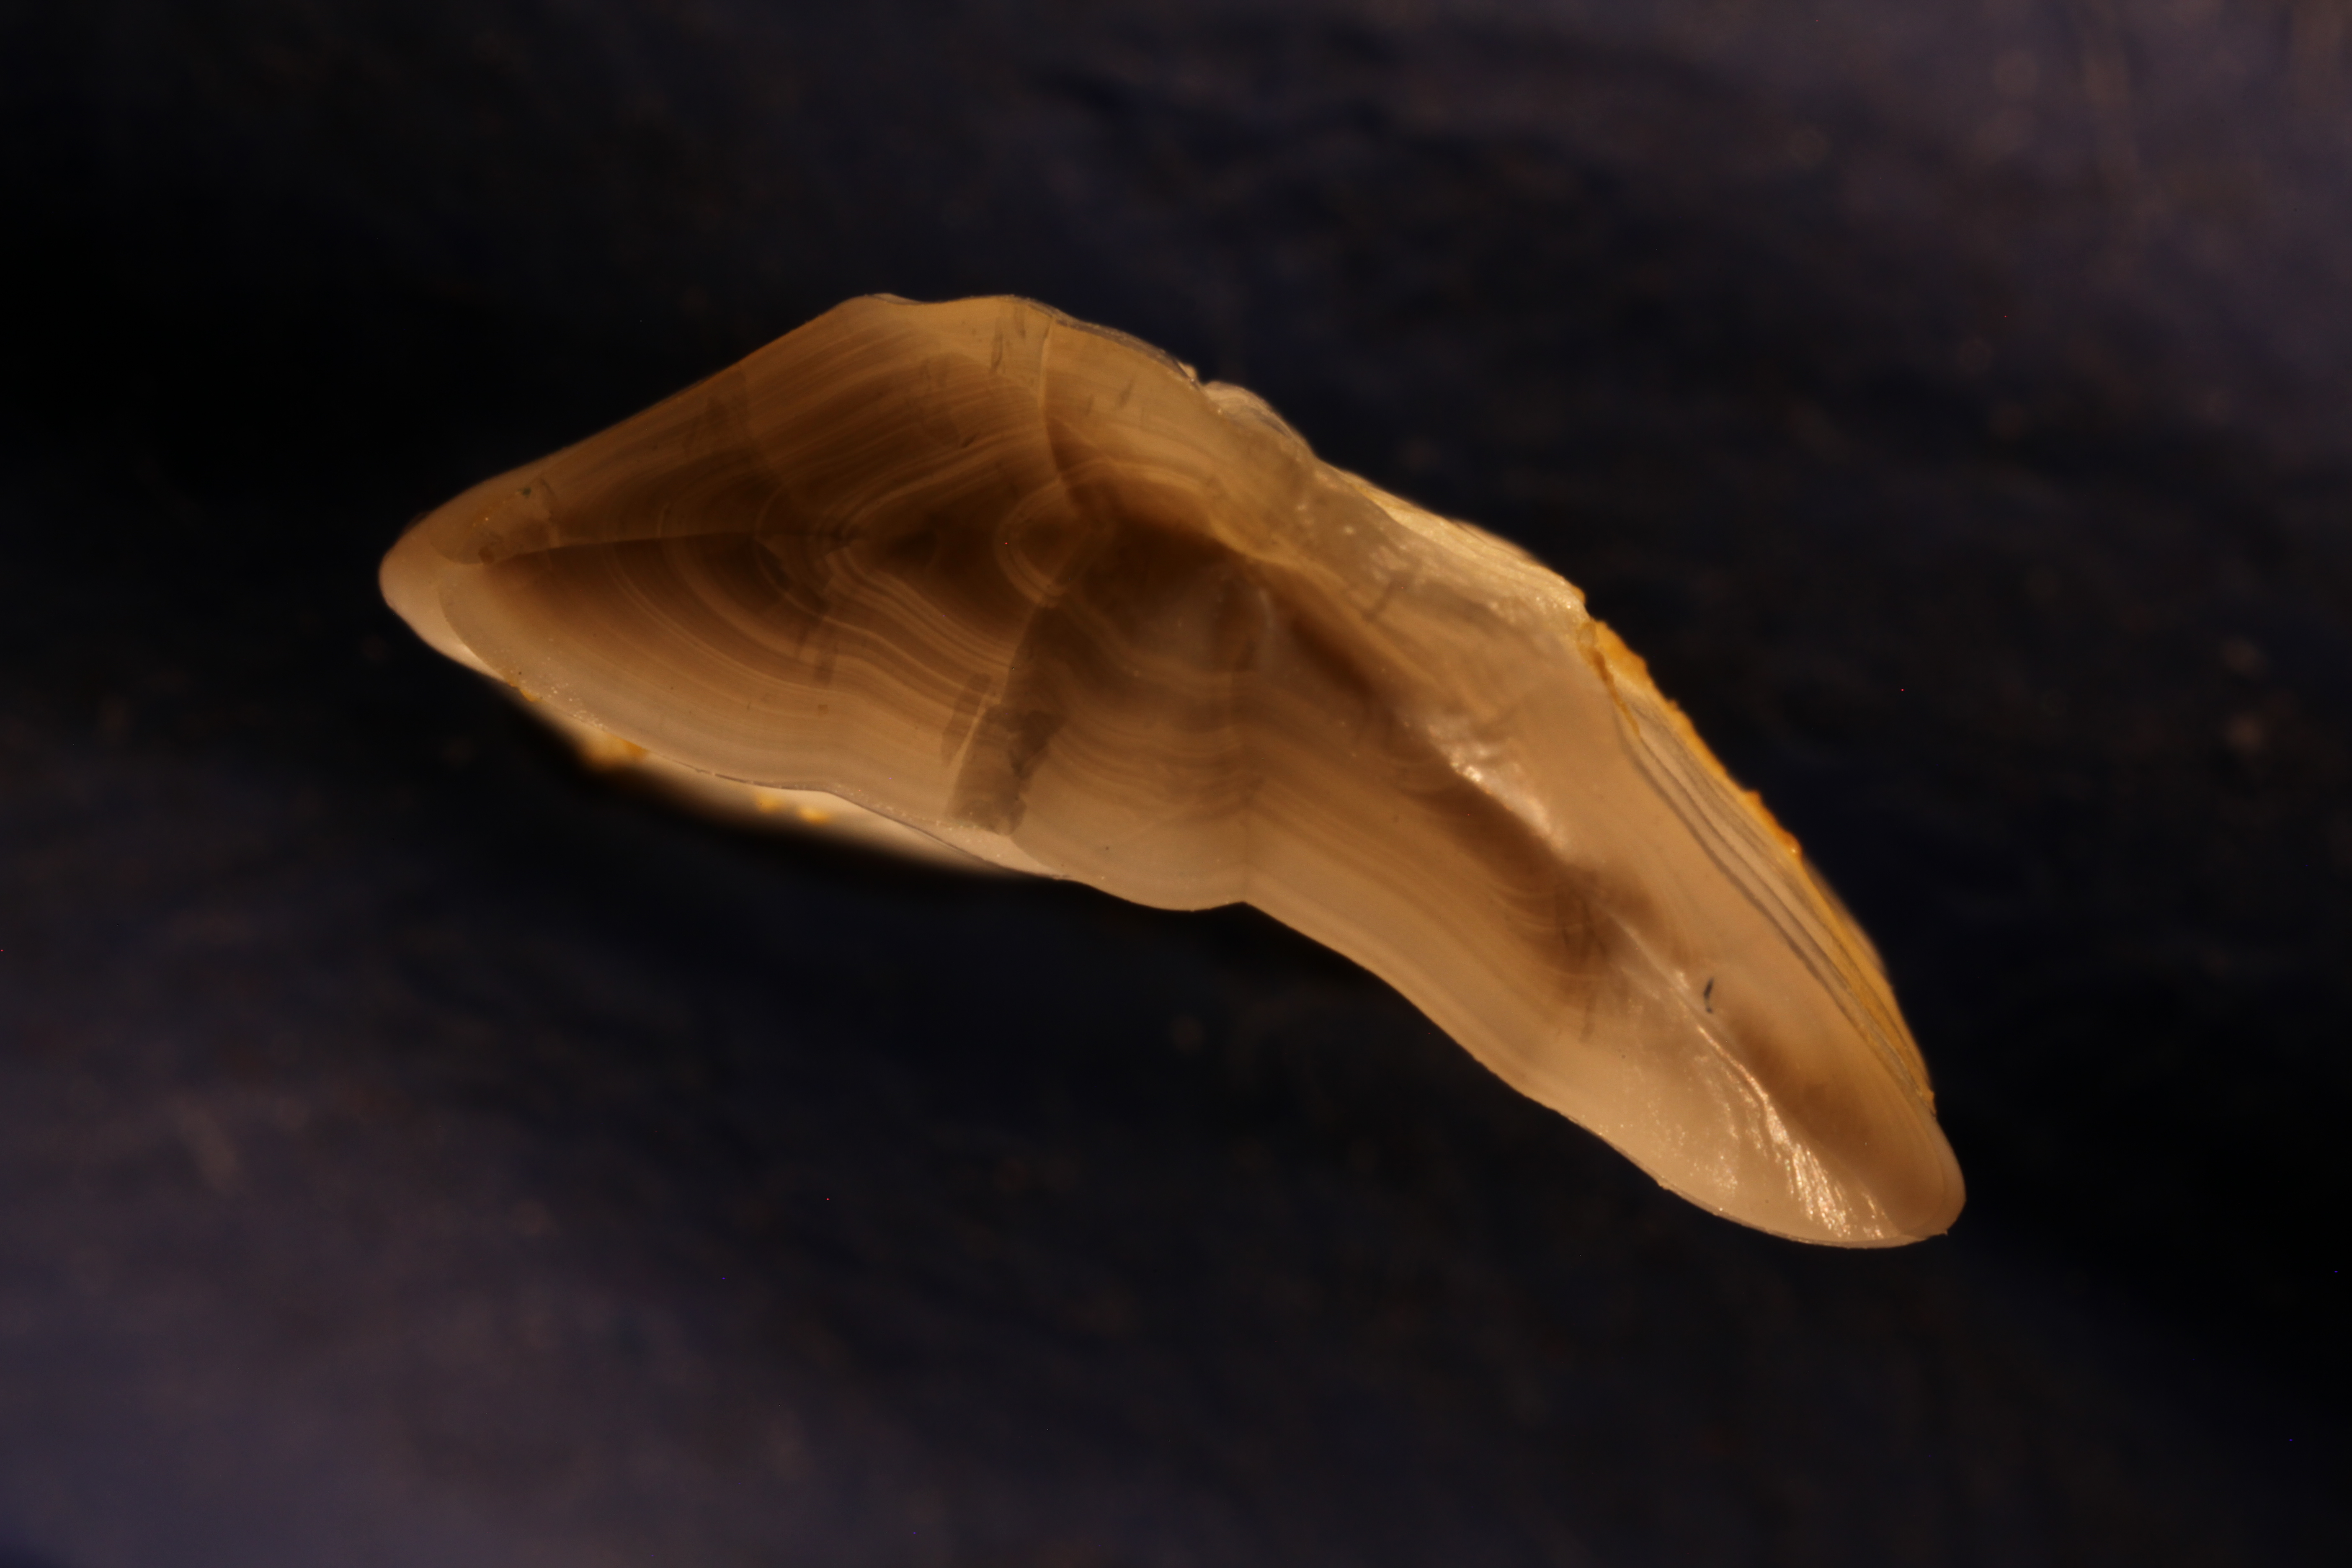
\includegraphics[scale=0.015]{otolith/IMG_0457_2016_70021.JPG}
  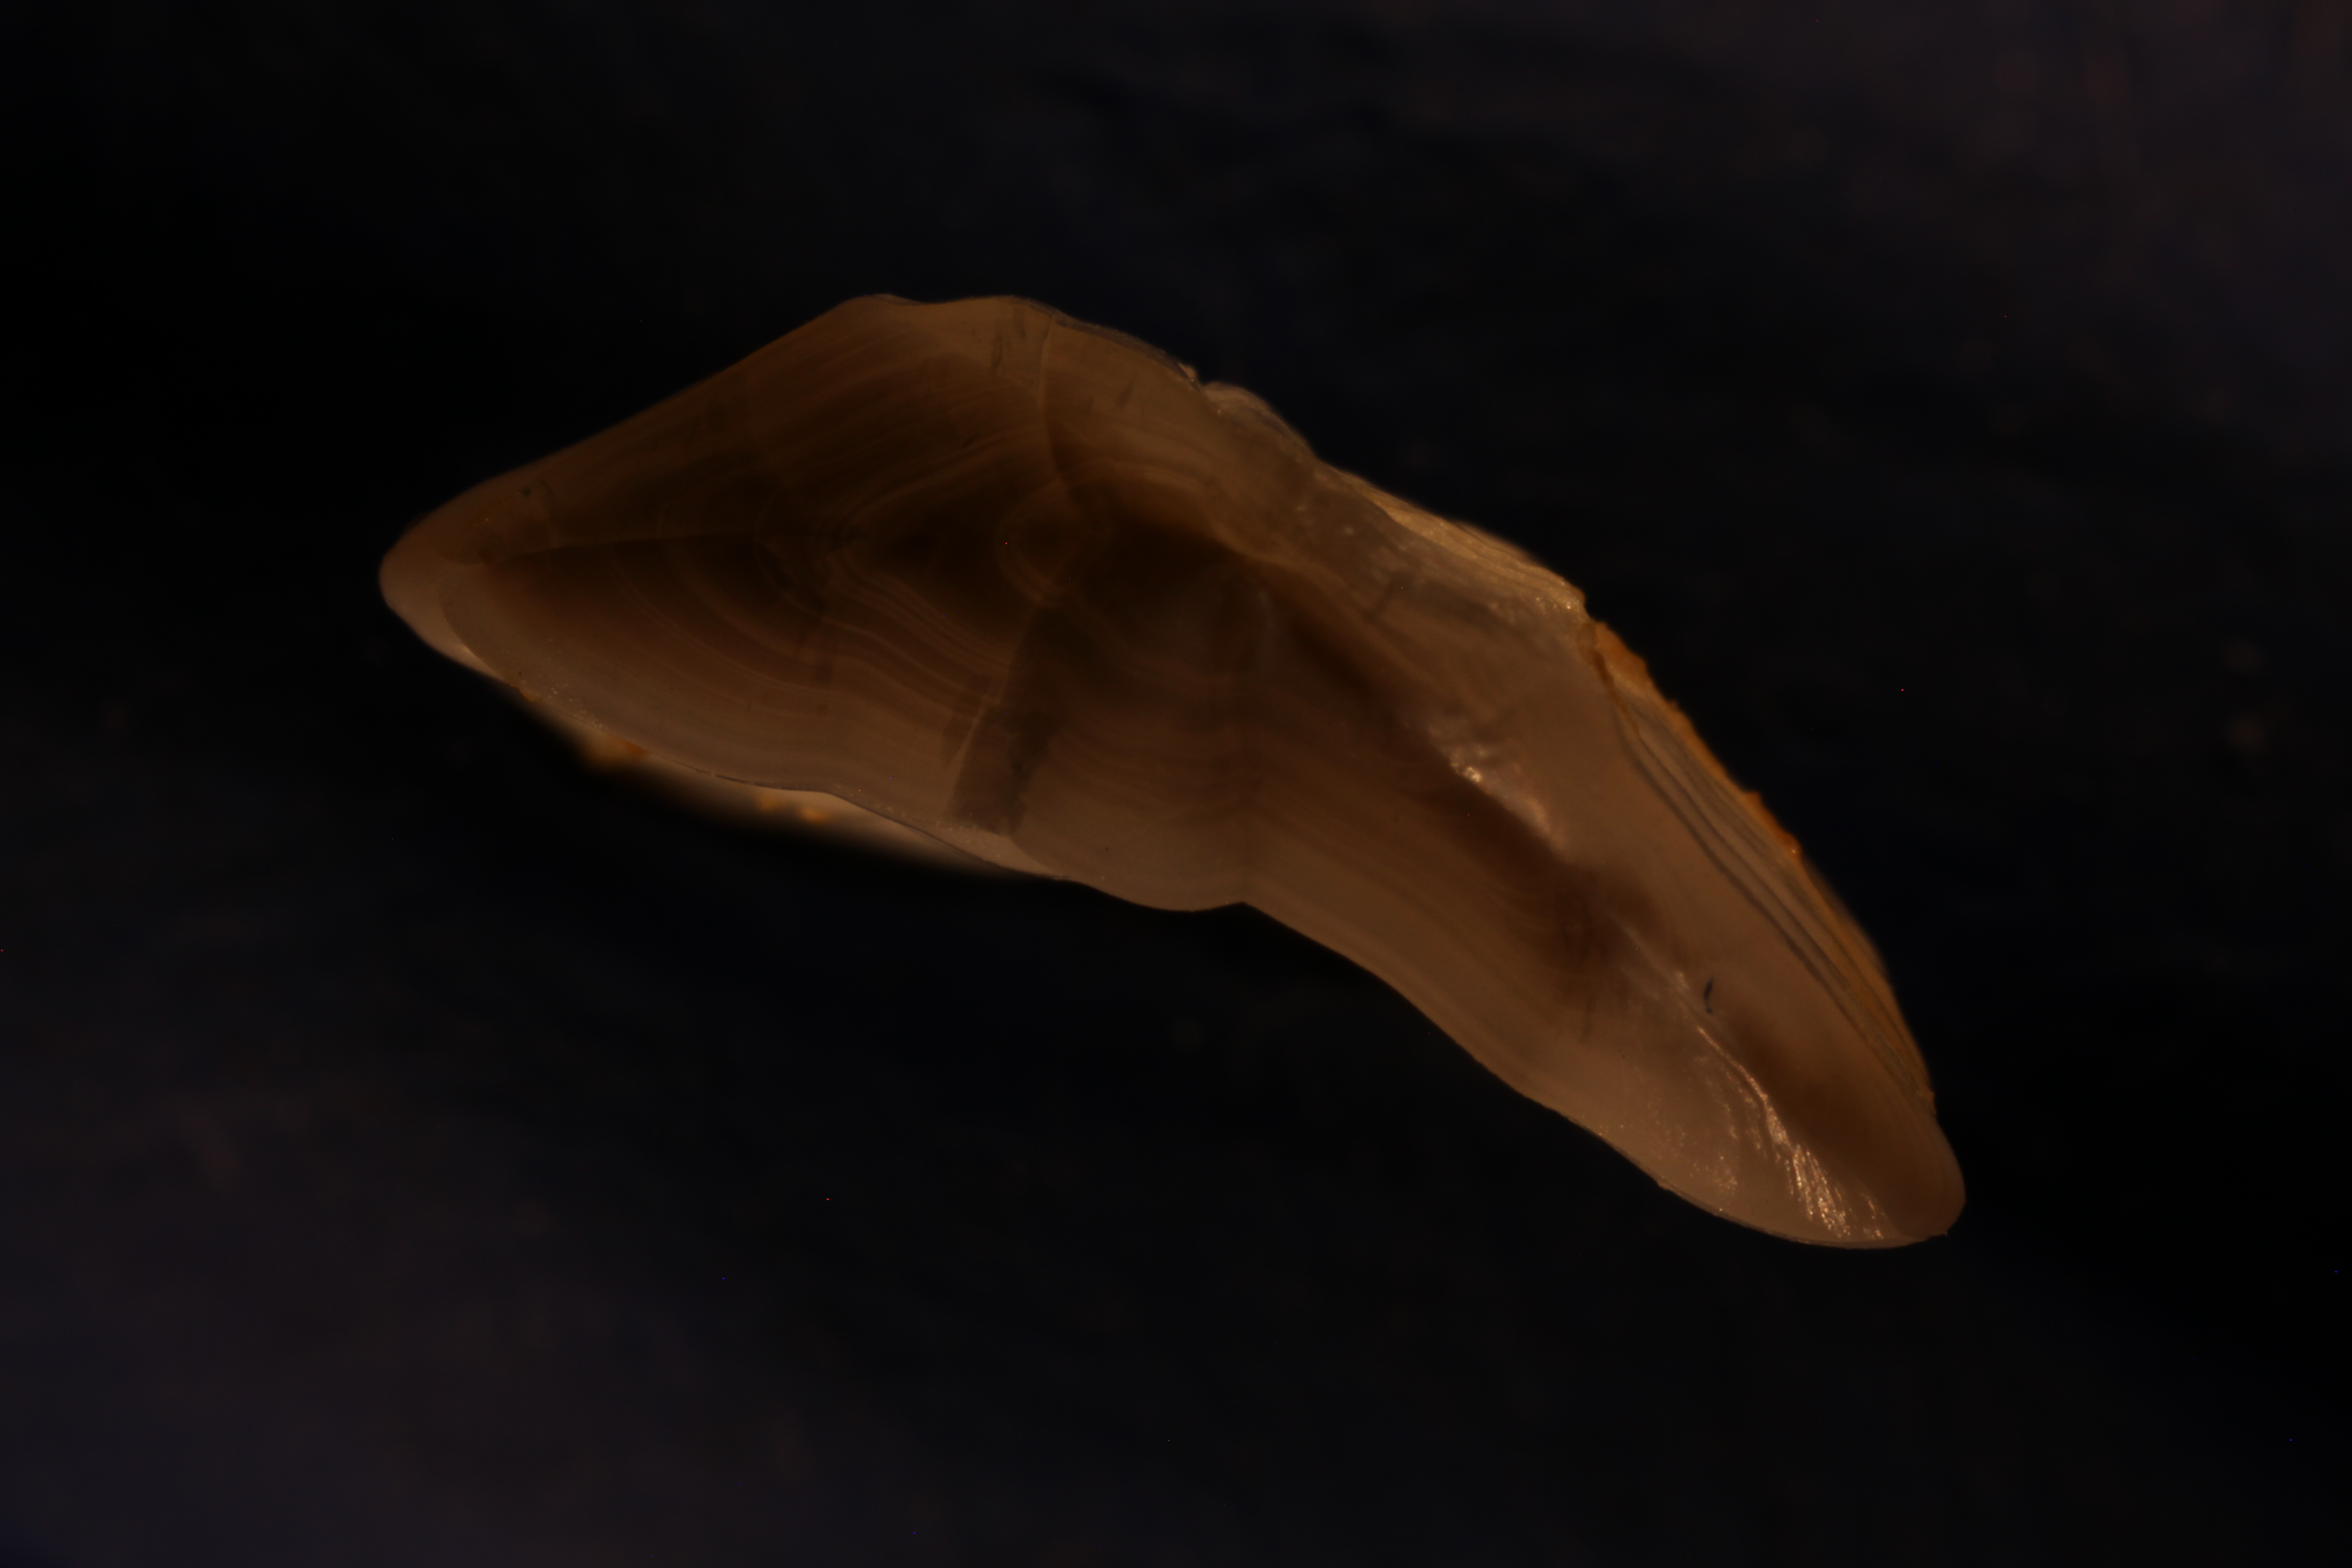
\includegraphics[scale=0.015]{otolith/IMG_0458_2016_70021.JPG}
  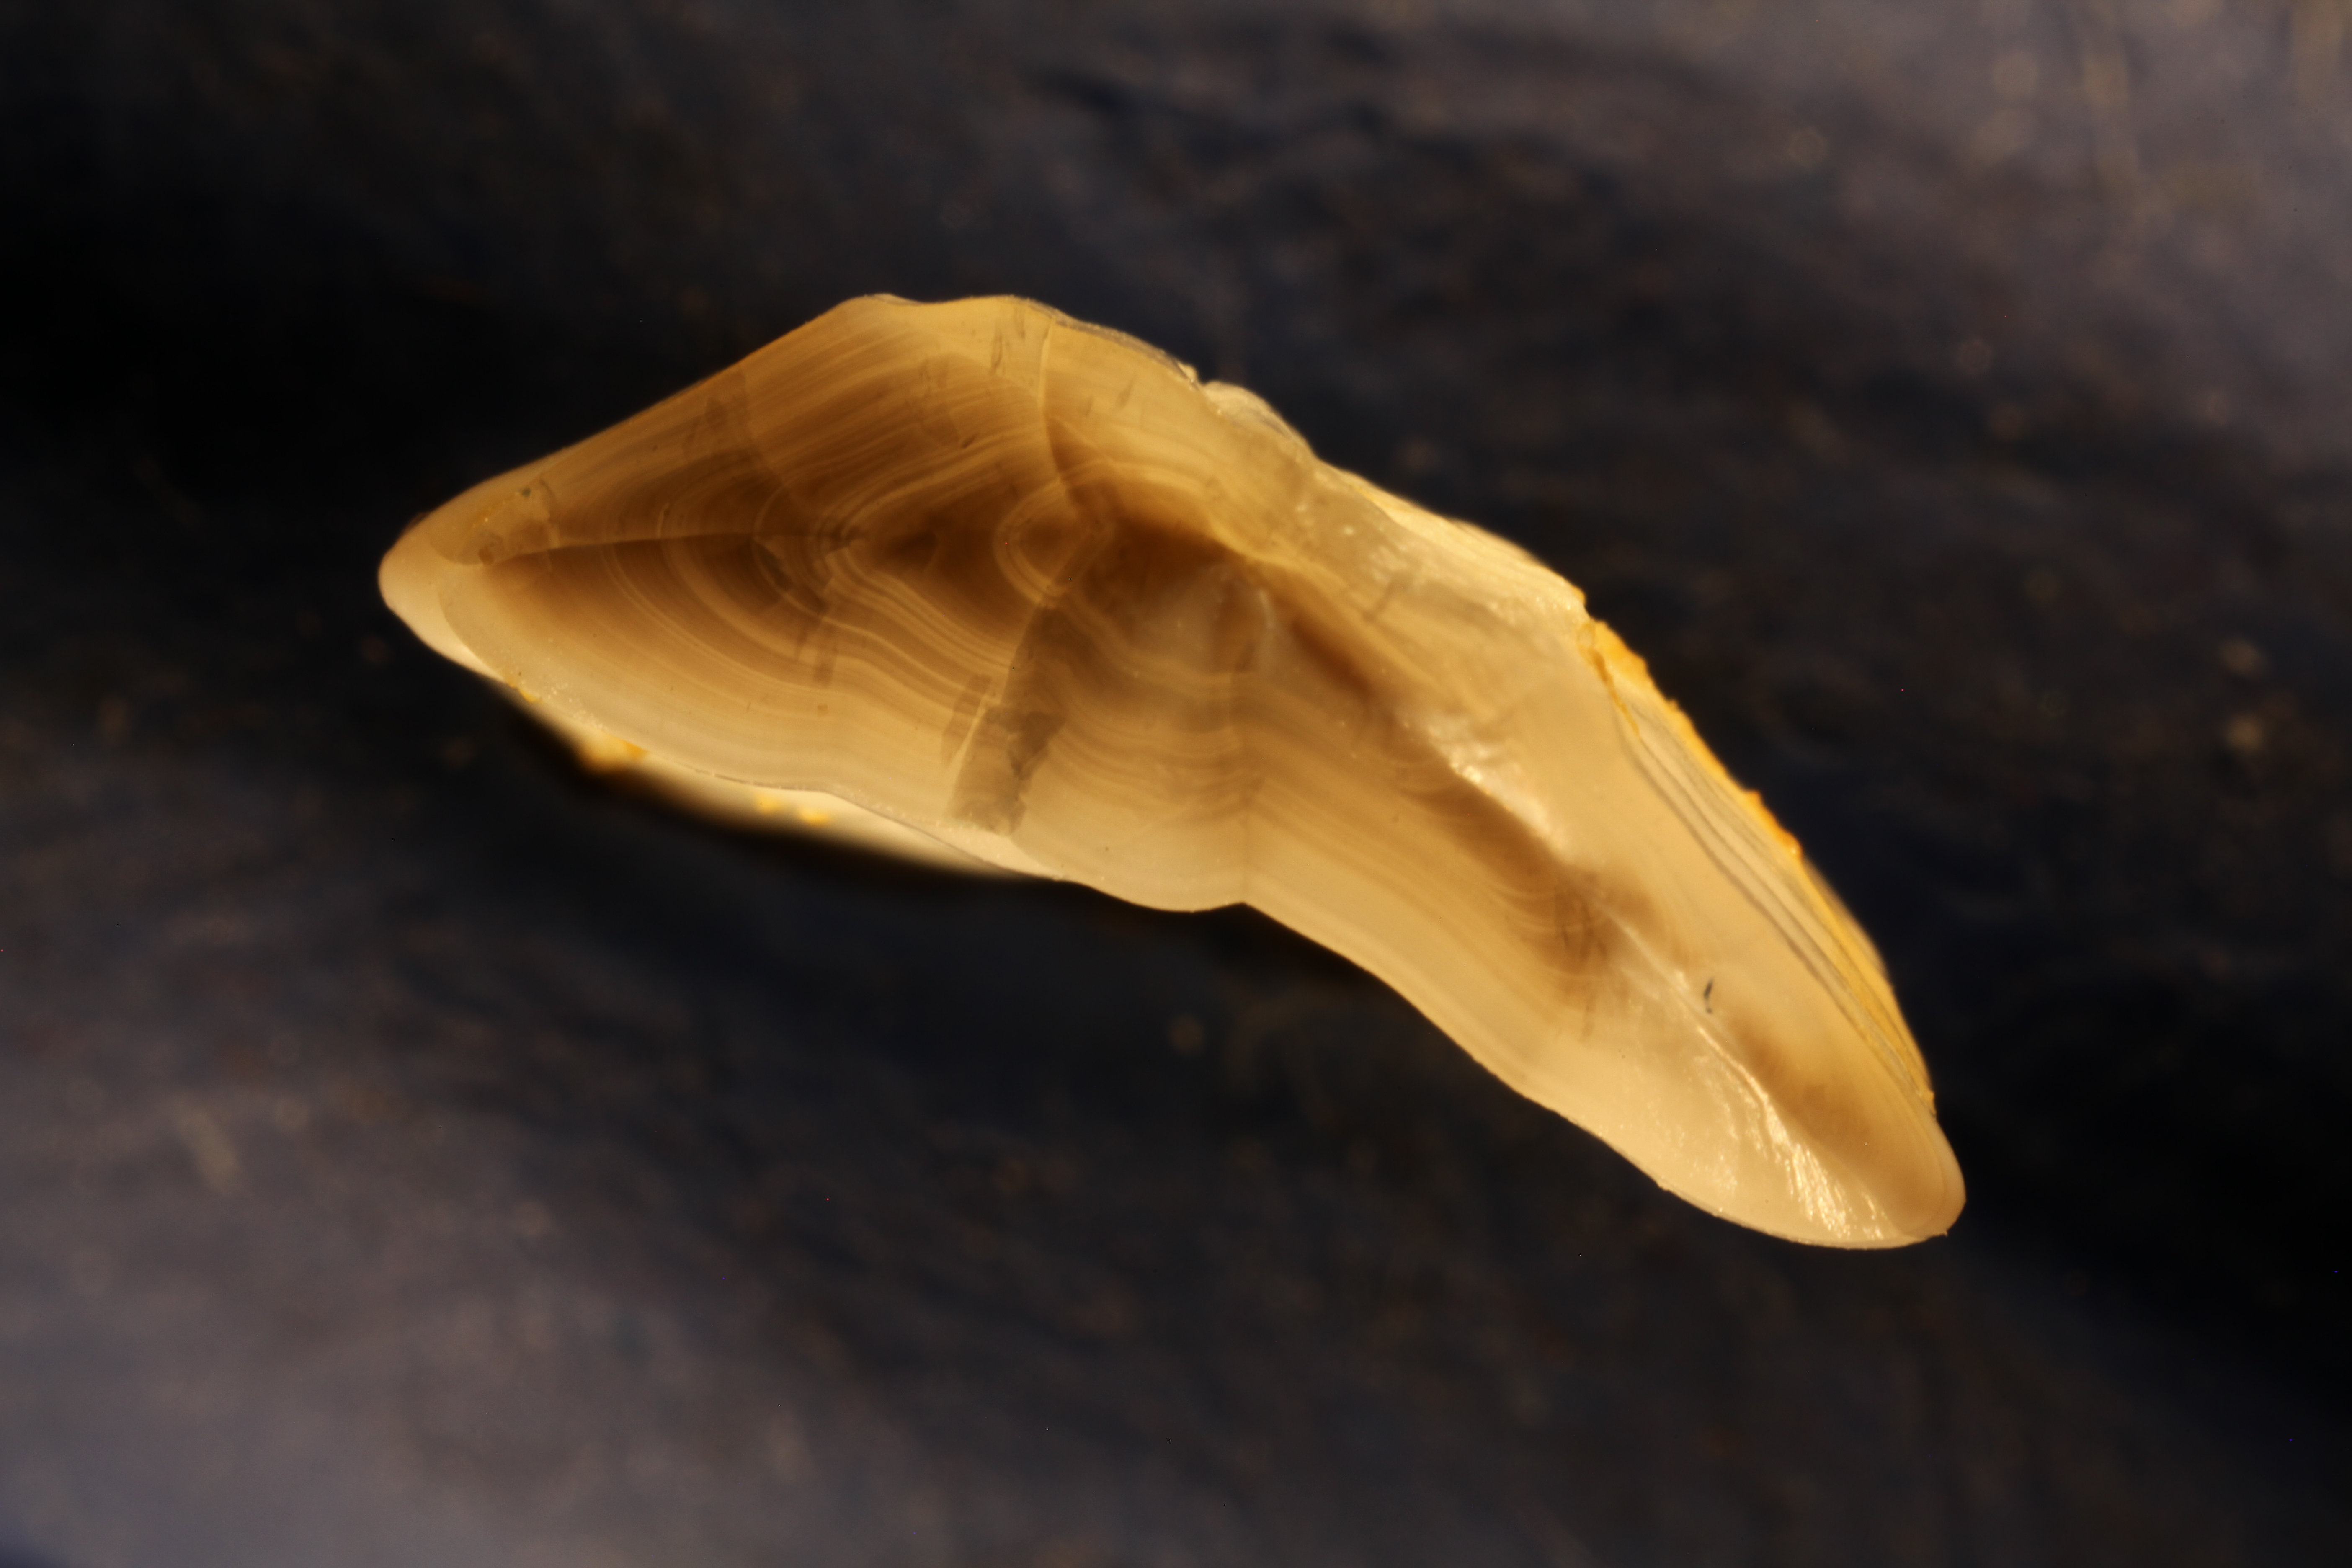
\includegraphics[scale=0.015]{otolith/IMG_0459_2016_70021.JPG} 

  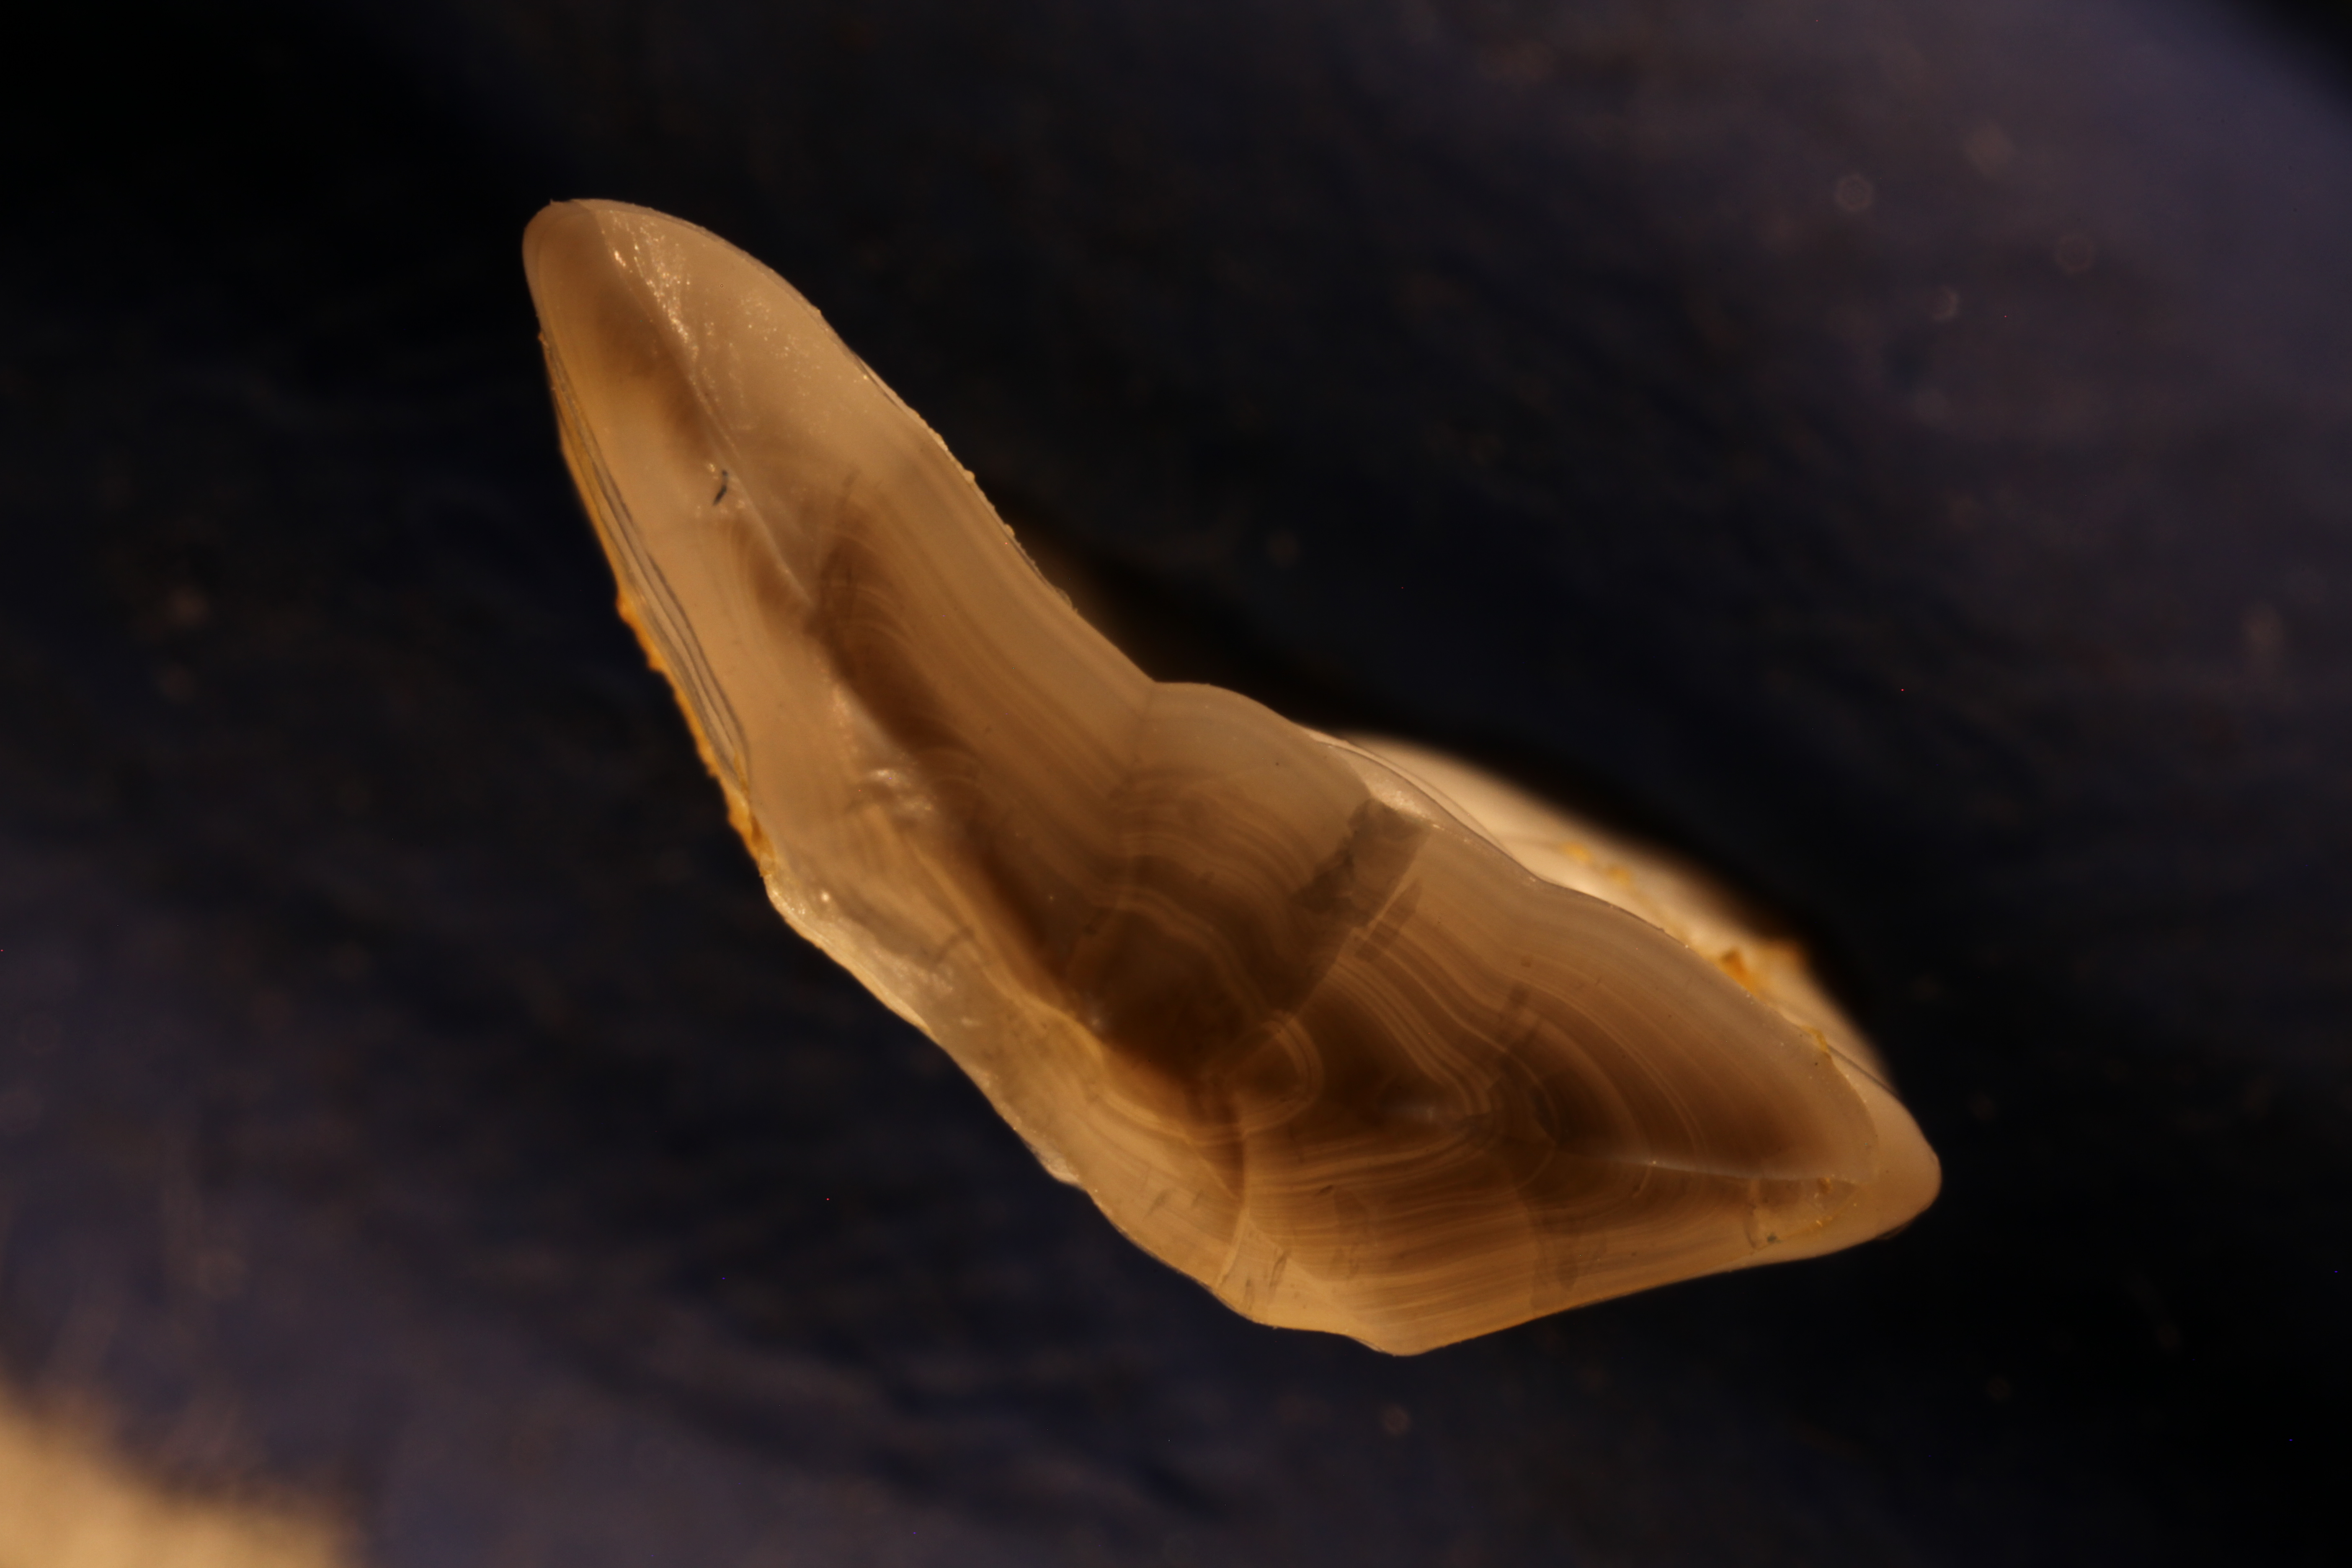
\includegraphics[scale=0.015]{otolith/IMG_0460_2016_70021.JPG}
  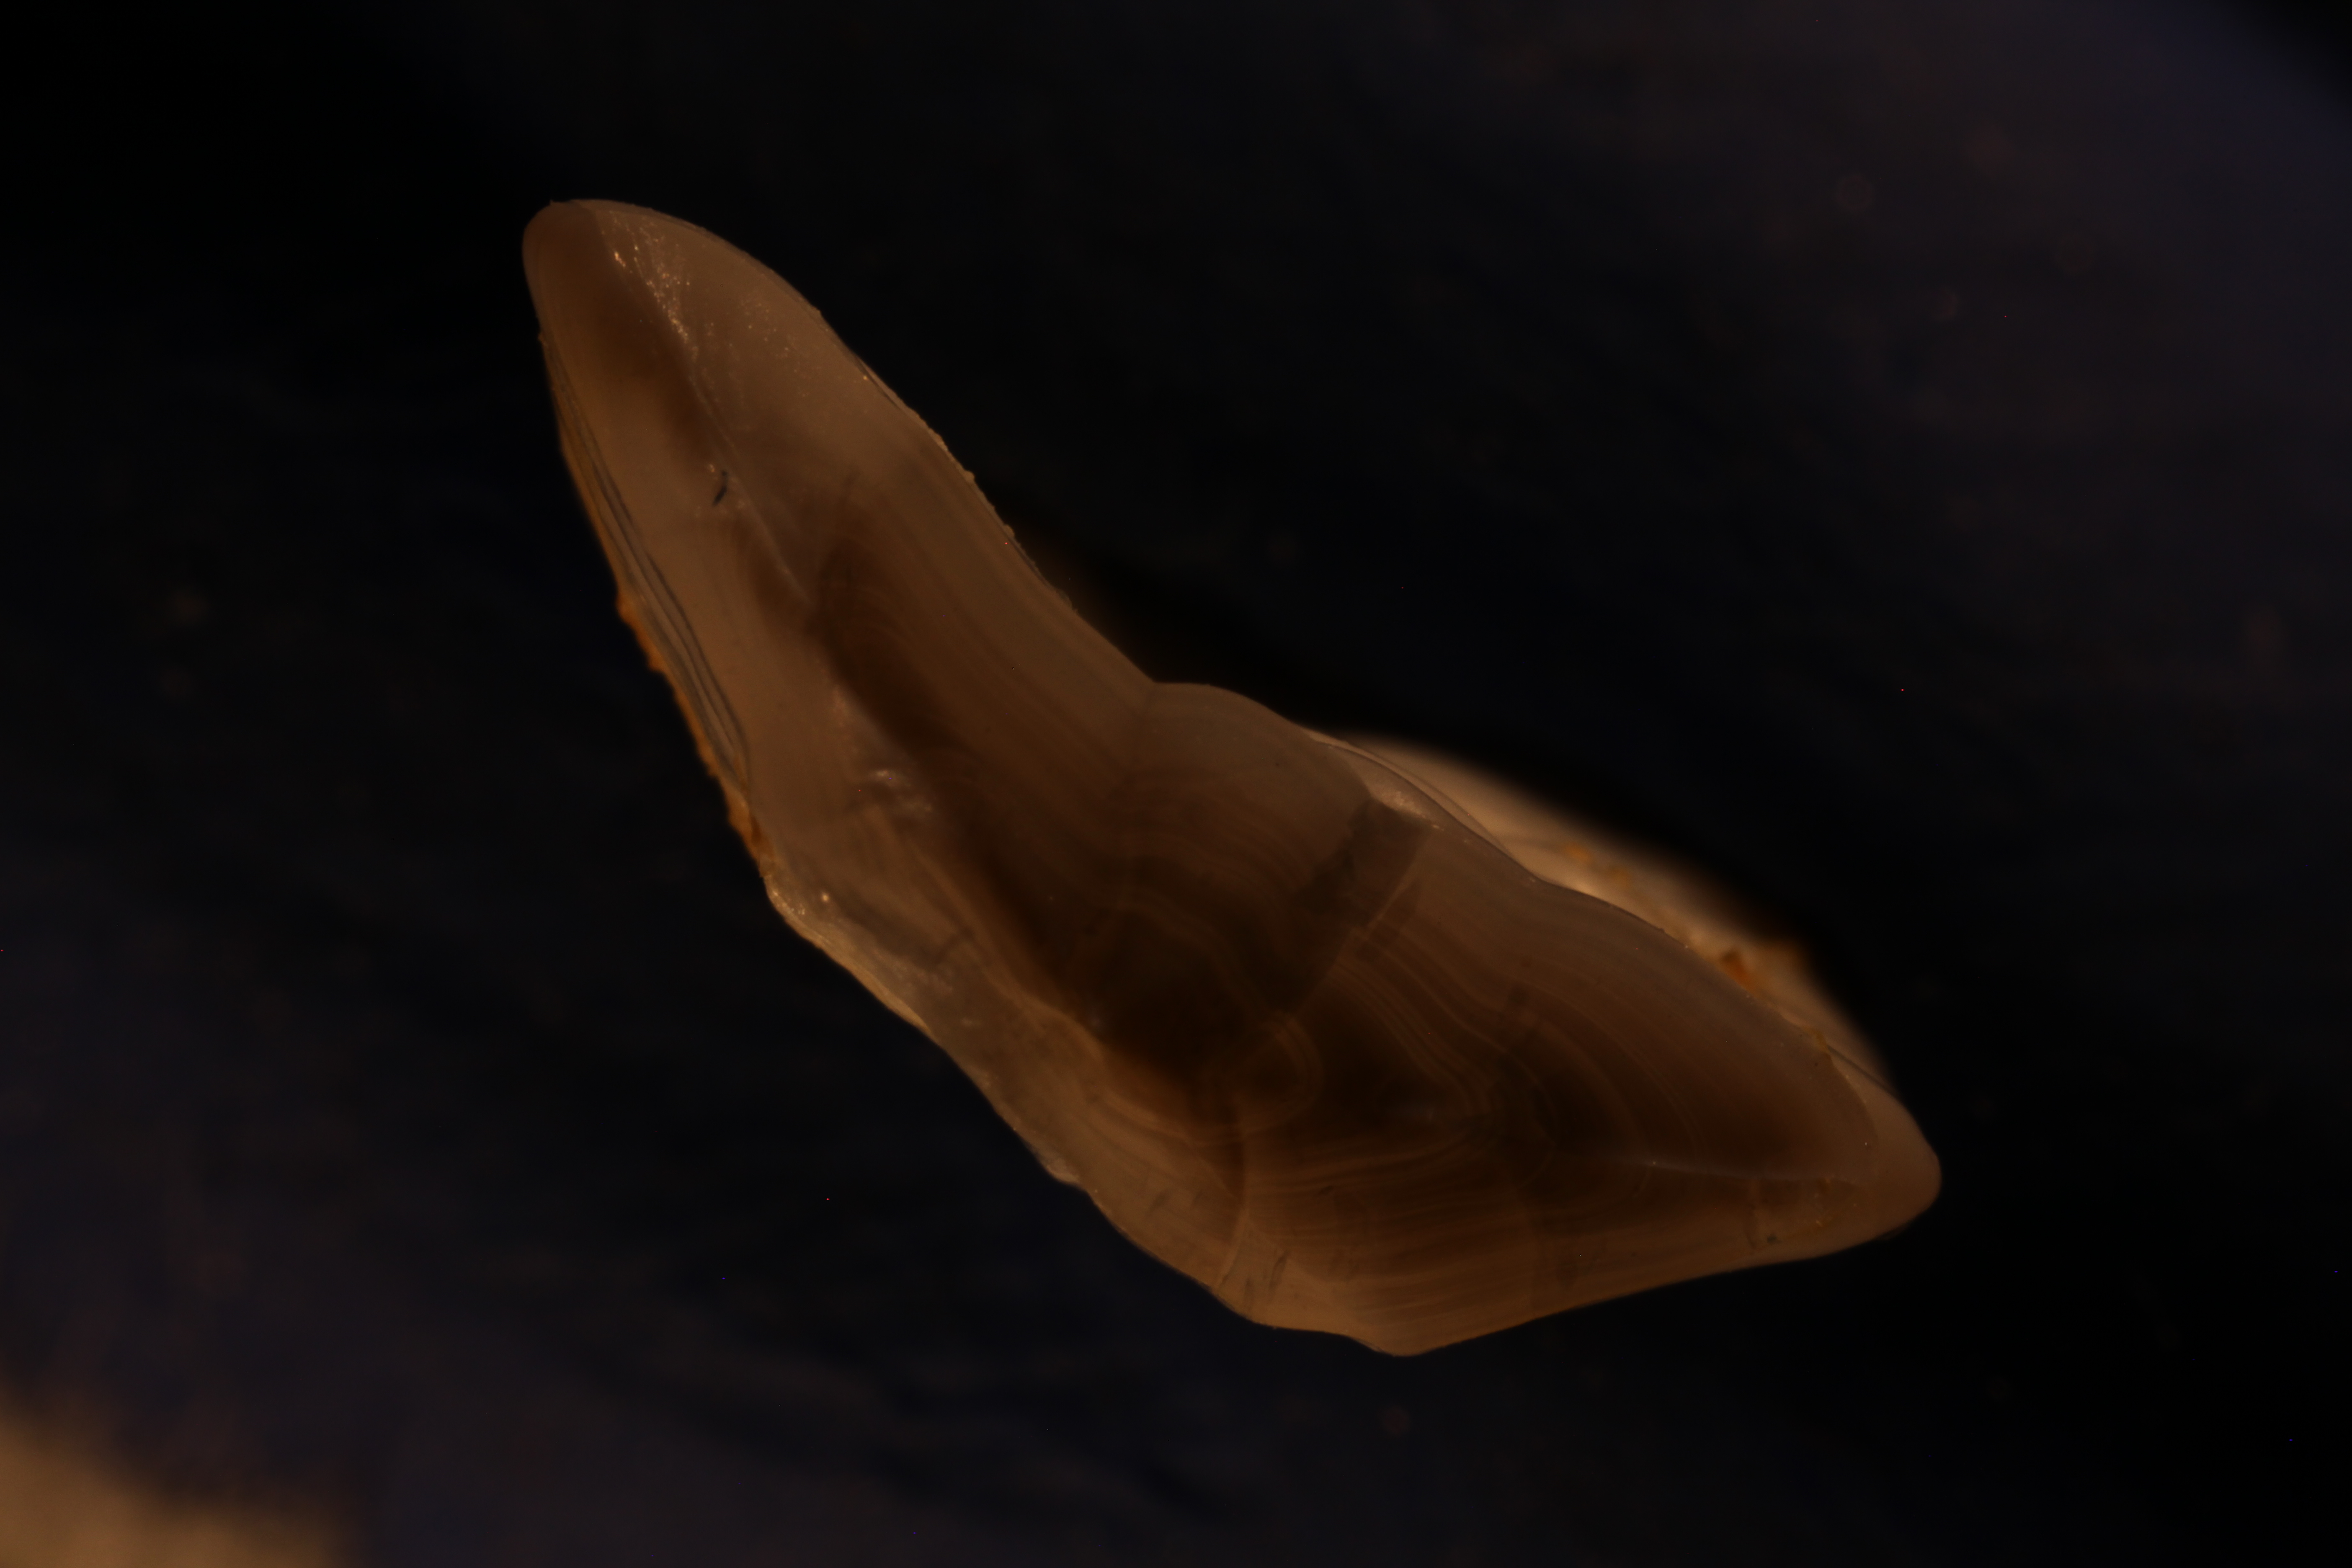
\includegraphics[scale=0.015]{otolith/IMG_0461_2016_70021.JPG}
  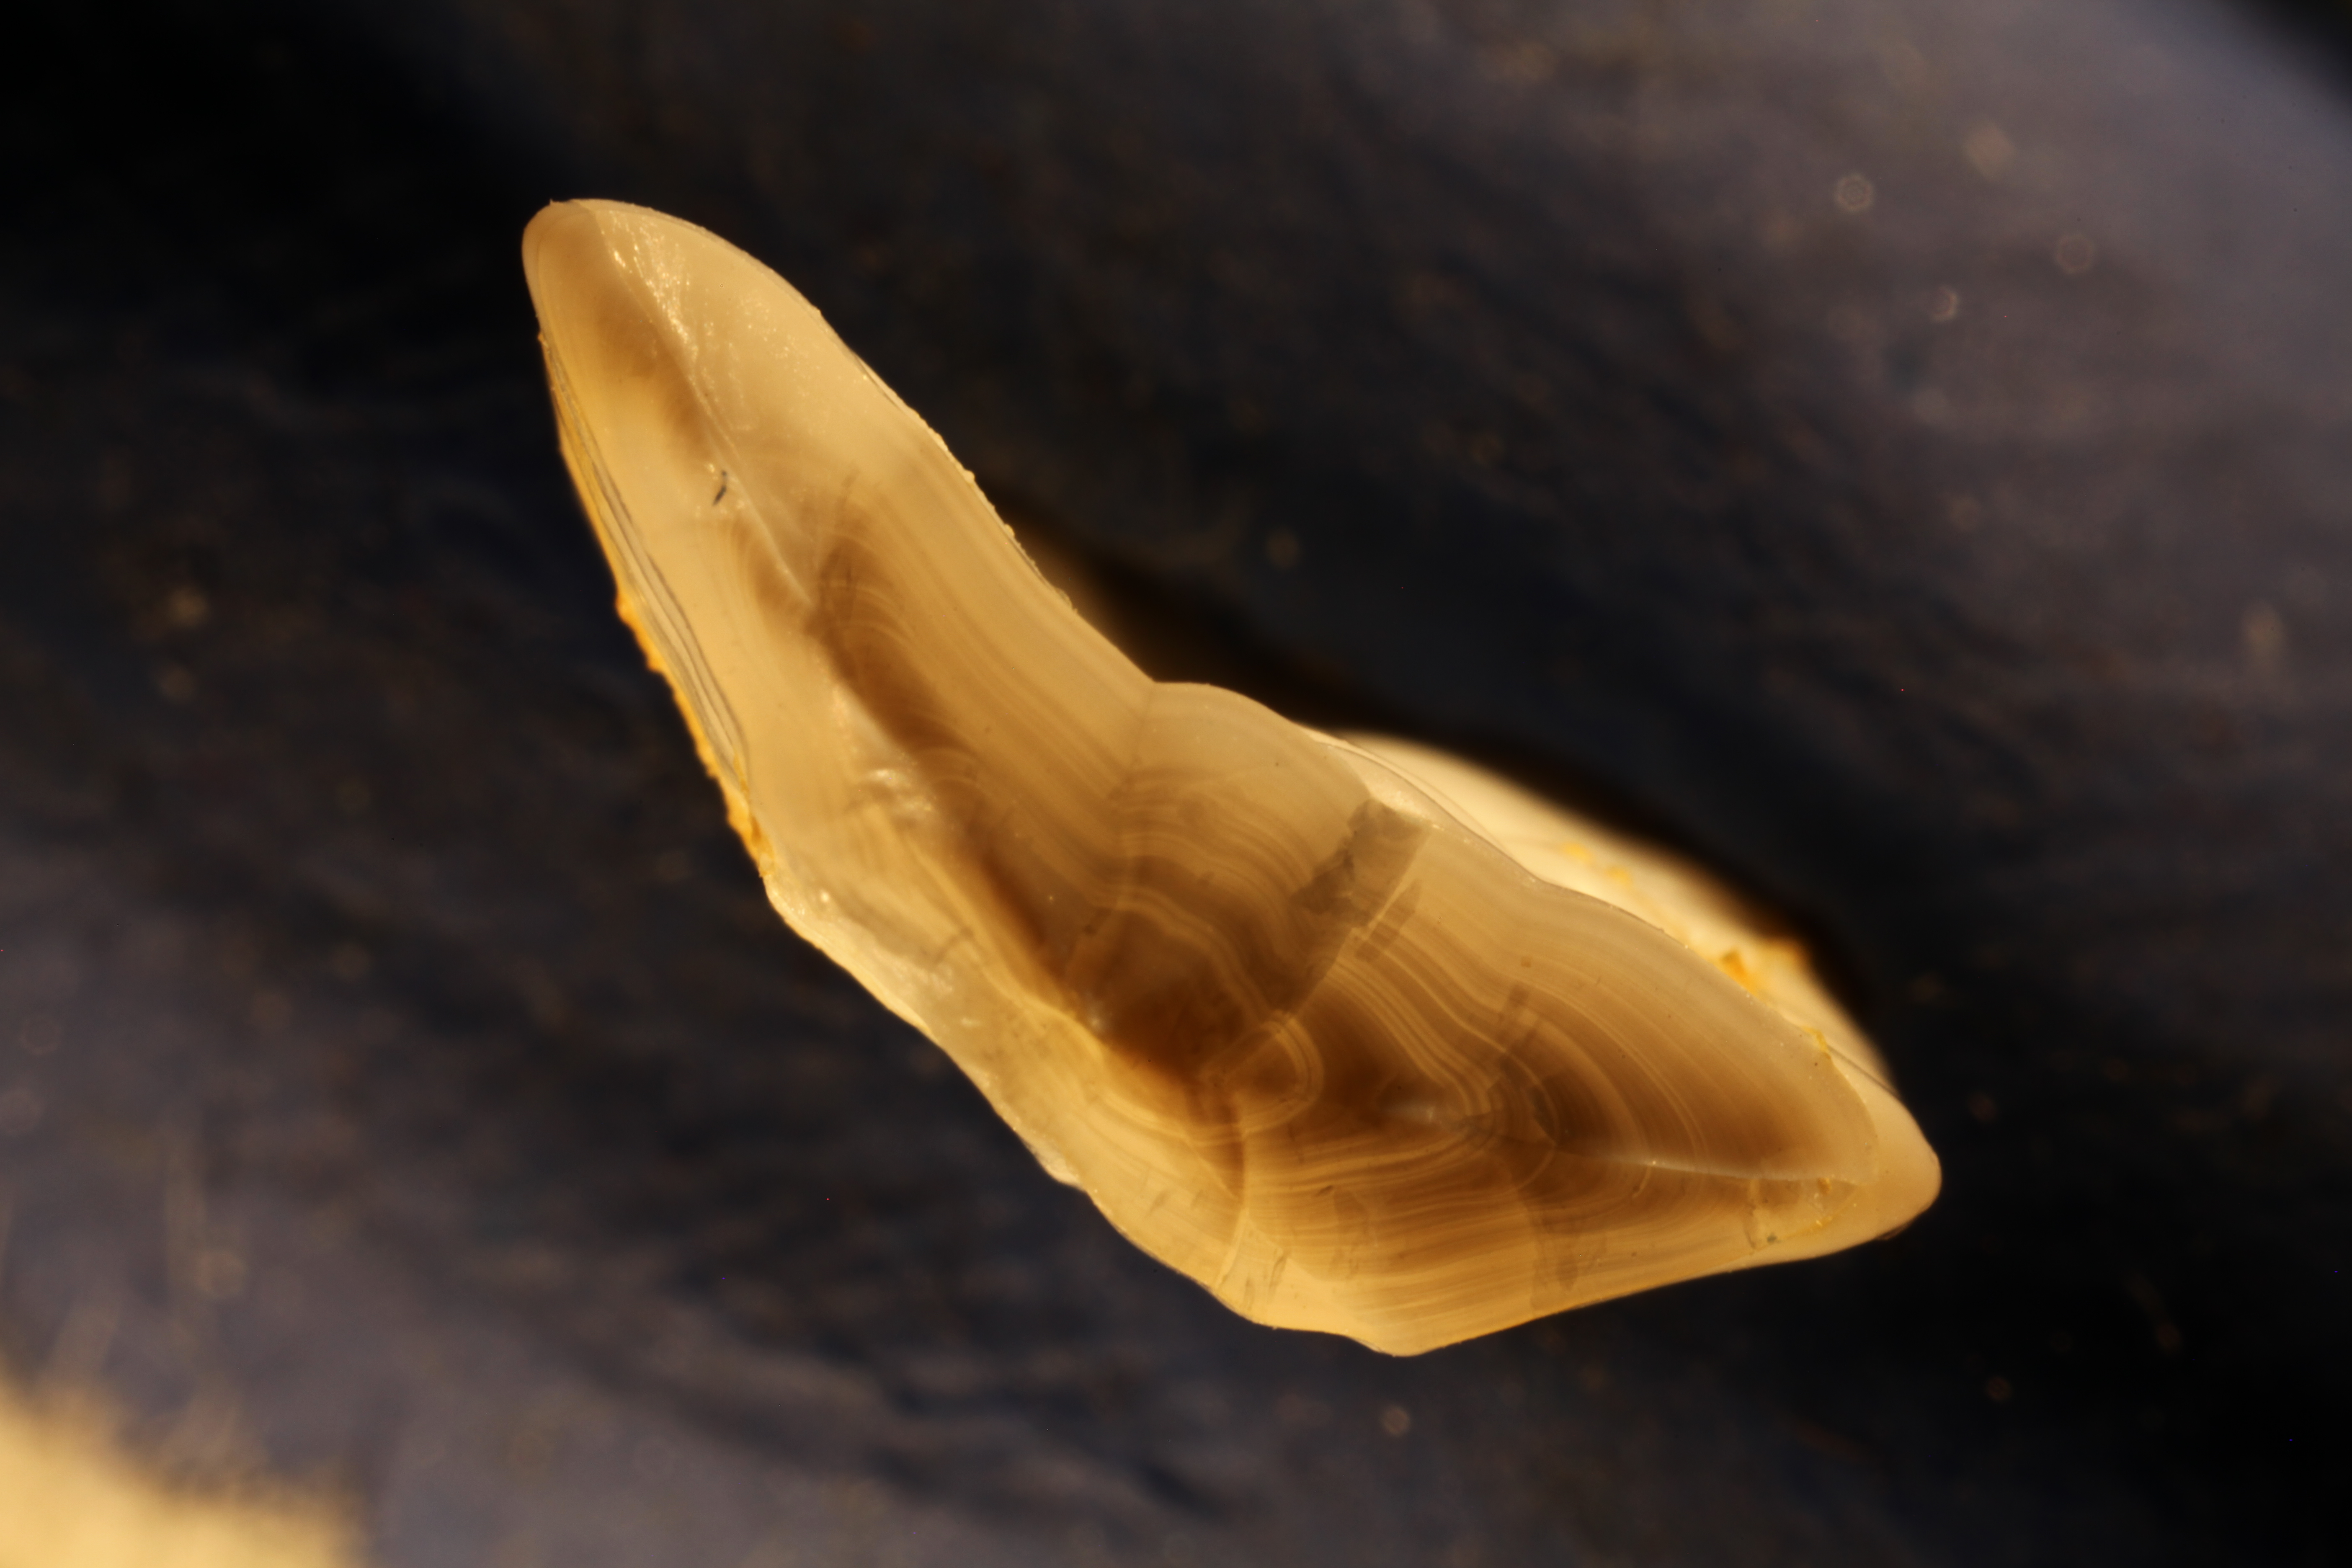
\includegraphics[scale=0.015]{otolith/IMG_0462_2016_70021.JPG}
  
  \label{marker1}
\end{figure}

The images were taken with a resolution of 3744$\times$5616 pixels.  The image light exposure varied depending on light condition outside, and was stored in the metadata of the JPG file. Typically the exposure order was middle-dark-light, then the rotation, and then middle-light-dark again,
but the order could vary. The exact order was  recovered by reading the 'ExposureTime' metadata property.

Figure \ref{marker2} shows the age distribution of the 5150 otoliths in the data set, and \ref{marker3} shows the age distribution selected at random from the data set used for
testing and consisting of 10\% of the whole data set or 515 otoliths.

\begin{figure}[h!]
  \centering
  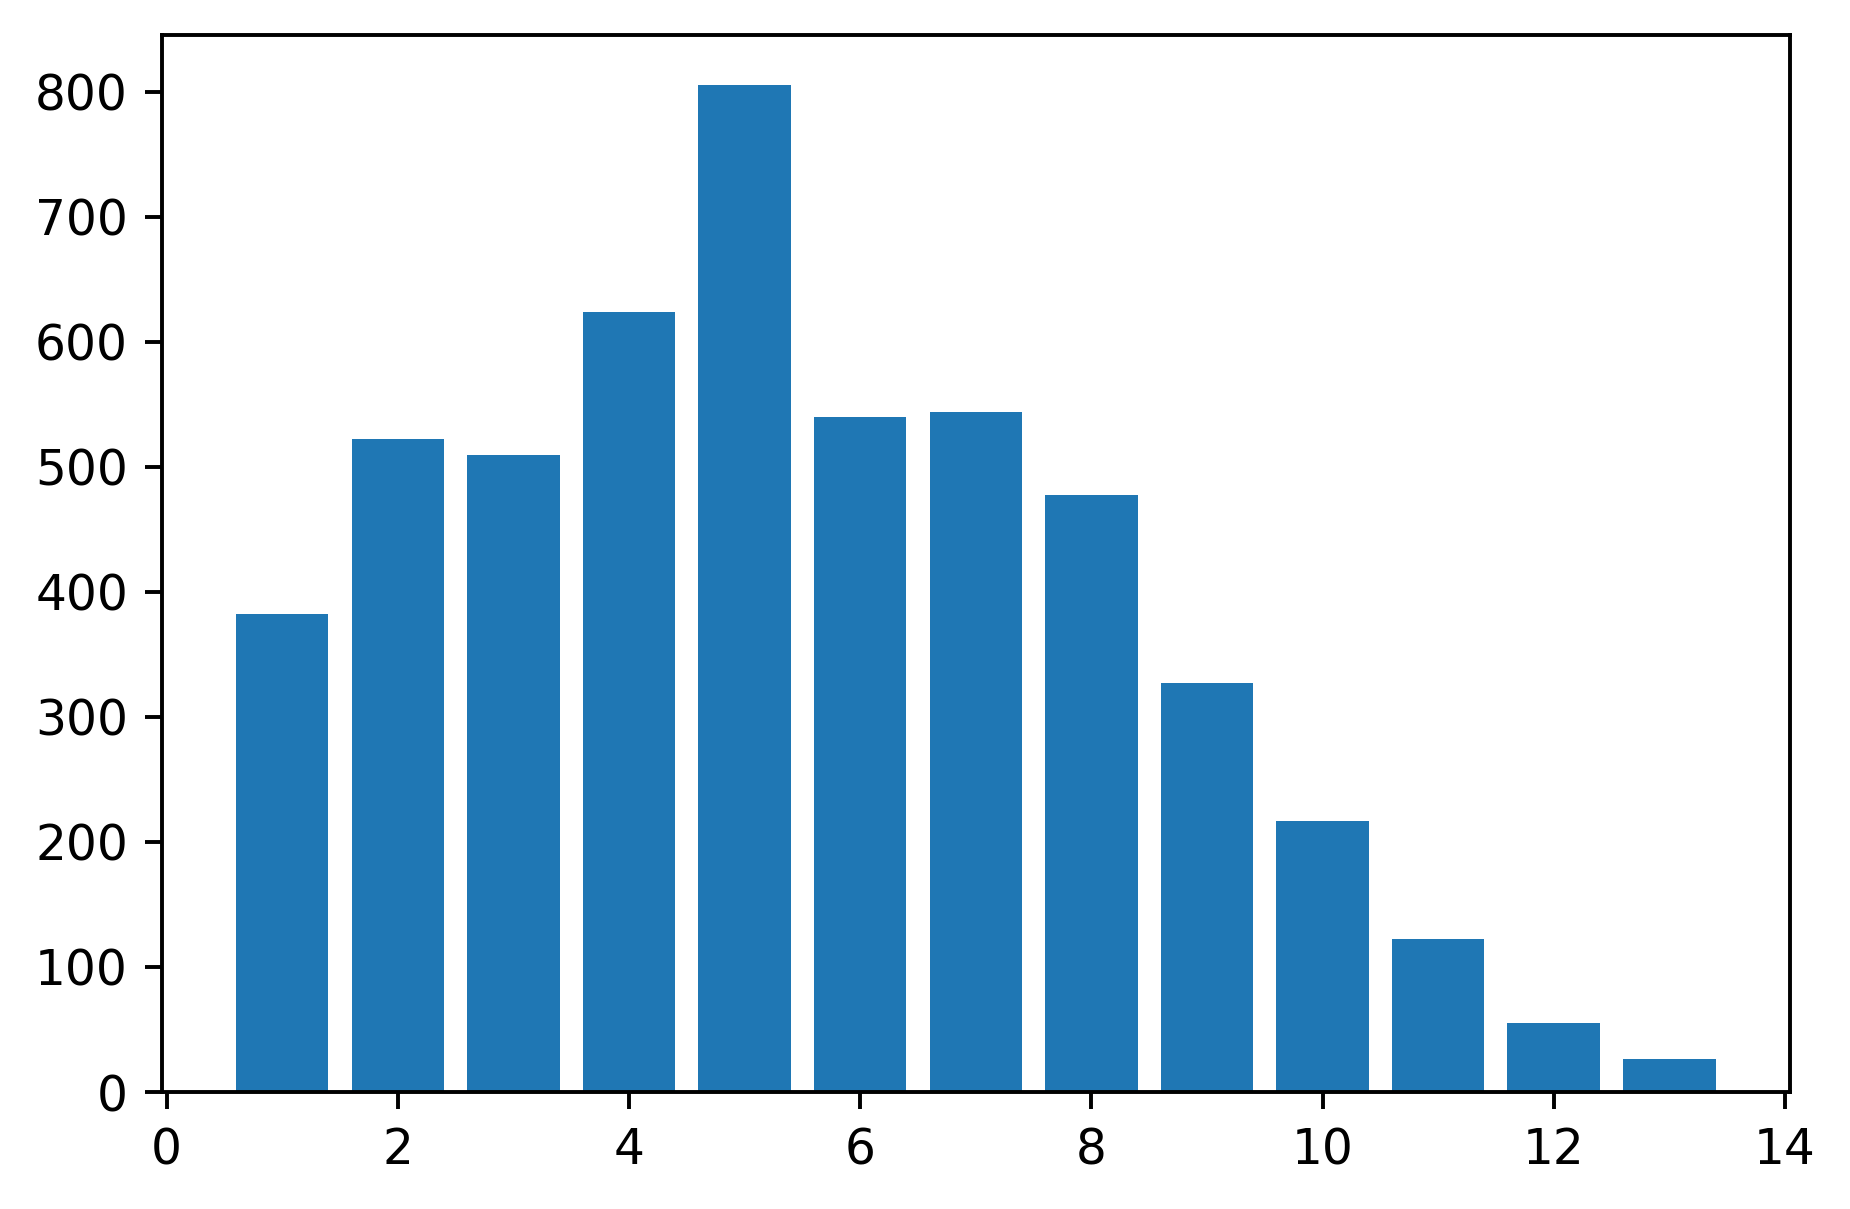
\includegraphics[scale=0.8]{distribution/age_distribution.png}
  \caption{Age distribution of all 5150 images}
    \label{marker2}
\end{figure}

\begin{figure}[h!]
  \centering
  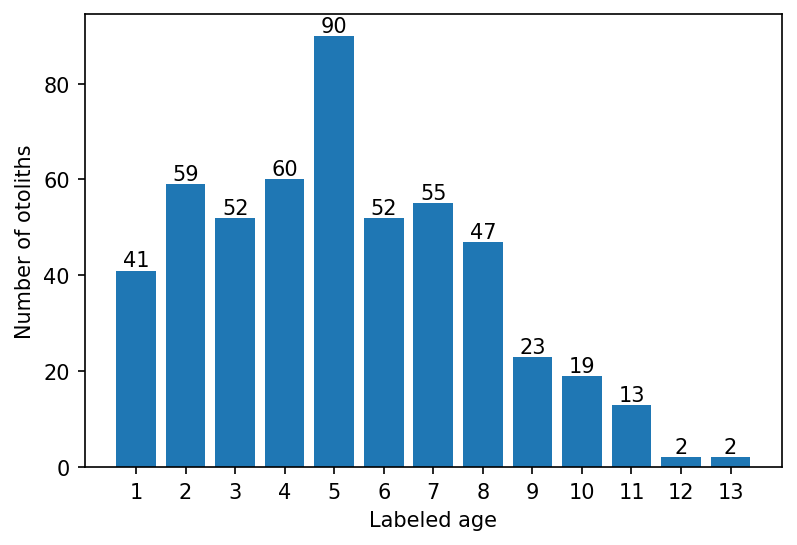
\includegraphics[scale=0.80]{distribution/age_distribution_test.png}
  \caption{Age distribution of 515 images from the test set}
  \label{marker3}
\end{figure}

\subsection*{Convolutional neural network architecture}

\begin{table}[hbt!]
\caption{EfficientNet and EfficientNetV2 models trained with image exposure.
The models are numbered for reference of chapter on ensembles later}
\begin{tabular}{ |l|c|c|c|c|c|c| }
\hline
CNN family / & \multicolumn{3}{c|}{EfficientNet} & \multicolumn{2}{c|}{EfficientNetV2} \\
Image exposure & B4 & B5 & B6 &Medium &Large  \\ 
\hline
Minimum & 1 & 2 & 3 & 4 & 5  \\ 
Medium & 6 & 7 & 8 & 9 & 10  \\ 
Maximum & 11 & 12 & 13 & 14 & 15  \\ 
All (3 images) & - & - & - & 16 & 17  \\ 
\hline
\end{tabular}
\label{table1}
\end{table}
Each CNN was trained using transfer learning by loading ImageNet weights. The images were resized from 3744$\times$5616 pixels to between 380$\times$380 and 528$\times$528 pixels
depending on the architecture. The pixel values have a range between 0 and 255, which was normalized to between 0 and 1. While test set size prediction was done on 380$\times$380 and 384$\times$384 pixels. To investigate the image-taking protocol described in \citep{codOtolithsMyers} we also trained on 9-channel images by stacking 3 RGB images representing 3 different lighting exposures. Using Timm\citep{rw2019timm}, the imageNet weights were duplicated on the input layer to accommodate 9 channels. The three images used were of dark, medium and light exposure of the first orientation. Figure \ref{marker4} shows an example of the 4 exposures used for training and testing the models. 

\begin{figure}[h!]
  \caption{Otolith from 2013, read age: 6 years, and with light exposure: medium, low, high, 
  and expectation per channel of the three exposures (9-channels). }
  \centering
  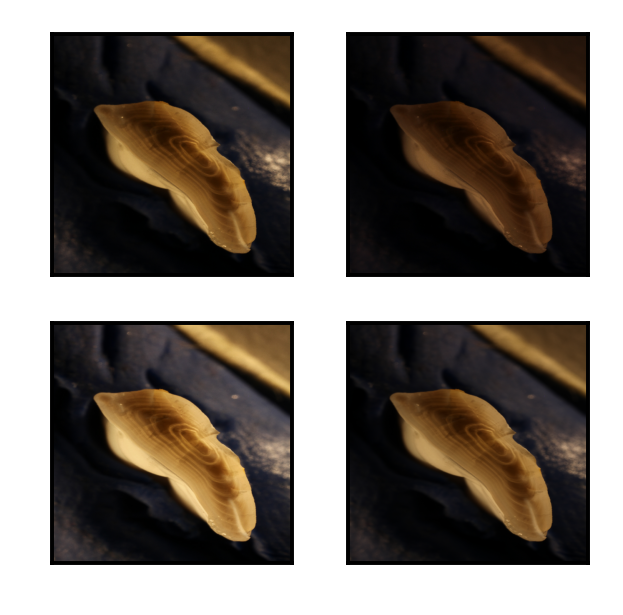
\includegraphics[scale=1.0]{otolith/2013_70174_Nr06_age09_IMG_0031_32_33.png}
  
  \label{marker4}
\end{figure}

CNNs were selected based on performance on the ImageNet benchmark and availability of open-source implementations with imageNet weights. The imageNet benchmark is for classification while we treated aging as a regression problem \citep{moenetal} \citep{vaboeetal}. The last layer of the CNNs was modified to output a linear output. In the EfficientNetV2 family we did this by applying three multi-layer perceptron layers going from 1280 output of the last hidden layer to a dense 256-layer, 
then a leakyRelu \citep{DBLP:journals/corr/XuWCL15} layer, then a dense 32-layer, then a leakyRelu layer, and finally a linear output layer. For EfficientNet we only changed the last layer from softmax output to a linear output.

To each fold we normalized the age on the training-set by subtract the mean and scaling to unit variance. The normalization was then applied to the validation and test set. Test set predictions were obtained by applying the inverse transform.

\subsection*{Implementation and training}

EfficientNetV1 B4, B5, and B6 were imported and modified with TensorFlow \citep{abadi2016tensorflow} and Keras \citep{keras} software packages in Python. Computation was done using CUDA 11.1 and CuDNN with Nvidia(Nvidia Corp., Santa Clara, California) A6000 accelerator card with 48 GB of GPU memory and P100 cards with 12 GB of GPU memory,
EfficientNetV2 Medium, and Large were imported and modified with the PyTorch \citep{NEURIPS2019_9015}  and Timm \citep{rw2019timm} software packages. Computation was done on P100 and RTX 3090 with 24 GB of GPU memory. Pretrained weights for EfficientNet were available from Keras, and pretrained weights for EfficeintNetV2 were available from Timm.

Augmentation was applied to the training-set. The images were augmented using rotation between 0 and 360 degrees, and reflection by the vertical axis. 

The cost-function used was mean squared error (MSE)
while the metric used for evaluating the models and comparing it to expert readers was accuracy. Accuracy was obtained by rounding the floating point number predictions to nearest integer and comparing the age classification against the true labels.

% k-fold cross validation
The dataset of 5150 otoliths were divided into a training set constituting 90\% of the otolith images (4635 otoliths) and a test set of 10\% (515 otoliths).
To get the most out of a small data-set we applied 10-fold cross-validation on the training set. This meant that 10\% of the training set were used for validation and 90\% (81\% of the whole data set) were used for the actual training for each fold. Consequently 10 different models were trained with a different set of 463 images used for validation in each fold, i.e. each data point participates in the validation set once and in the training set 9 times. Among the 10 fold models the one with the best MSE was chosen. The best model-parameters on the validation set were then used to predict the age on the test-set, and the metric for accuracy and MSE were recorded. The test-set is chosen at random, while the 10-fold split is chosen using stratified-kfold split, which preserves a similar distribution of the whole cross-validation set in each validation set. That means the 463 images in the validation-set will have similar age distribution to that of the 4635 images in the cross-validation set. 

\subsection*{Hyper-parameters}

The CNN hyper-parameters configurations varied a little between the two families of networks, 
but were kept the same within the families. Some hyper-parameters
that were tuned are batch size, learning rate, k-fold size, weight decay, step size, number of epochs, early stopping, and patience. Some parameters are constrained by the GPU memory, like batch-size which
was kept at 8, except for the B6 model, which was run on the A6000 card.

EfficientNet used learning-rate with weight decay scheduler, while EfficientNetV2 
used Cosine Annealing scheduler \citep{Loshchilovetal}. The training- and validation 
image size used was as described in the papers, except for Large which uses smaller validation image size. The exact configuration of each network is available with each network result in the GitHub page of the project (https://github.com/emoen/Deep-learning-for-regression-of-cod-otoliths).

\begin{table}[hbt!]
    \caption{Hyper-parameters on each model}
    \begin{tabular}{ |l|c|c|c|c|c| } \hline 
    Param/CNN & B4 & B5 & B6 & Medium & Large  \\ \hline
    \texttt{train\char`_batch\char`_size} & 8 & 8 & 16 & 8 & 8 \\ 
    \texttt{img\char`_size} & 380 & 456 & 528 & 384 & 384 \\
    \texttt{val\char`_img\char`_size} & 380 & 456 & 528 & 384 & 384 \\
    \texttt{steps\char`_per\char`_epoch} & 1600 & 1600 & 1600 & 1600 & 1600\\
    \texttt{epochs} & 150 & 150 & 250 & 450 & 450 \\
    \texttt{early\char`_stopping} & - & - & - & 40 & 40 \\
    \texttt{early\char`_stopping\char`_patience} &  14 & 14 & 22 & - & - \\
    \texttt{reduceLROnPlateau\char`_patience} & 7 & 7 & 11 & - &  - \\
    \hline
    \end{tabular}
    \label{table2}
    \footnotesize{\\ Medium all-, and min-exposures was run with \texttt{steps\char`_per\char`_epoch}=160 \\
    B6 has epochs=150, \texttt{early\char`_stopping\char`_patience}=14, and
    \texttt{reduceLROnPlateau\char`_patience}=7 \\
    B4 min was run with \texttt{img\char`_size}=456}\\
\end{table}

\begin{table}[hbt!]
\caption{Hyper-parameters on all models, TensorFlow only (B4,B5, B6), and PyTorch only (Medium and Large)}
\begin{tabular}{ |l|c|c|c| } \hline
\texttt{Parameter} & Value & TensorFlow & PyTorch  \\  \hline
\texttt{learning\char`_rate} & 1e-05 & v & v\\
\texttt{n\char`_fold} & 10 & v & v \\
\texttt{test\char`_size} & 0.1 & v & v \\
\texttt{in\char`_chans} & 3 or 9 & v & v  \\ \hline
\texttt{reduceLROnPlateau\char`_factor} & 0.2 & v & x\\
\texttt{which\char`_exposure} & min, medium, max & v & x  \\ \hline
\texttt{scheduler} & CosineAnnealingLR & x & v \\
\texttt{T\char`_max} & 10 & x & v \\
\texttt{min\char`_lr} & 1e-06 & x & v \\
\texttt{weight\char`_decay} & 1e-06 & x & v \\
\texttt{which\char`_exposure} & min, medium, max, all & x & v \\
\hline
\end{tabular}
\label{table3}
{\footnotesize
\texttt{in\char`_chans} is the number of channels as input for the model. It was either 3 for an RGB image or 9 channels for 3 images.}
\end{table}



\subsection*{Ensemble learning with averaging}

Ensemble learning is an algorithm that combines the predictions from multiple models to reach a final prediction, and obtains a predictive performance that is better than any of the constituent models alone.

There are many algorithms that perform ensembles to reach a prediction. E.g. 
bagging, stacking and boosting ensembles. We use simple ensemble average which is a form of bagging ensemble. Another example of a bagging ensemble is a voting ensemble. 

The ensemble average reduces the variance of the prediction and does not change the mean. The reduced variance improves the model performance. An ensemble can make better predictions and achieve better performance than any single contributing model, just as more experts will produce higher accuracy in predicting a single otolith. The ensemble prediction is therefor more robust because it reduces the spread of the predictions and model performance. 

We evaluate two types of simple ensemble average. The first ensemble is the average of the 10-fold cross-validation, which was reported as the model performance. This ensemble was reported as the performance of one model but we obtain 10 different models which contains the weights that gave the best MSE on the validation set, and the average of the prediction on the test set was reported as the accuracy after rounding.

The second ensemble was created by combining models where we look at tuple-ensembles, consisting of 2 models, triplets, quadruples and so on, to ensemble of all 17 models which contained 20, 30 and so on up to 170 predictions on the test set. The accuracy was reported after rounding. 

By choosing the best model we were over fitting to the test set, but a subset of the best simple ensemble average learners will likely produce a better prediction on a hold-out test set than any of models.

%%%%%%%%%%%%
%########### SECOND Edit ###################
%Ensemble averaging is a simple form of committee machines \citep{HAYKIN}.
%For each model trained we report the accuracy on the test set of the 
%simple mean of the 10-fold ensembles, and we investigate 
%simple mean of these ensembles. Simple ensemble average reduces
%the variance of the prediction and does not change the mean.
%########### END SECOND Edit ###################

%Assume we measure a random variable $(x)$, with a normal distribution, which is denoted as $\mathcal{N}(\mu, \sigma^2)$ with $\mu, \sigma$ the mean and standard deviation.

%Measuring only one variable once, we know $\mathbb{E}[x_{1}]= \mu$ and $Var(x_{1}) = \sigma^2$ for any $x_1 \in (x)$

%Suppose we measure the random variable $(x)$, $P$ times $(x_{1},x_{2} ..., x_{p})$. That is, measurement in the form of $(x_{1},x_{2} ..., x_{p})/P$. Then the mean will still be $\mu$. However, the variance will be smaller:

%$${Var(\frac {x_{1}+...+x_{p}}{P})} =
%\frac{Var(x_{1})+...+Var(x_{p})}{P^{2}} =
%\frac{P\sigma^{2}}{P^{2}}=
%\frac{\sigma^{2}}{P}$$
%So the mean stays the same, while the variance is averaged. Hence the variance is reduced.

%########### SECOND Edit ###################
%By reducing the variance the model improves performance.
%An ensemble can make better predictions and achieve better performance than any single %contributing model, just as more experts will produce higher accuracy in predicting a single %otolith. The ensemble prediction is therefor more robust because it reduces the spread of %the predictions and model performance.

%We look at all ensembles from tuple-ensembles, consisting of 2 models, triplets, quadruples %and so on, to ensemble of all 17 models. 

%By choosing the best model we are over fitting to the test set, but 
%selecting a subset of the best of these ensembles should produce a candidate ensemble of %ensembles which will likely produce the best prediction on a hold-out test-set.
%########### END SECOND Edit ###################

\subsection*{Correlation of predictions on the test set and clustering analysis}

We have looked at the correlations of predictions on the test set by creating a correlation matrix of each models prediction of each age class. This showed how much the models were in agreement with each other. Clustering analysis identified which models were more in agreement with each other.

We used Pearson's correlation coefficient as the relationship between the model-predictions on the test-set was identified as linear. Clustering analysis was done by inspecting hierarchical clustering (HCA) and K-Means clustering with the number of clusters given by the elbow-, and the silhouette-score-method.
With HCA we used Euclidean distance (Chebyshev distance, and Minkowski distance gave similar results), and we used Complete-Linkage clustering. The resulting clusters were drawn using a dendrogram. The key to interpreting the dendrogram is to focus on the height at which any two objects are joined together. The lower the height the more similar the two objects are.

\section*{Results}

The mean accuracy of the 17 models was 72.7\% (table \ref{table4}) on the test-set, and 
the standard deviation was 1.1.
The least accurate model was B4-max, and the most
accurate model was B5-min and B6-middle with accuracy of 74.4\%
Assuming a normal distribution, then the probability of seeing 
a model with lower accuracy than B4-max is less than 4.8\%
and the probability of seeing a model with higher accuracy than
B5-min or B6-middle is less than 6.5\%. The accuracy is not significantly different (p=0.05) between B5-min (or B6-middle) and B4-max model.  

B5 was the best model on all the exposures(min, middle, max) with a mean accuracy of 73.7\%,
and min-exposure was the best exposure with a mean accuracy of 73.3\%
Both B5 and B6 from the EfficientNet family was better than 
Medium and Large from the EfficientNetV2 family.

\begin{table}[hbt!]
\caption{Mean accuracy on the test-set by light exposure and CNN architectures}
\begin{tabular}{ |l|c|c|c|c|c|c|c|} \hline
    Acc:light/CNN & B4 & B5 & B6 & Medium & Large & Mean \\ \hline
    min        & 72.8* & {\bf 74.4} & 73.4*      & 74.0 & 72.0 & 73.3 \\ 
    middle     & 71.5 & 73.4        & {\bf 74.4} & 72.4 & 72.8 & 72.9 \\ 
    max        & 70.9 & 73.2        & 71.5       & 71.3 & 72.4 & 71.9 \\ 
    9 channels & -    & -           & -          & 74.0 & 72.2 & 73.1 \\  \hline
    Mean       & 71.7 & 73.7        & 73.1       & 72.9 & 72.4 & 72.7 \\  \hline
\end{tabular}
\label{table4}
\end{table}
The mean MSE of the 17 models was 0.284 (table \ref{table5}) on the test-set, and the standard deviation was 0.022.
The highest MSE was from B5-max with MSE of 0.359, and the lowest MSE was from B6-middle exposure with MSE of 0.262.
Assuming a normal distribution, then the probability of seeing 
a model with higher MSE than B6-max is less than 0.03\%
and the probability of seeing a model with lower MSE than
B6-middle is less than 15.7\%.

Medium and Large were the best models with a MSE of 0.278,
and the all-exposure (9-channel images) was the best exposures with a MSE of 0.272.
The high MSE for B5-max and B6-max was due to a large misprediction of image with index 308 in the test-set (see chapter on Outliers).

\begin{table}[hbt!]
\caption{Mean MSE on the test-set by light exposure and CNN architectures}
\begin{tabular}{ |l|c|c|c|c|c|c|c| }\hline
    MSE:light/CNN & B4& B5   & B6      & Medium & Large & Mean \\ \hline
    min        & .277 & .277 & .272      & .273 & .280  & .276 \\ 
    middle     & .285 & .273 & {\bf.262} & .278 & .275  & .275 \\ 
    max        & .291 & .359 & .305      & .289 & .286  & .306 \\ 
    9 channels & -    & -    & -         & .273 & .271  & .272 \\ \hline
    Mean       & .284 & .303 & .280      & .278 & .278  & .284 \\ \hline
\end{tabular}
\label{table5}
\end{table}
Figure \ref{marker5} shows a box-plot of each 10-fold ensemble average prediction on accuracy, and MSE for all the 17 models. 
The red lines are the ensemble-average prediction with highest accuracy.
The blue lines are the other ensemble average predictions.
The orange lines are the mean accuracy or MSE. 
The ensemble metric was either better than or in the upper quantile for all the models.
The prediction MSE and accuracy of each fold are given in table \ref{table11} and \ref{table12} in appendix C.
\begin{figure}[h!]
  \centering
  \begin{minipage}[b]{1.0\textwidth}
  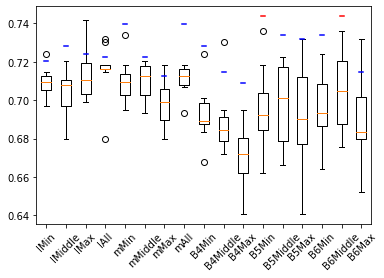
\includegraphics[scale=0.47]{results/eda/box_plot_models_acc.png}
  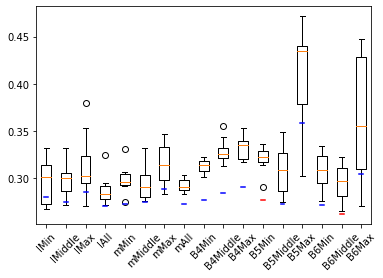
\includegraphics[scale=0.47]{results/eda/box_plot_models_mse.png}
    \caption{A box-plot of accuracy score (left) and MSE (right) of all the 17 models 
    and the blue line is ensemble-average prediction accuracy (or MSE) on the test-set. 
    The red lines are the two best ensemble-average predictions on accuracy. 
    The orange line are the mean of the 10-fold predictions.}
   \label{marker5}
  \end{minipage}
  \hfill
\end{figure}

\subsection*{Prediction by age class}

When taking the accuracy of all models by age class we found that accuracy for one- and two-year-old's was better than 90\% (figure \ref{marker6}).
All age classes six years or younger was correctly classified with more than 70\% accuracy, and all 13-year-old's was predicted to be younger (see Figure \ref{marker14} in appendix B which shows model the mean and standard deviation from the residuals test set prediction by age classes).

\begin{figure}[h!]
  \caption{Predictions by age class from the average of all models. The green region shows the correctly classified age after rounding. The axis is fixed, hence large outliers will not be visible.}
  \centering
  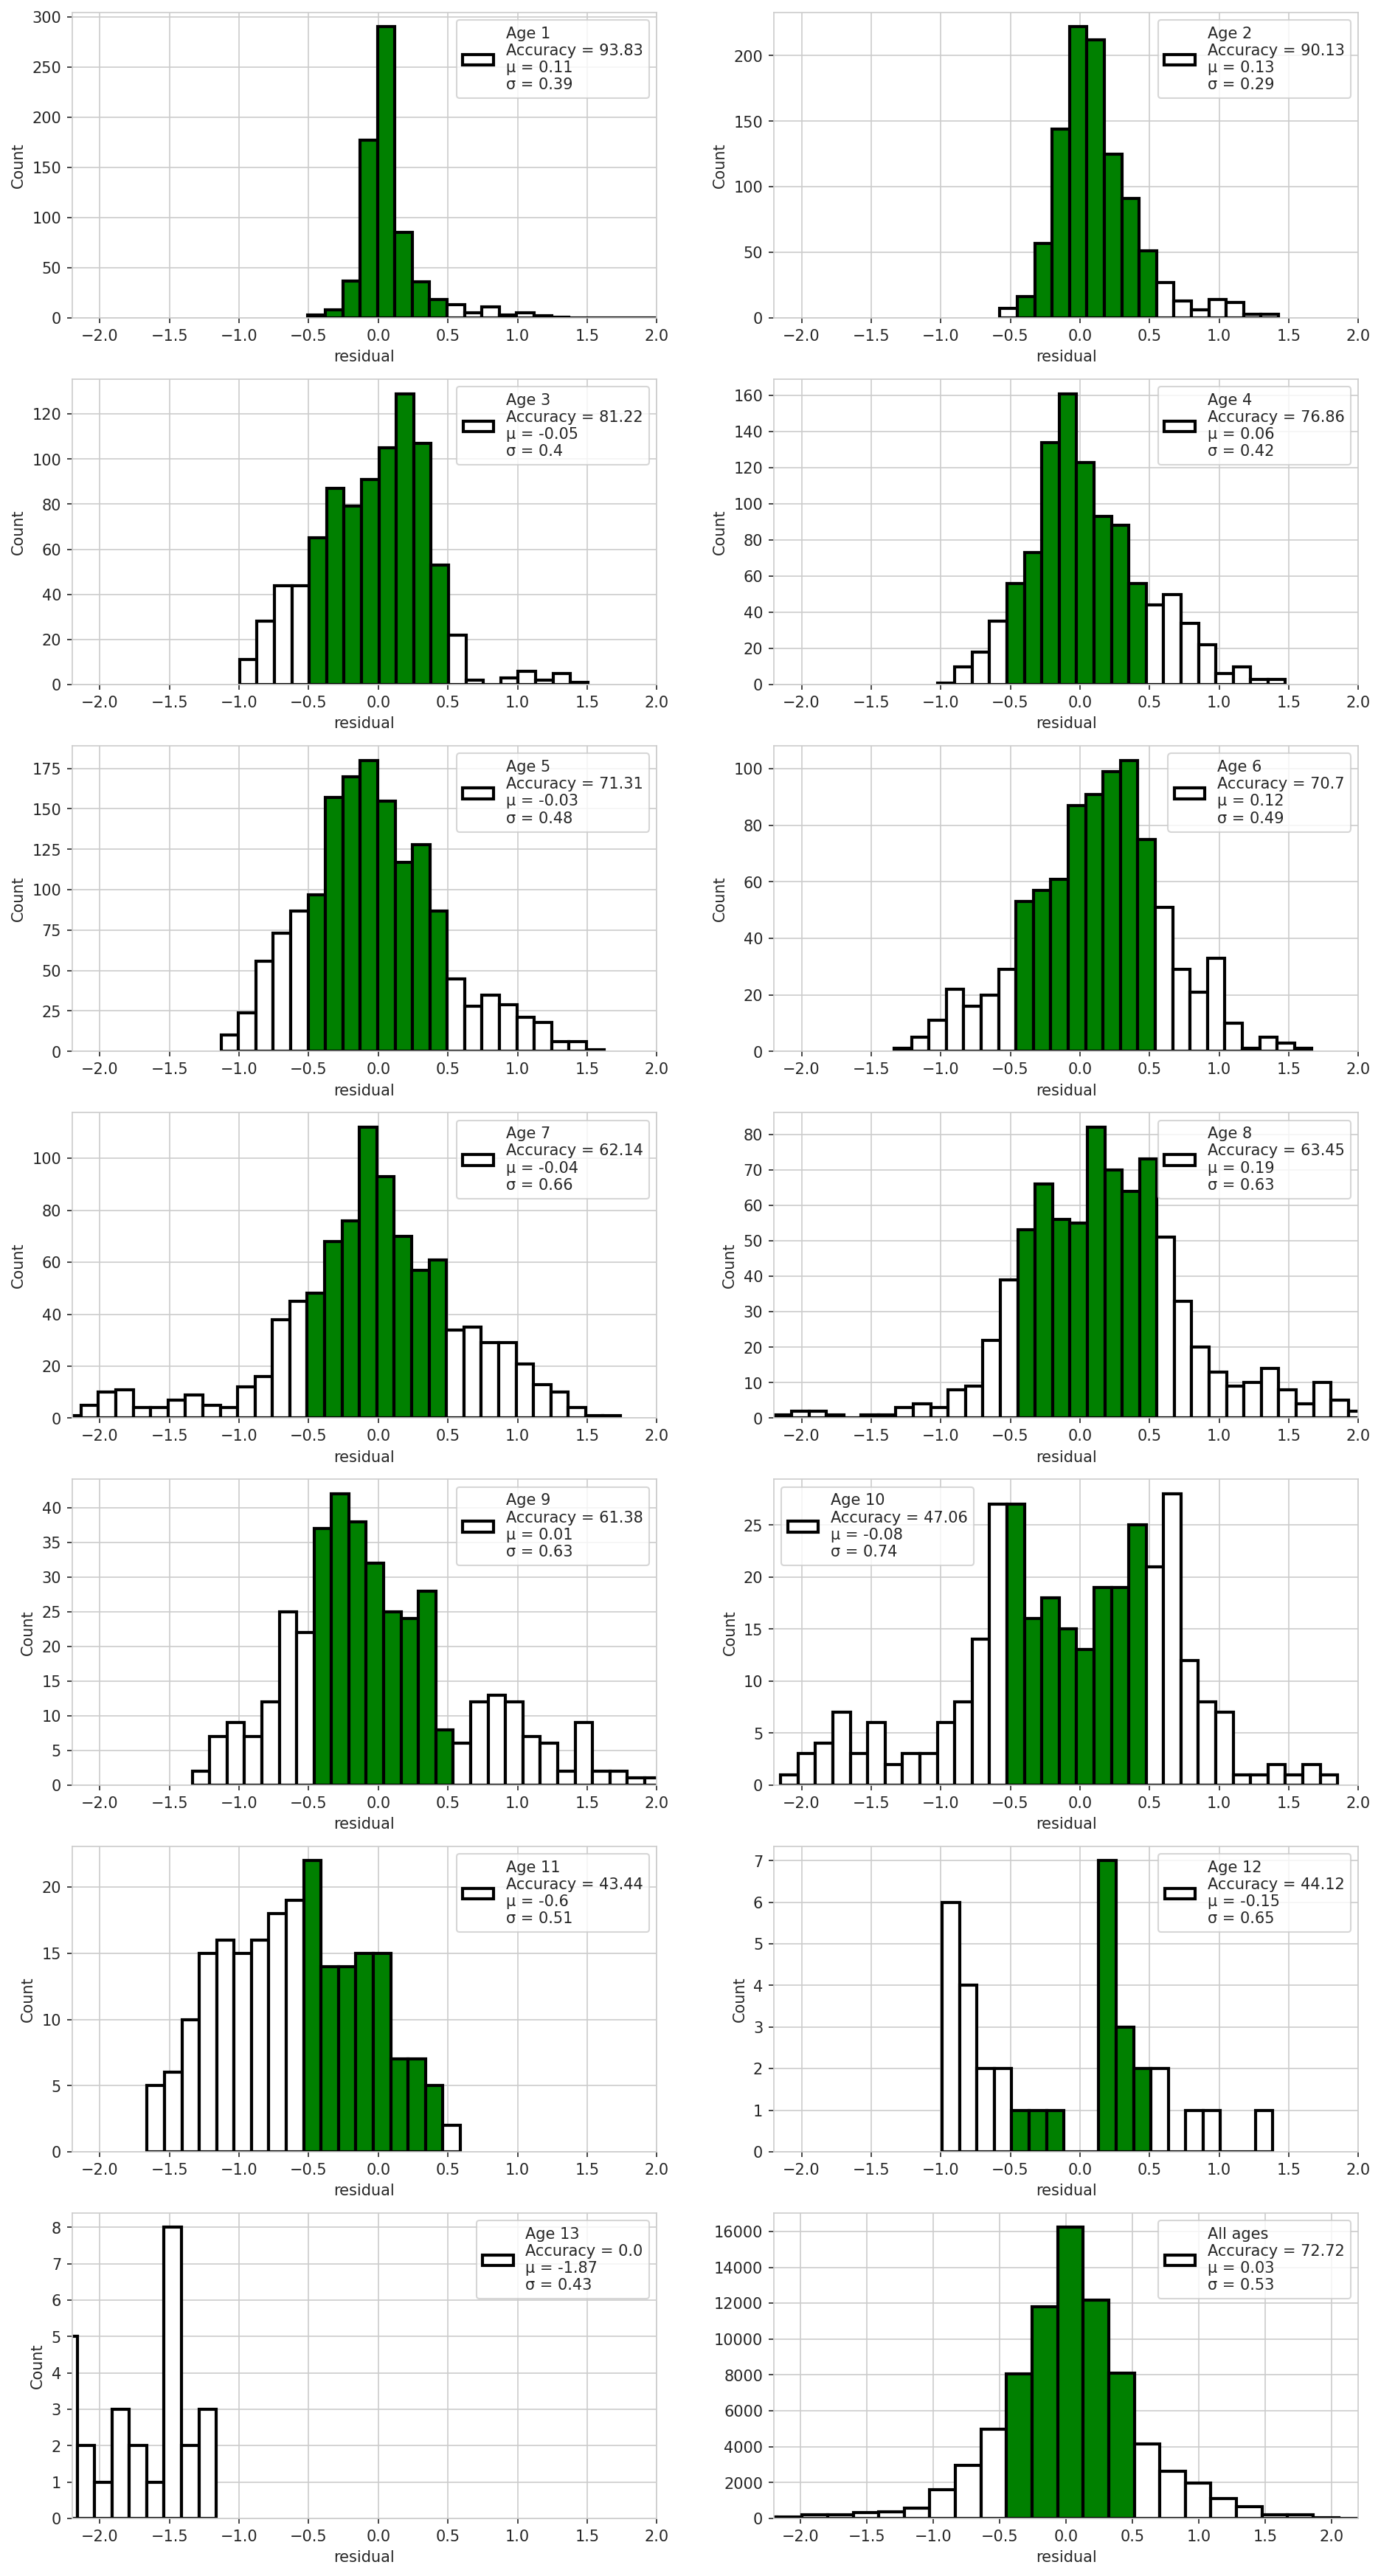
\includegraphics[scale=0.30]{results/eda/acc_by_age_dist_hist2.png}
  \label{marker6}
\end{figure}

No systematic bias in the age prediction of CNN is visible except for the underestimated age of individuals aged by human reader as 13 year old (figure \ref{marker7}).

\begin{figure}
  \centering
  \caption{Violin plot of predicted age from model B5-min with accuracy of 74.4\%. 
  Above each age is the accuracy, and below is the total number of images 
  in the test set of that age class}
  \centering
  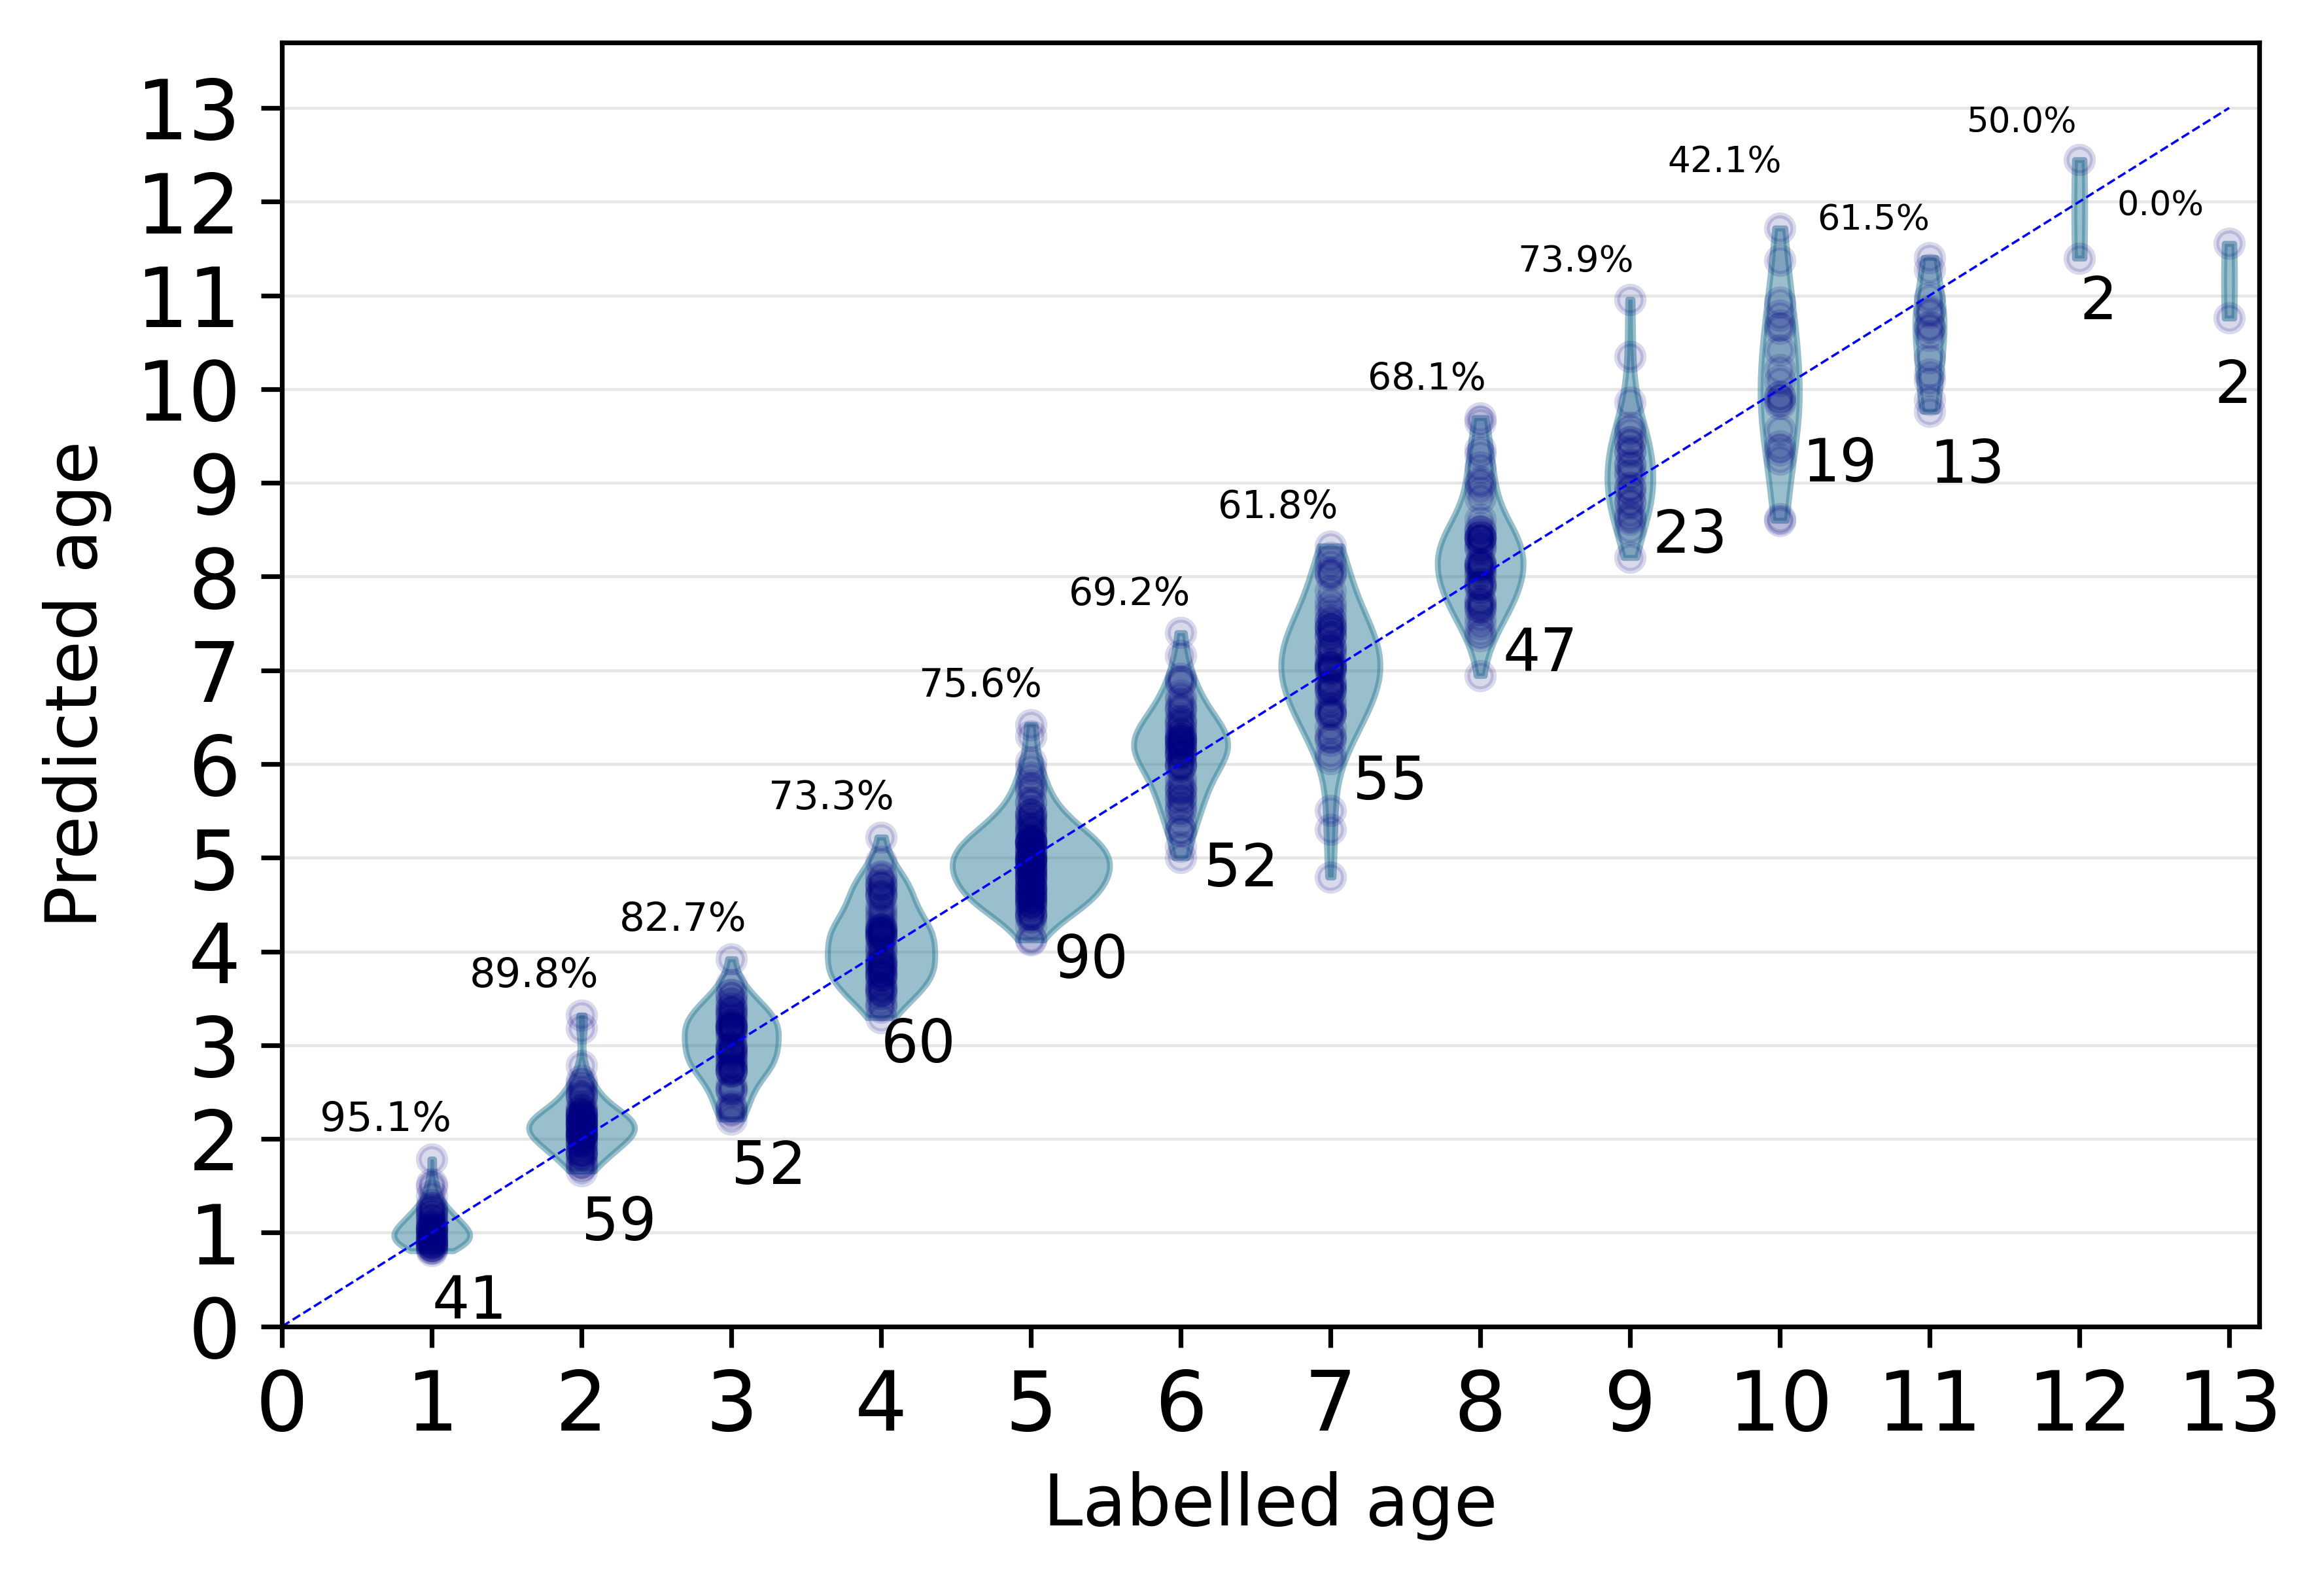
\includegraphics[scale=0.95]{results/eda/violin_plot_age.png}
  \label{marker7}
\end{figure}


\subsection*{Simple ensemble-average predictions}

We searched the space of ensembles-average predictions
of 2 to 17 models which is the set of unordered combinations without replacement,
equal to the binomial coefficient 
$\sum_{k=1}^{N}\binom{N}{k} $ where $N=17$ and $k \in 2..N$
For each set of ensemble combination we recorded the best 
ensemble and found that the best overall ensemble-average prediction 
was an ensemble of six models which produced an accuracy of 78.6\%. 
The ensemble consisted of B4-min, B5-min, B6-min, Medium-min, B6-middle, and B4-max.

Table \ref{table6} shows the number of combinations which is 
the number of ensemble models that exists with the coefficient,
the best ensemble-average accuracy on the given number of combinations,
and the model that produced the best combinations which can be
translated to model name using \ref{table1}. Table \ref{table7}
shows the a similar table but ensembles where selected to minimize MSE. 

The ensemble accuracy decreased after adding six models, while the
MSE continued to decrease until all 17 models was included.
This was as expected from the theory on simple ensemble average learning,
since the variance is reduced with more models.

\begin{center}
\begin{table}[hbt!]
\caption{Binomial combinations of simple average of ensembles accuracy}
\begin{tabular}{ |l|l|l|l| }
\hline
Coeff & \#Comb & best & model (see table \ref{table1}) \\ \hline
2 & 136 &    75.9 & (2, 5) \\ \hline
3 & 680 &    77.5 & (1, 3, 4) \\ \hline
4 & 2380 &   77.9 & (1, 2, 3, 4) \\ \hline
5 & 6188 &   77.9 & (1, 2, 3, 4, 11) \\ \hline
6 & 12376 &  78.6 & (1, 2, 3, 4, 8, 11) \\ \hline
7 & 19448 &  78.1 & (1, 2, 3, 4, 7, 8, 11) \\ \hline
8 & 24310 &  77.5 & (1, 2, 3, 4, 7, 8, 10, 11) \\ \hline
9 & 24310 &  77.5 & (1, 2, 3, 6, 7, 8, 9, 11, 17) \\ \hline
10 & 19448 & 77.1 & (1, 2, 3, 6, 7, 8, 9, 10, 12, 13) \\ \hline
11 & 12376 & 76.9 & (1, 2, 3, 4, 6, 7, 8, 10, 11, 13, 16) \\ \hline
12 & 6188 &  76.7 & (1, 3, 4, 7, 8, 10, 11, 13, 14, 15, 16, 17) \\ \hline
13 & 2380 &  76.3 & (1, 3, 4, 7, 8, 9, 10, 11, 13, 14, 15, 16, 17) \\ \hline
14 & 680 &   75.9 & (1, 2, 3, 4, 5, 8, 9, 10, 11, 12, 13, 14, 16, 17) \\ \hline
15 & 136 &   75.7 & (1, 2, 3, 4, 5, 7, 8, 9, 10, 12, 13, 14, 15, 16, 17) \\ \hline
16 & 17 &    75.5 & (1, 2, 3, 4, 5, 6, 7, 8, 9, 10, 12, 13, 14, 15, 16, 17) \\ \hline
17 & 1 &     74.8 & (1, 2, 3, 4, 5, 6, 7, 8, 9, 10, 11, 12, 13, 14, 15, 16, 17) \\ \hline
\end{tabular}
\label{table6}
\end{table}
\end{center}

\begin{center}
\begin{table}[hbt!]
\caption{Binomial combinations of simple average of ensembles MSE}
\begin{tabular}{ |l|l|l|l| }
\hline
Coeff & \#comb & best & model  (see table \ref{table1}) \\ \hline
2 & 136 & 0.319 & (12, 13) \\ \hline
3 & 680 & 0.292 & (12, 13, 15) \\ \hline
4 & 2380 & 0.279 & (12, 13, 14, 15) \\ \hline
5 & 6188 & 0.272 & (12, 13, 14, 15, 17) \\ \hline
6 & 12376 & 0.269 & (5, 10, 14, 15, 16, 17) \\ \hline
7 & 19448 & 0.268 & (5, 9, 10, 14, 15, 16, 17) \\ \hline
8 & 24310 & 0.267 & (4, 5, 9, 10, 14, 15, 16, 17) \\ \hline
9 & 24310 & 0.2643 & (4, 5, 9, 10, 12, 14, 15, 16, 17) \\ \hline
10 & 19448 & 0.262 & (4, 5, 9, 10, 12, 13, 14, 15, 16, 17) \\ \hline
11 & 12376 & 0.259 & (4, 5, 9, 10, 11, 12, 13, 14, 15, 16, 17) \\ \hline
12 & 6188 & 0.256 & (4, 5, 6, 9, 10, 11, 12, 13, 14, 15, 16, 17) \\ \hline
13 & 2380 & 0.254 & (4, 5, 6, 7, 9, 10, 11, 12, 13, 14, 15, 16, 17) \\ \hline
14 & 680 & 0.252 & (4, 5, 6, 7, 8, 9, 10, 11, 12, 13, 14, 15, 16, 17) \\ \hline
15 & 136 & 0.251 & (2, 4, 5, 6, 7, 8, 9, 10, 11, 12, 13, 14, 15, 16, 17) \\ \hline
16 & 17 & 0.250 & (1, 2, 4, 5, 6, 7, 8, 9, 10, 11, 12, 13, 14, 15, 16, 17) \\ \hline
17 & 1 & 0.248 & (1, 2, 3, 4, 5, 6, 7, 8, 9, 10, 11, 12, 13, 14, 15, 16, 17) \\ \hline
\end{tabular}
\label{table7}
\end{table}
\end{center}

We observe that model B4-min (1), and B6-min (3) was the best models with inclusion in 14 ensembles(table \ref{table8}). These models did not have the highest accuracy (74.6\%) but an accuracy of 72.8\% and 73.4\% which was lower than the the highest accuracy models which was B5-min, and B6-middle which had a rank of 3 and 5 respectively.

Exposure types by the number of times in an ensemble were ordered as follows: min-exposure (rank 4), middle-exposure (rank 9), all-exposures (rank 10), and max-exposure (rank 11.6).

\begin{center}
\begin{table}[hbt!]
\caption{Rank of number of times a model is in an ensemble}
\begin{tabular}{ |l|l|l| }
\hline
Rank & Model name & Count   \\ \hline
        1 & B4\_min & 15 \\ \hline
        1 & B6\_min & 15 \\ \hline
        3 & B5\_min & 13 \\ \hline
        3 & m\_min & 13 \\ \hline
        5 & B6\_mid & 12 \\ \hline
        6 & b5\_mid & 10 \\ \hline
        6 & B4\_max & 10 \\ \hline
        8 & l\_mid & 9 \\ \hline
        9 & B6\_max & 8 \\ \hline
        10 & m\_mid & 7 \\ \hline
%1 & B4-min & 15 \\ \hline
%1 & B6-min & 15 \\ \hline
%3 & B5-min & 13 \\ \hline
%3 & Medium-min &13 \\ \hline
%5 & B6-middle &12  \\ \hline
%6 & B5-middle &10  \\ \hline
%6 & B4-max &11 \\ \hline
%8 & Large-middle &9 \\ \hline
%9 & Large-min &8 \\ \hline
%9 & B6-max & 8 \\ \hline
%11 & Medium-middle &7 \\ \hline
%11 & Medium-all &7 \\ \hline
%11 & Large-all &7 \\ \hline
%14 & Medium-max &6 \\ \hline
%15 & B4-middle &5 \\ \hline
%15 & B5-max &5 \\ \hline
%15 & Large-max &5 \\ \hline
\end{tabular}
\label{table8}
\end{table}
\end{center}


Table \ref{table9} compares the accuracy of the best ensemble with the mean of all 17 models by age classes. The accuracy of the mean of the models was shown in figure \ref{marker5}. The table shows that the best ensemble improved the accuracy of prediction for all age classes except 13-year-old which had 0\% accuracy.
A distribution plot like figure \ref{marker5} for the best ensemble can be found in appendix D as figure \ref{marker15}.

\begin{center}
\begin{table}[hbt!]
\caption{Comparison of the mean of all the 17 models (mean) with a total accuracy of 72.7\% and 
the best ensemble model (Best Ens.) with a total accuracy of 78.6\%. In all age-groups, the
ensemble improves on the mean-model accuracy except 13 year-old.}
\setlength\tabcolsep{3.5pt} % default value: 6pt
\begin{tabular}{ |l|c|c|c|c|c|c|c|c|c|c|c|c|c|c| }
\hline
Age        & 1    & 2    & 3    & 4    & 5    & 6    & 7    &  8   & 9  & 10   & 11   & 12   & 13   \\ \hline
Mean       & 93.8 & 90.1 & 81.2 & 76.9 & 71.3 & 70.7 & 62.1 & 63.5 & 61.4 & 47.1 & 43.4 & 44.1 & 0 \\ 
Best Ens.  & 95.1 & 93.2 & 84.6 & 80.0 & 78.9 & 78.9 & 65.6 & 76.6 & 69.6 & 52.6 & 61.5 & 50.0 & 0 \\ \hline
\end{tabular}
\label{table9}
\end{table}
\end{center}

%\subsection{Draft from looking at outliers}

%13 - a lot of split rings - visible rings to be ignored, innerst section very visible, imediatly after new ring. Not normal. and it is split.  \\
%71 - very bright - all 3 axis very hard to light, plane out of focus -dorsal axis has break-line \\
%92. very good image - very old age - tight incremeants - edge zone tight \\
%270. right rings - with split zones which are in the middle zone. only missed on min, middle expo - also difficult to humen. \\
%279. good quality - split rings in mid-section \\
%308. litterly no ring - very small otolith.\\
%342. 13 year old - good quality picture. ignoring the center ring, inner section is dark ventral, distro light, dorsal side has break line \\
%362. clear and good image - and it should have been labeled as 5 year old. Registered age is wrong. \\
%369. good picture - has split rings in the middle - on bright exposures - the contrast is strong.  \\
%393. nice image - max exposure very nice image. Middle exposure not so good. Middle, and min exposure little too dark. \\ 
%There is this shadow of the otoliths outside the edge. Adds rings from background. \\
%423. Very bad image - to over-exposed. Min exposure ok-ish \\

%common outliers - split rings  - counts to much or to litle \\

\subsection*{Outliers}

Figure \ref{marker8} shows 6 images which had an error after rounding of more than 1 year. All the images with more than 1 year in prediction error are shown in table \ref{table10}, with comments by an expert on the most
common mispredictions in table \ref{table10b}. 

\begin{figure}[h!]
  \caption{Images with index 13, 71, 270, 342, 362 and 369 from the test-set
  was miss-predicted by between 25\% and 100\% of the models}
  \centering
  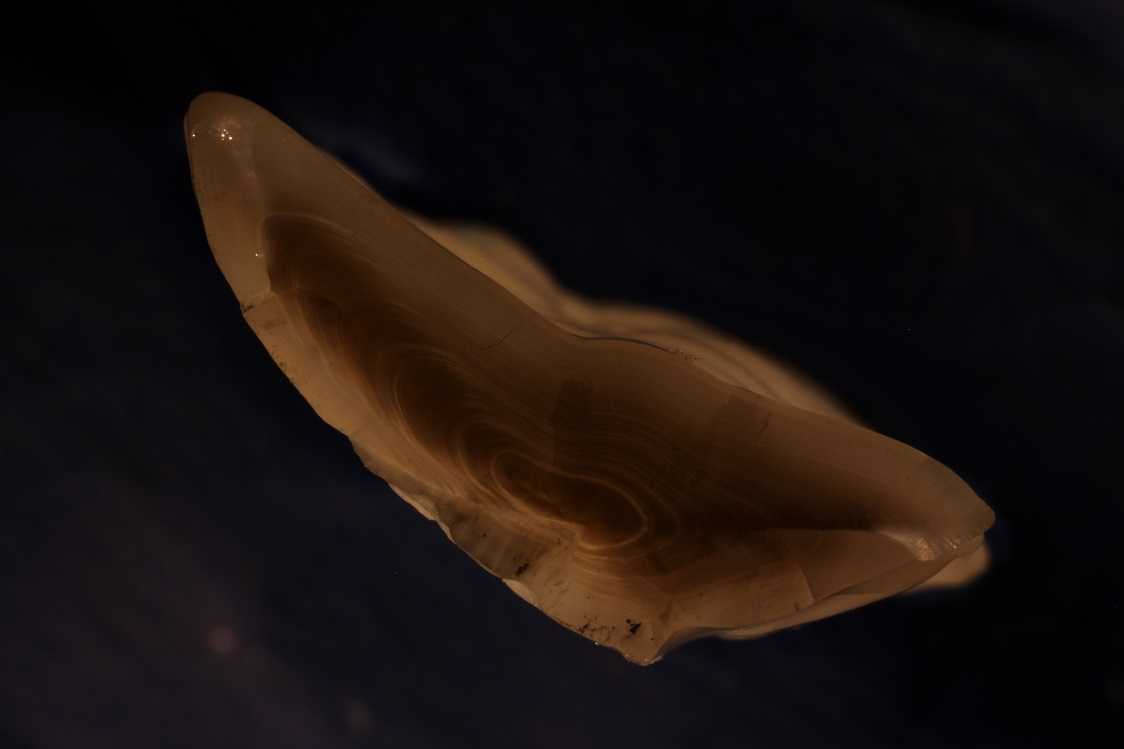
\includegraphics[scale=0.08]{outliers/IMG_0284_13.JPG}
  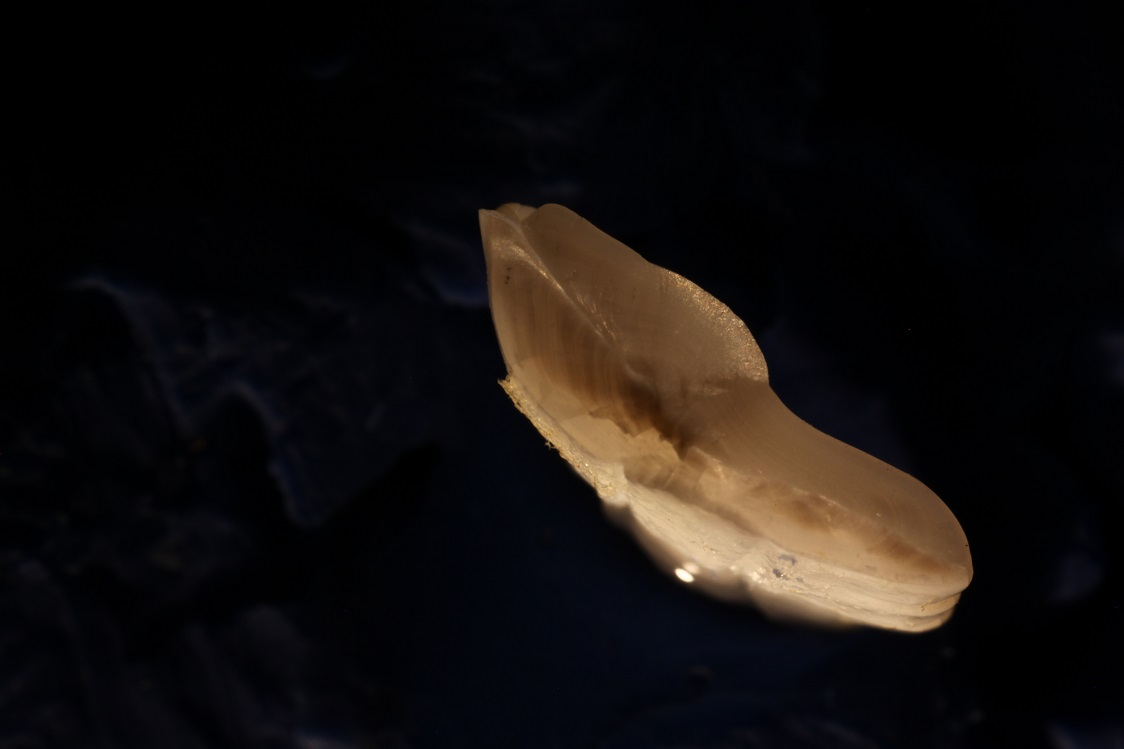
\includegraphics[scale=0.08]{outliers/IMG_0230_71.JPG}
  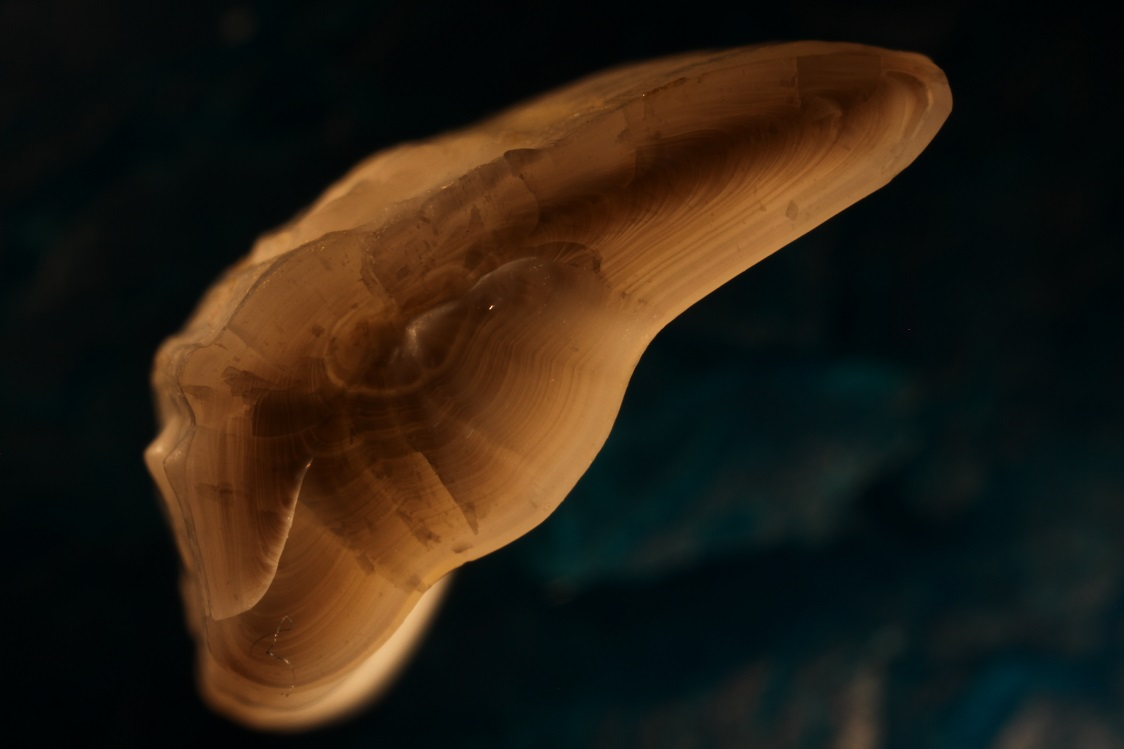
\includegraphics[scale=0.08]{outliers/IMG_0104_270.JPG} 

  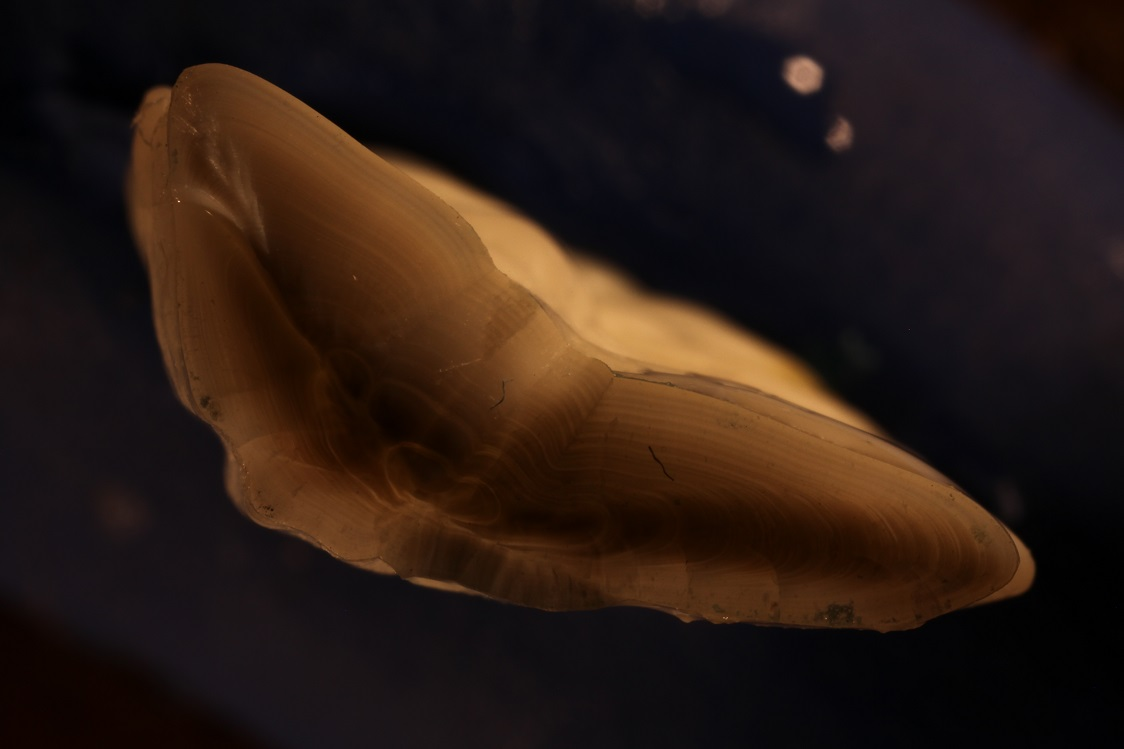
\includegraphics[scale=0.08]{outliers/IMG_0044_342.JPG}
  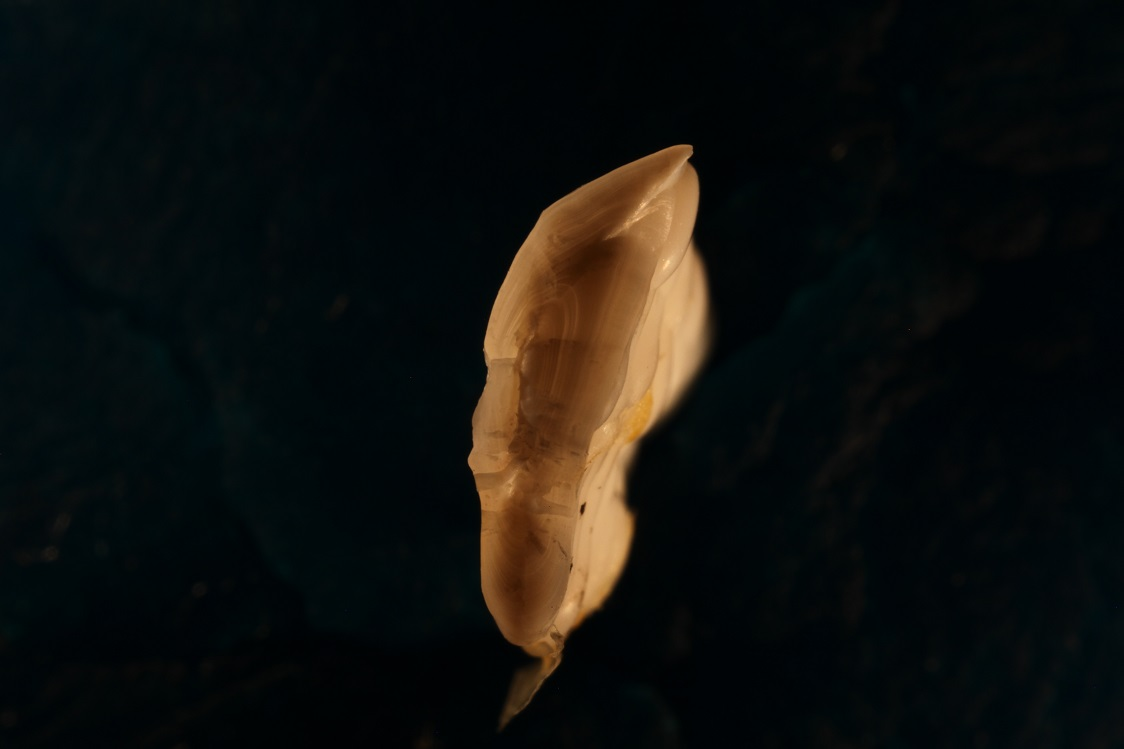
\includegraphics[scale=0.08]{outliers/IMG_0086_360.JPG}
  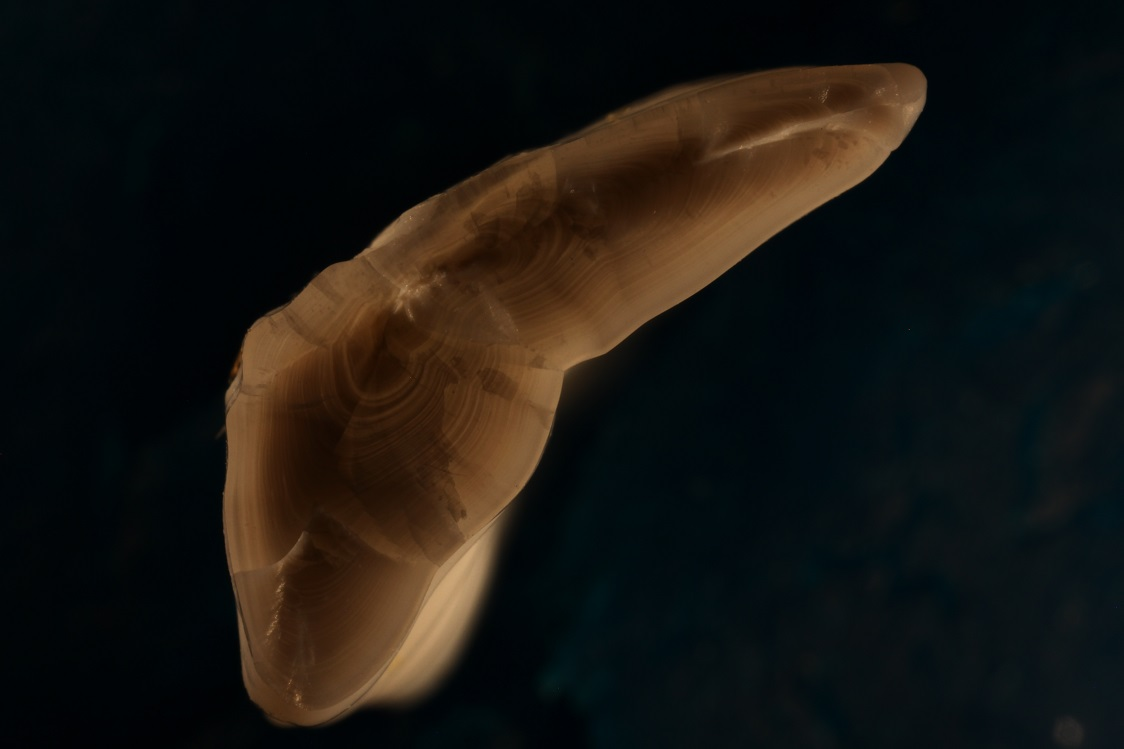
\includegraphics[scale=0.08]{outliers/IMG_0122_369.JPG}
  
  \label{marker8}
\end{figure}

We observed that there was some cod otoliths that was outliers to all models and on all exposures (e.g. otoliths 71, 342, 362, and 369),
to a family of models and on all exposures (e.g. otoliths: 13, 423), 
to some models and on one exposure (E.g otolith 308), 
and to both family of models and on some exposures (E.g. otolith 320).

We also observed that the number of large outliers did not correlate with model performance like B5-min, and B6-mid which had 7 and 9 outliers but the best  accuracy. While B4-max with the lowest accuracy (70.9\%) had the least number of large outliers with only 6 mispredictions.

\subsection*{Correlation of predictions and cluster analysis}

The correlation of models on the test-set predictions given in figure \ref{marker9} shows that the models correlates a lot on outlier predictions. The correlation from all the predictions on the test set varied between 0.988 to 0.999, with the lowest correlation found between B5-min and Medium-min. The correlation was calculated using Pearson's correlation with Euclidean distance.

\begin{figure}[h!]
  \caption{Pearson correlation of each model prediction on the test-set}
  \centering
  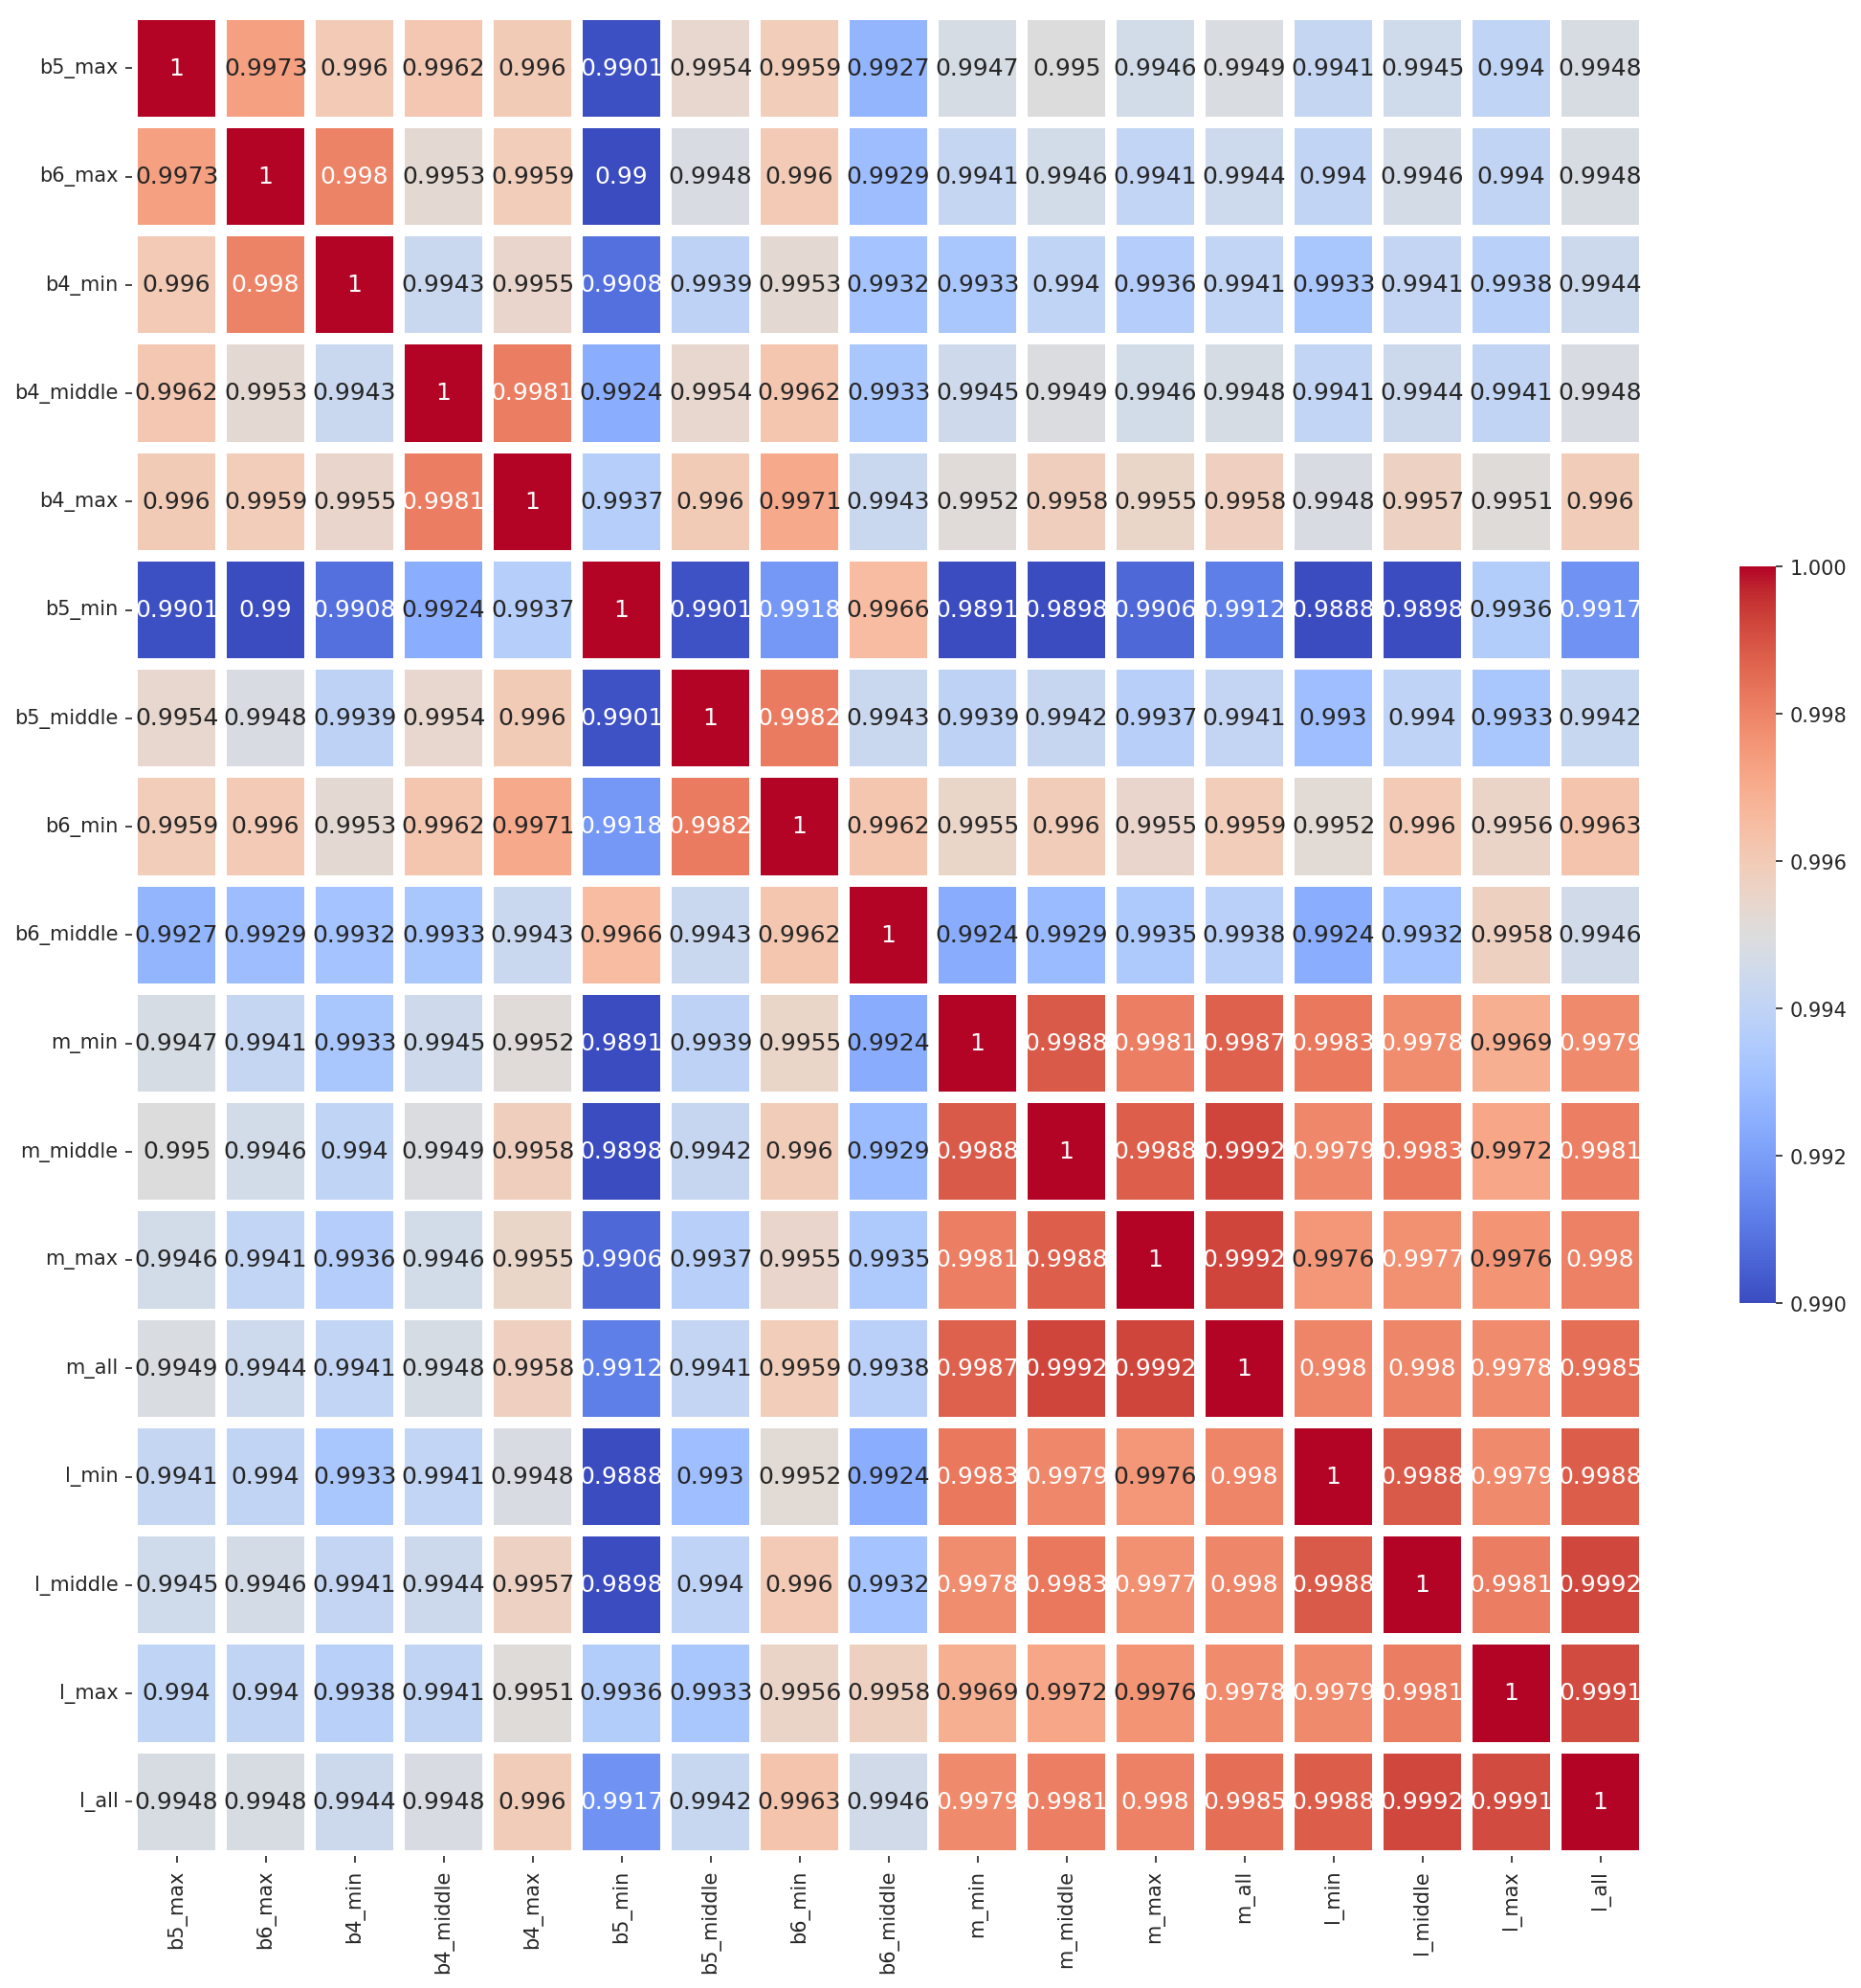
\includegraphics[scale=0.40]{results/eda/pearson_corr_models2.png}
  \label{marker9}
\end{figure}

From figure \ref{marker9} we saw that the EfficientNetV2 family was correlated from the red block in the lower right corner. The dendrogram of figure \ref{marker10} shows hierarchical clustering (HCA) of the models. HCA found 3 clusters, b5-min, and B6-middle, which are the two best models, a cluster of all the EfficientNetV2 models, and a cluster of the rest of the models (figure \ref{marker10}).

\begin{figure}[h!]
  \caption{hierarchical clustering (HCA) on correlation of predictions}
  \centering
  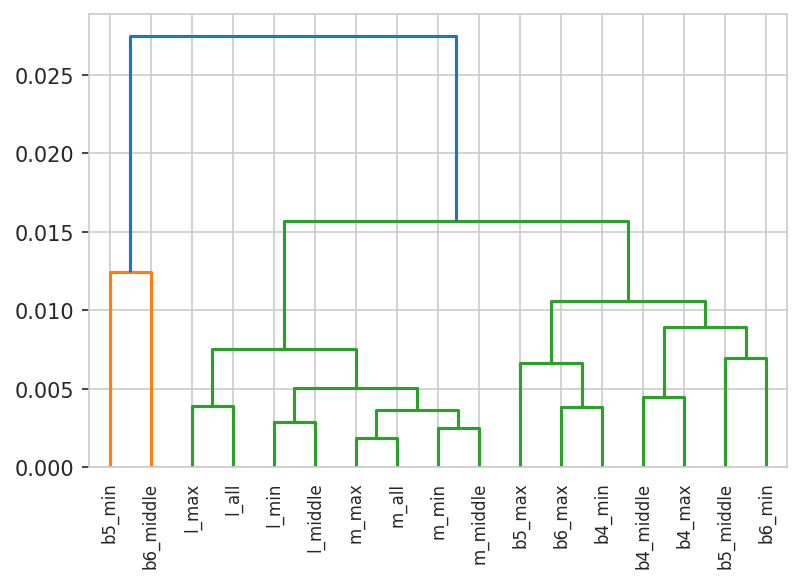
\includegraphics[scale=0.8]{results/eda/hca.png}
  \label{marker10}
\end{figure}

Using K-Means together with the elbow- and silhouette-score-methods to find the optimal number of clusters, they both found that there were 3 clusters in the correlation matrix (figure \ref{marker11}).
\begin{figure}[h!]
  \caption{1.Elbow method and 2. silhouette-score method}
  \centering
  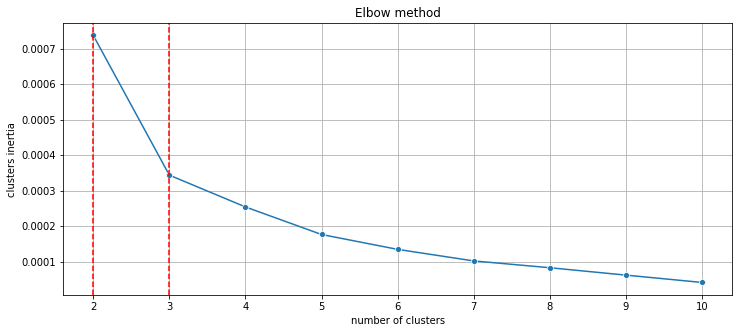
\includegraphics[scale=0.25]{results/eda/elbow.png}
  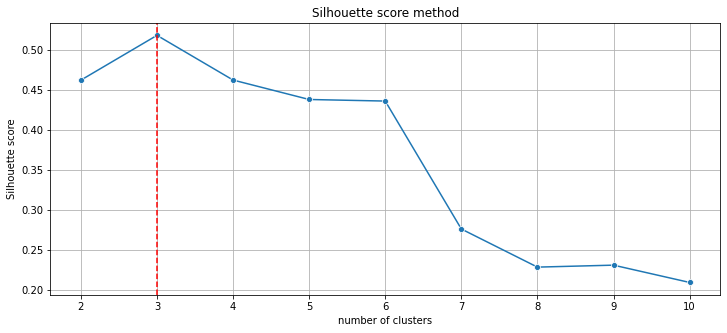
\includegraphics[scale=0.25]{results/eda/silhouette.png}
  \label{marker11}
\end{figure}

With K-Means and using 3 clusters we found similar clusters to HCA with the clusters:
\begin{itemize}
    \item B5-max, and B6-max
    \item B4-min, B5-min, B6-min, B4-middle, B5-middle, B6-middle, B4-max
    \item EfficientNetV2 family of models
\end{itemize}

Figure \ref{marker12} shows a scatter plot of two of the least correlated models, B5-min and Medium-min which had Pearson's correlation 0.988. The red point inside the two circles is not a data point but "bullseye" if both models predict the correct age. The last sub-figure was the residual correlation of all age classes. It can be viewed in more details in figure \ref{marker12b}
\begin{figure}[h!]
  \caption{Scatter plot of each age-class by Medium-min $\times$ B5-min.}
  \centering
  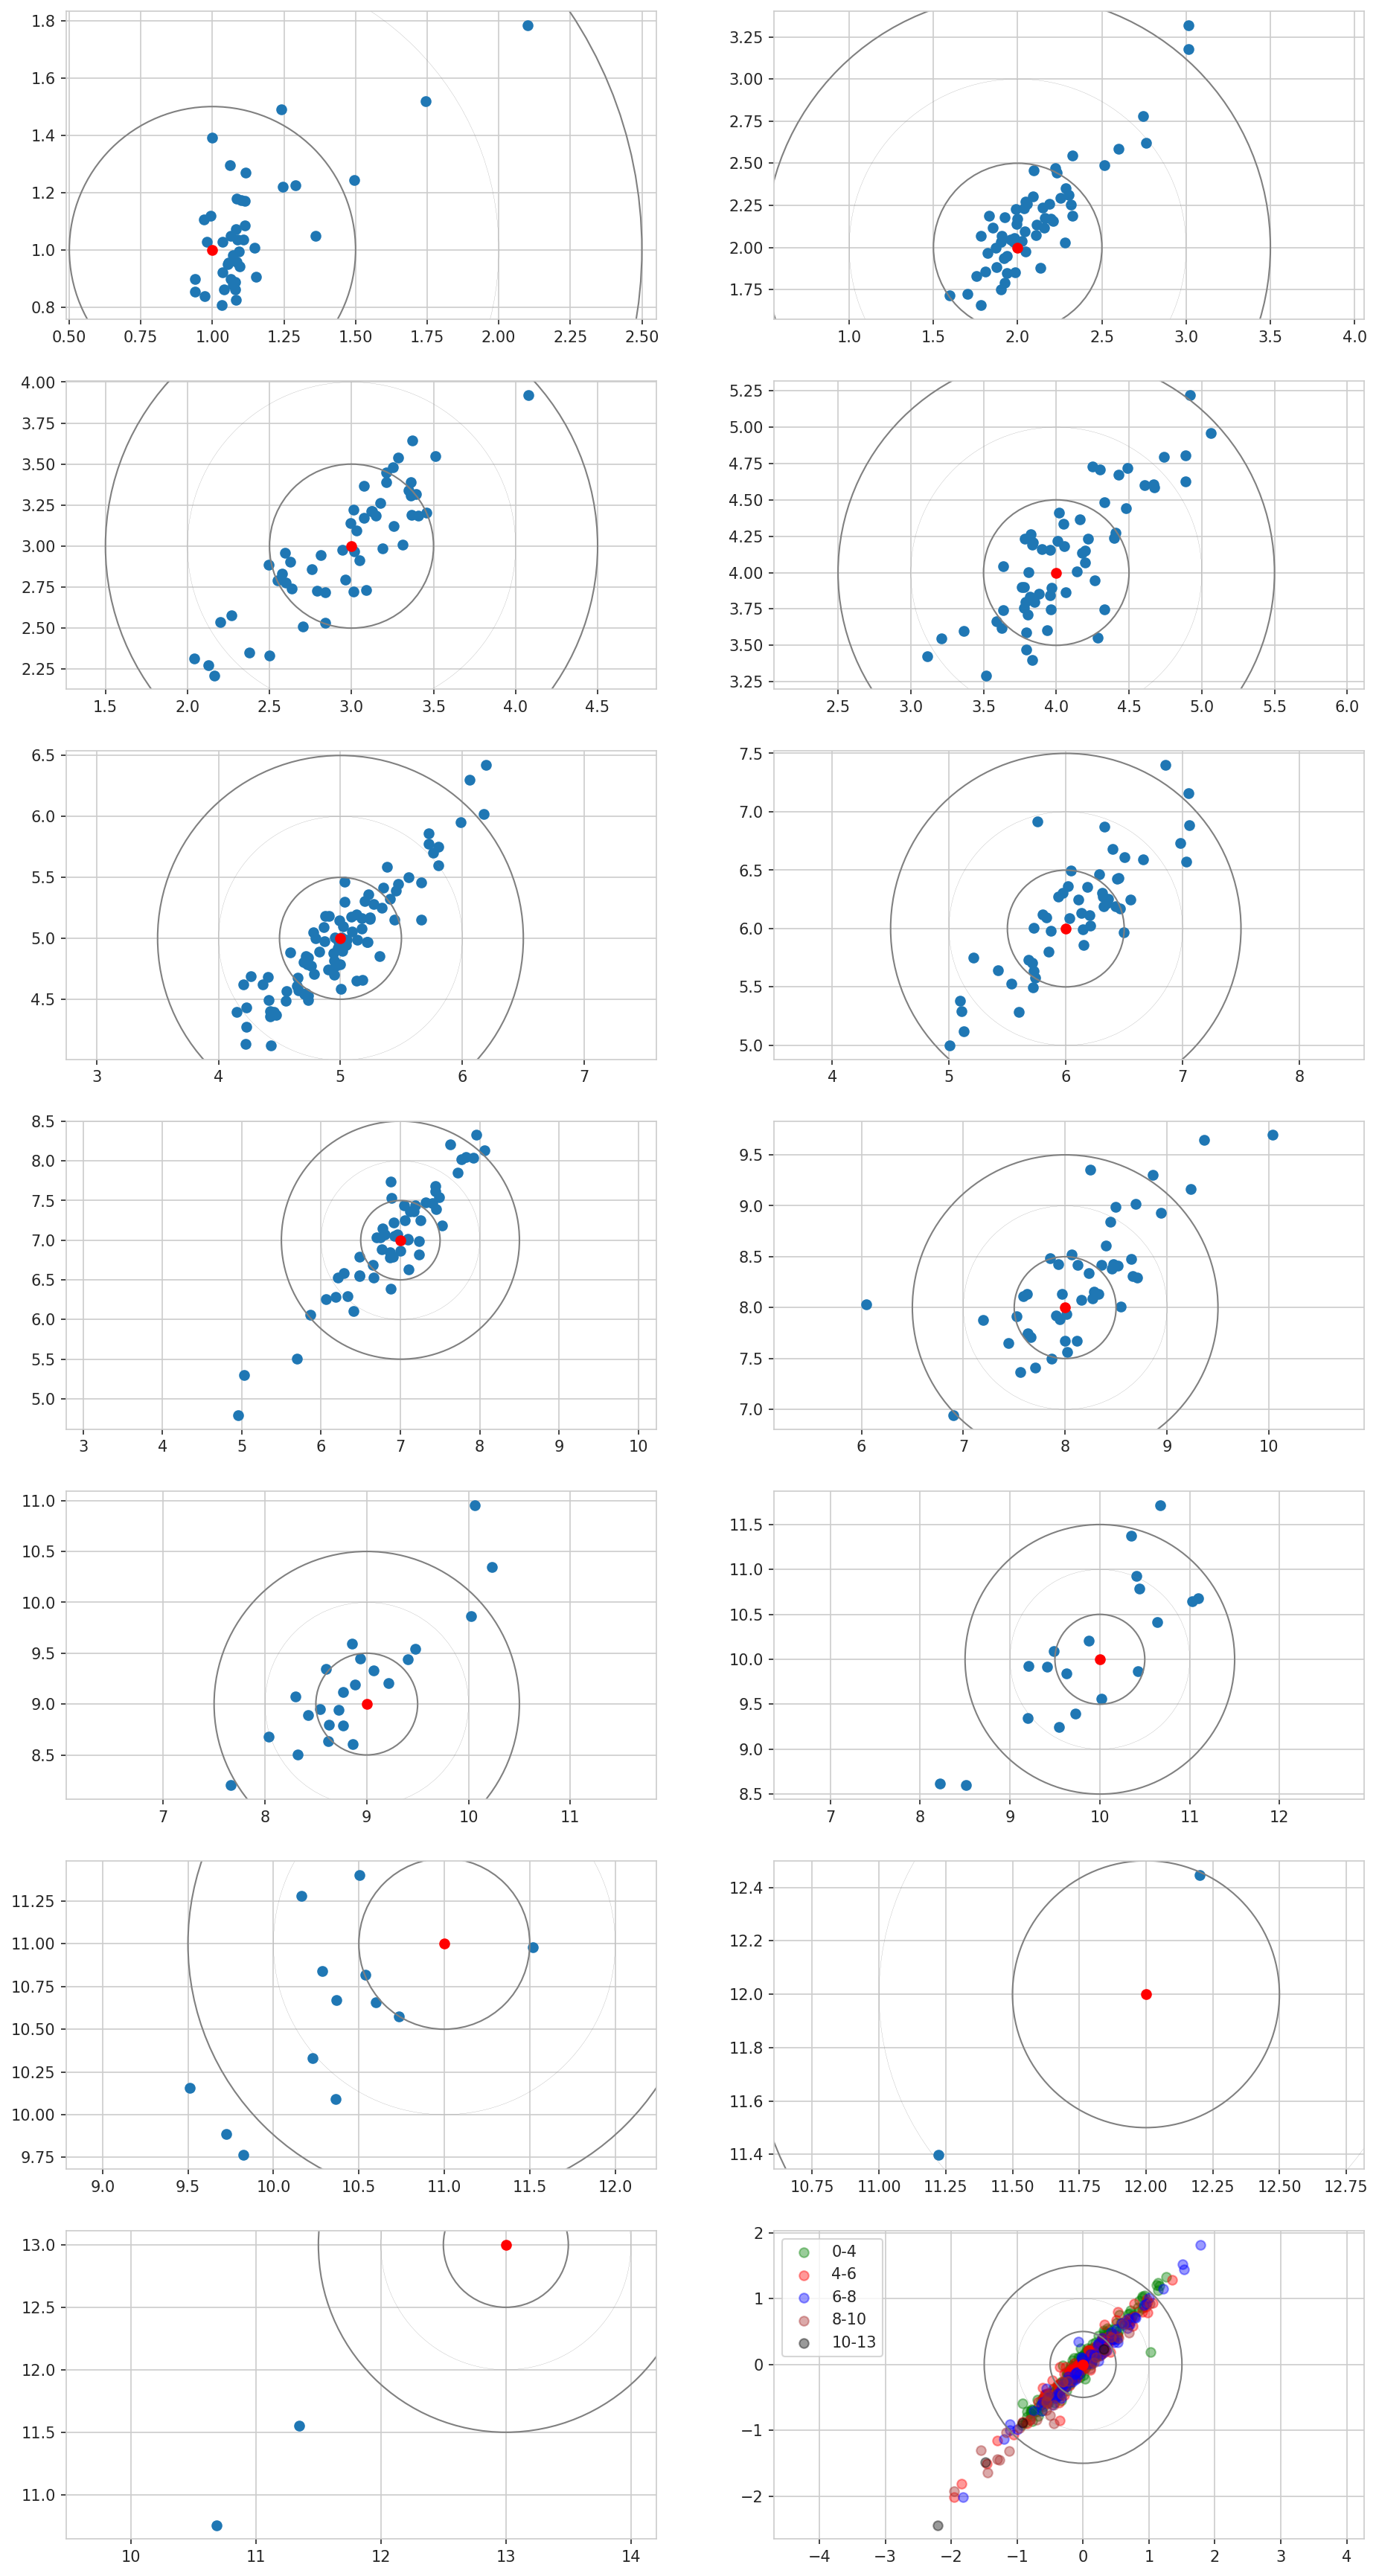
\includegraphics[scale=0.35]{results/eda/m_min_x_b5_min.png}
  \label{marker12}
\end{figure}

\begin{figure}[h!]
  \caption{Scatter plot of the residuals of all age classes by Medium-min $\times$ B5-min.}
  \centering
  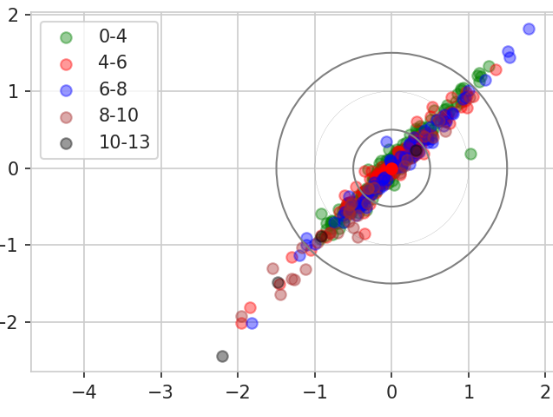
\includegraphics[scale=0.8]{results/eda/m_min_x_b5_min_residualb.png}
  \label{marker12b}
\end{figure}

\section*{Discussion}

During initial training we trained a B4 network on ca 2000 images and obtained an accuracy of ca 60\%, later another 3000 images was added and the same
network was trained on ca 5000 images which resulted in accuracy of ca 70\%.
It could be interesting to investigating if adding another 3-5000 images
would increase the accuracy to 80\%.

To reach human level accuracy a score of 85\% or higher is required ref-needed,
and a score of 90\% is considered good. Figure \ref{marker13} shows a sample of 25 predictions on the validation-set during training.

\begin{figure}[h!]
  \centering
  \begin{minipage}[b]{1.0\textwidth}
  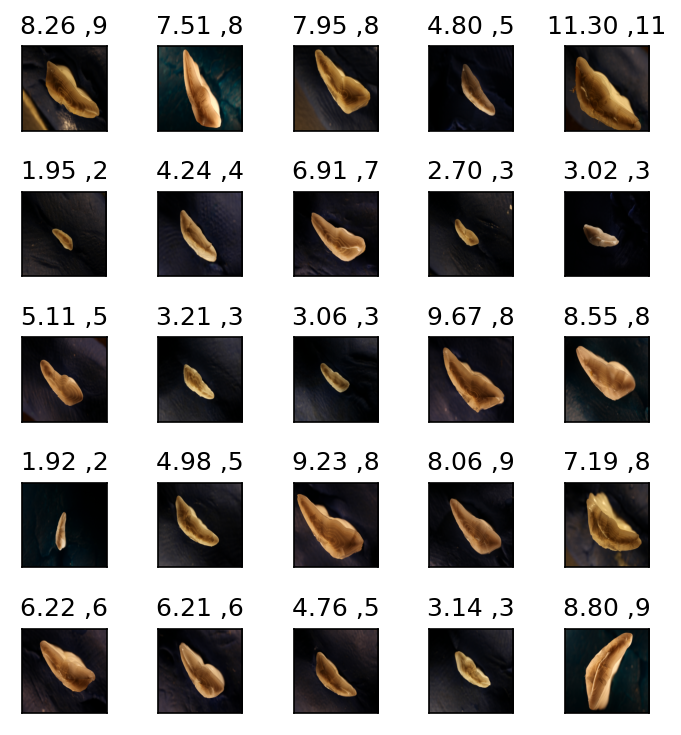
\includegraphics[scale=0.75]{results/fold_prediction_V2_m.png}
    \caption{Sample of 25 predictions on a model of training on EfficientNetV2 size medium with minimum light exposure, left number is prediction,
    and right number is age read}
   \label{marker13}
  \end{minipage}
  \hfill
\end{figure}

\subsection*{The effect of data size}

A crucial issue in machine learning projects is to determine how much training data is needed to achieve a specific performance goal. In computer vision, one commonly used rule of thumb adopted from the number of images and classes in the ImageNet dataset, is to have a thousand images for each class. In our case of cod otolith images the task entails regression towards 13 age classes instead of classification into 1000 classes. Therefore, approximately 13,000 images would appear to be the optimal number for our problem based on the rule of thumb for computer vision. This number can be reduced if transfer learning is applied for images within a similar domain. For cod otolith images, the domain is different than images in ImageNet. However, despite the different image domain for our problem we do see a significant performance boost in using transfer learning, suggesting that fewer images are needed than if trained from scratch. Excessive use of augmentation also reduces the number of images required. On the other hand, a general insight from deep learning is that more training data is always advantageous. Given the use of transfer learning and augmentation, the number of images used in this study, ~5000, might be close to the optimal but we still think that a larger training set would improve performance. During initial training we trained a B4 network on about 2000 images and obtained an accuracy of around 60%. Later  another 3000 images was added and the same network was trained on around 5000 images which resulted in accuracy of about 70%. This suggests to us that if our training set where even larger, say 10,000 images, this would boost performance further, maybe even approaching human level accuracy of 85%. 

\subsection*{Accuracy for different age classes}
All models tend to predict younger year classes with greater accuracy than older year classes. Pooling all models, prediction accuracy for 1–3 year old otoliths is > 80%, exceeding 90% for one year olds. Accuracy tends to decline with increased age, especially for otoliths older than 9 years for which the training set is less represented than for younger otoliths (Figure 2). On the other hand, age 5 is the most abundantly represented age class in the training set, and accuracy for this age class is lower than the less abundant one-year-old age class. Thus, the CNN appears to be particularly competent at analyzing cod otoliths with fewer growth zones. … Let us discuss why this is so… Ask the readers/biologists.

\subsection*{Ensemble of models}
We should discuss the improved accuracy gained when combining models into ensemble of models (table 8). The best combinations shows accuracy > 75\%.
Add a comment on the relation between variation in accuracy and the resulting accuracy of the ensemble (predictions of B4/5/6 have higher variance, but their ensembles win). 

\subsection*{Moved from introduction to Discussion –  }

Accuracy, efficiency and cost benefits of CNN classifiers versus manual reading 
…Despite fast progress the results remain mixed and often yield lower precision and consistency than those obtained by trained human readers, which limits the application of automated methods in real conditions.
However, one aspect that is often under considered by such studies are the practical time and cost benefits that implementing a functional ML framework would provide. As noted by Fisher and Hunter (2018) \citep{Fisher} in their review of digital techniques for otolith analysis, “costs for human and machine ageing systems are broadly similar since a large part of the cost is associated with preparing the otolith sections”. As such, the net benefit of automated ageing routines is directly dependent on the ability to scale performance using a comparatively smaller number of samples than human readers or, alternatively, to train them on “rougher” data that can be produced faster and at a more efficient cost.
Also, CNN can be applied without high additional cost or even be incorporated in the routine protocols, but add a new value e.g., reading consistency check, time-drifts evaluations, inter-reader comparisons (how much ‘off’ is each reader when compared to the CNN predictions, even if not compared with the same otolith samples), etc.

We see the process of CNN implementation as an evolution of the protocols, with the intensive phase of model development and training. Gradual improvement of model reliability should then allow for the application of CNN as a complementary supportive tool for the age traditional estimations. Finally, this change should aim to scale the capacity of the age reading experts and improve sampling in the areas, fish stocks, or periods that lack proper reading effort.

\subsubsection*{Conclusion}
Our results demonstrate that the use of deep learning techniques in the analysis of otoliths have a major potential for facilitating automation. We believe that carefully trained CNNs could become a major component in automated pipelines that require minimal processing and could be able to produce near at sea age estimates.

When developing the framework for the automatic age estimation it is advised to 
include B4 architectures as they are quick to train, and performs good. Ensemble approaches are also recommended if more effort is favorable, as it gives a more robust and higher performing prediction. For a quick-to-train ensemble B5, and Medium could be added. It is recommended to use under-exposed images.

\section*{References}

\bibliographystyle{apalike}
\bibliography{references}

\pagebreak

\appendix
\section{Prediction error of more than 1.5 year}

    \centering
    \captionof{table}{Predictions error with residual of more than 1.5 year per model per index in test-set}
    \rotatebox{90}{
    \setlength\tabcolsep{1.5pt} % default value: 6pt
    \renewcommand{\arraystretch}{0.8}
    \begin{tabular}{|l|l|l|l|l|l|l|l|l|l|l|l|l|l|l|l|l|l|l|l|l|l|l|l|l|}
    \hline
        Idx           & 13  & 17 & 47 & 48 & 71 & 92 & 154 & 270 & 279 & 308 & 312 & 320 & 334 & 342 & 362 & 369 & 393 & 418 & 423 &444 & 462 & 481 & 502 &  Count \\ \hline
        B4-min        & 9.8 &    &    & ~  &5.1 & ~  &     &11.7 & 9.9 & ~   & ~   & 5.5 &     &11.1 & 5.1 & 8.2 & ~   & ~   &  ~  &  ~  & ~  & ~   & ~   &  8  \\ \hline
        B4-mid        & 9.7 &    &    & ~  &5.4 & ~  &     &     &10.2 & ~   &~    & 5.4 & 7.5 &11.3 & 4.9 & 8.3 &10.6 & 9.5 &  ~  &  ~  & ~  & ~   & ~   &  10 \\ \hline
        B4-max        & 9.6 &    &    & ~  &5.0 & ~  &     &     &10.4 & ~   &~    &     &     &11.3 & 5.0 & 8.2 & ~   & ~   &  ~  &  ~  & ~  & ~   & ~   &  6  \\ \hline
        B5-min        & 9.6 &    &    & ~  &4.8 & ~  &     &11.7 & 9.7 & ~   &~    & ~   &     &10.8 & 5.3 & ~   & ~   & ~   &  ~  &11.0 & ~  & ~   & ~   &  7  \\ \hline
        B5-mid        & 9.8 &    &    & ~  &6.7 &11.5&     &11.8 & 9.8 & ~   &~    &     &     &10.9 & 5.3 & 8.4 & ~   & ~   &  ~  &10.7 & ~  & ~   & ~   &  9  \\ \hline
        B5-max        & 9.8 &    &    & ~  &4.5 &11.5&     &     & 9.6 & 7.7 &~    &     &     &10.6 & 5.1 & 8.3 & ~   & ~   &  ~  & ~   & ~  & ~   & ~   &  8* \\ \hline
        B6-min        & 9.7 &    &    &7.6 &5.1 & ~  &     & ~   & 9.7 & ~   &~    & ~   &     &10.7 & 5.2 & 7.9 &10.8 &10.7 &  ~  & ~   & ~  & ~   & 9.4 &  9  \\ \hline
        B6-mid        & 9.6 &    &    & ~  &5.1 & ~  &     &11.5 & 9.7 & ~   &~    & ~   &     &10.8 & 5.2 & 8.3 &10.8 & ~   &  ~  &     & ~  & ~   & 9.4 &  9  \\ \hline
        B6-max        & 9.8 &    &    & ~  &5.2 & ~  &     &     &     & 5.7 &~    &     &     &10.7 & 5.2 & 8.2 &10.6 & ~   &  ~  &     &6.5 & ~   & 9.4 &  9**  \\ \hline
        m-min         &     &    &    & ~  &5.0 &11.3&     &     &10.0 & ~   &~    &     &     &10.7 & 5.0 & 8.2 & ~   & ~   & 6.0 & ~   & ~  & ~   & ~   &  7  \\ \hline
        m-mid         & ~   &    &    & ~  &4.9 &11.2&     & ~   &10.0 & ~   &~    & ~   &     &10.3 & 5.1 & 8.2 & ~   &     &  ~  & ~   & ~  & ~   & ~   &  6 \\ \hline
        m-max         &     &    &6.5 & ~  &5.1 &11.2&8.7  &     &10.2 & ~   &~    &     &     &10.5 & 5.1 & 8.1 & ~   & ~   & 6.3 & ~   & ~  & ~   & ~   &  9  \\ \hline
        m-all         &     &    &    & ~  &5.0 &11.2&     &     &10.1 & ~   &~    &     &     &10.5 & 5.3 & 8.2 & ~   & ~   & 6.2 & ~   & ~  & 8.4 & ~   &  8  \\ \hline
        l-min         &     &    &    & ~  &5.1 &11.5&     &     & 9.8 & ~   &9.3  &     &     &10.7 & 5.2 & 8.3 & ~   & ~   & 5.1 & ~   & ~  & ~   & ~   &  8  \\ \hline
        l-mid         & ~   &    &    & ~  &5.0 & ~  &     & ~   & 9.8 & ~   &9.4  & 5.5 &     &10.6 & 5.2 & 8.1 &10.5 &     & 6.0 & ~   & ~  & ~   & ~   &  9  \\ \hline
        l-max         &     &9.5 &    & ~  &5.1 & ~  &     &     & 9.9 & 3.6 &~    & 5.4 &     &10.8 & 5.1 & 8.2 & ~   & ~   & 5.9 & ~   & ~  & 8.4 & ~   &  10  \\ \hline
        l-all         & ~   &9.3 &    & ~  &5.0 & ~  &     & ~   & 9.8 & ~   &     & ~   &     &10.8 & 5.2 & 8.0 &10.5 &     & 6.2 & ~   & ~  & 8.5 & ~   &  9  \\ \hline
        Age           & 8   &  8 & 8  & 6  & 7  & 13 & 7   & 10  & 8   & 1   &11   & 7   & 6   & 13  & 7   & 10  & 9   & 11  & 8  & 11   & 5   & 10 & 11  &  -  \\ \hline
        Count         & 9   &  2 & 1  & 1  &17  & 7  & 1   & 4   & 16  & 3   &2    & 2   & 1   &17   & 17  & 17  & 6   & 2   & 7  &  2   & 1   & 3  & 3   & 141 \\ \hline
        As pct        & 53  & 12 & 6  & 6  &100 & 41 & 6   & 24  & 94  & 18  &12   & 12  & 6   &100  & 100 & 100 & 35  & 12  & 41 &  12  & 6   & 18 & 18  & -  \\ \hline
    \end{tabular}
\label{table10}
}

\pagebreak
% Comments on outliers
    \centering
    \captionof{table}{Comments on the most frequently miss predicted otolith images}
    \setlength\tabcolsep{1.5pt} % default value: 6pt
    \renewcommand{\arraystretch}{0.8}
    \begin{tabular}{|l|p{13cm}|}
    \hline
        Idx & Comment \\ \hline
        13  & Labeled 8 years, and read as 10 years by the B-models (EfficentNet). \newline
              The quality of the exposures was good, but there was a lot of split rings in the middle. \\ \hline
        71  & Labeled 7 years, and read as 5 years by all models. \newline
              The exposures was very bright on all three axis, and the dorsal axis had a break line, and the plane was out of focus. \\ \hline
        279 & Labeled as 8 years, and read as 10 years by almost all models except B6-max. \newline
              The exposures was of good quality, but there was split rings in the middle. \\ \hline
        308 & Labeled as 1 year, and read as 8 years, 6 years and 4 years by B5-max, b6-max, and Large-max respectively.  \newline
              The exposures was of good quality and the predicted age is obviously wrong. \\ \hline
        342 & Labeled as 13 years, and read as 11 years by all models. The quality of the exposures was good. \newline
              The inner section is dark on the ventral side, the distro side is light, and the dorsal side has a break line.  \\ \hline
        362 & Labeled as 7 years, and read as 5 years by all models. This image is mislabeled. The otolith is obviously 5 years old.\\ \hline
        369 & Labeled as 10 years, and read as 8 years by all models except B5-min.   \newline
              The quality of the exposures was good, but it had split rings in the middle on bright exposures, and the contrast is strong. \\ \hline
        393 & Labeled as 9 years, and was read as 11 years by B4-middle, all B6 exposures and Large-middle and -all. \newline
              The middle and min exposures was too dark. Max exposure was nice. \\ \hline
        423 & Labeled as 8 years, and read as 6 years by all the EfficentNetV2 models except Medium-middle. \newline
              The quality of the images was bad. All the exposures was over-exposed. \\ \hline  
    \end{tabular}
\label{table10b}

\pagebreak

\section{Model mean and standard deviation of residual test set prediction per age class}

\begin{figure}[h!]
  \caption{Model mean and standard deviation of residual test set prediction by age class}
  \centering
  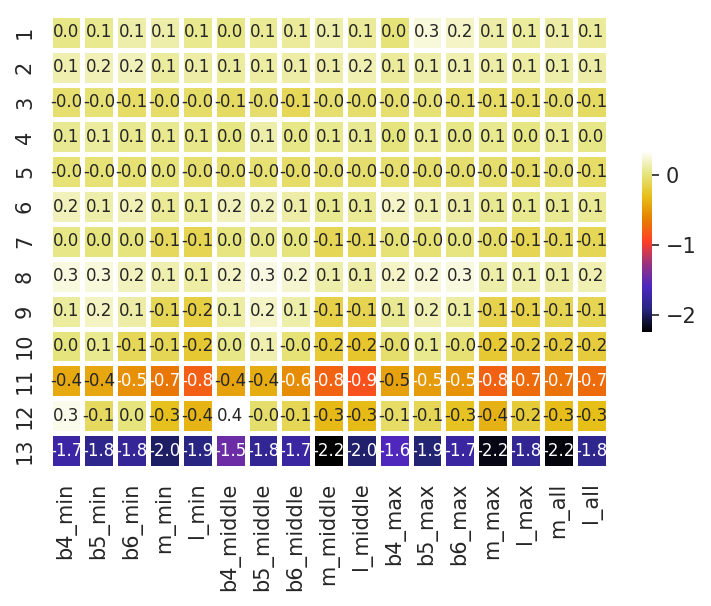
\includegraphics[width=0.82\textwidth]{results/eda/age_mean.png}
  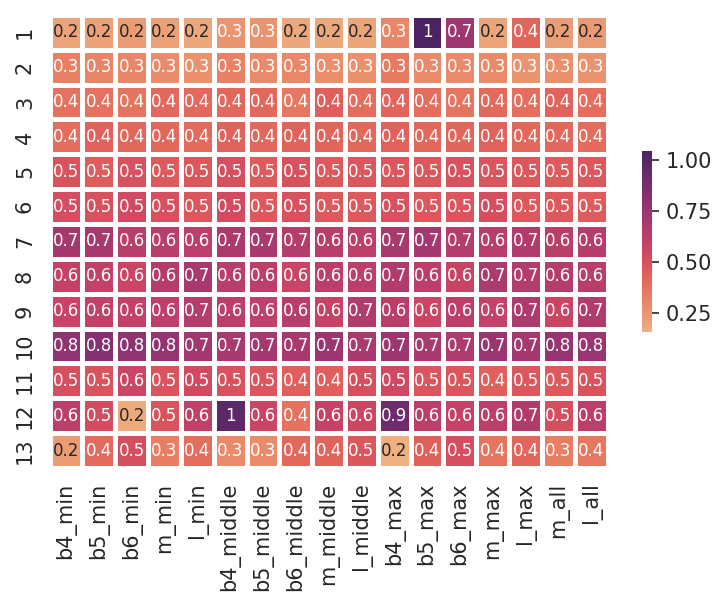
\includegraphics[width=0.82\textwidth]{results/eda/age_std.png}
  \label{marker14}
\end{figure}

\pagebreak

\section{Model accuracy and MSE per fold}

\centering
\captionof{table}{MSE per CNN per fold}
\rotatebox{90}{
    \begin{tabular}{|l|l|l|l|l|l|l|l|l|l|l|l|l|}
    \hline
        CNN/fold  & 1    & 2    & 3    & 4    & 5    & 6    & 7    & 8    & 9    & 10   & ens. & Mean \\ \hline
        B4,min    & .320 & .318 & .306 & .313 & .322 & .314 & .315 & .316 & .306 & .302 & .277 & .313 \\ \hline
        B4,middle & .344 & .328 & .316 & .334 & .326 & .320 & .355 & .326 & .313 & .325 & .285 & .329 \\ \hline
        B4,max    & .340 & .317 & .318 & .347 & .336 & .336 & .336 & .320 & .354 & .336 & .291 & .334 \\ \hline
        B5,min    & .324 & .322 & .325 & .336 & .291 & .314 & .320 & .331 & .33  & .317 & .277 & .321 \\ \hline
        B5,middle & .308 & .286 & .315 & .349 & .332 & .310 & .280 & .275 & .331 & .288 & .273 & .307 \\ \hline
        B5,max    & .472 & .302 & .437 & .459 & .432 & .366 & .356 & .441 & .438 & .418 & .359 & .412 \\ \hline
        B6,min    & .325 & .329 & .334 & .293 & .312 & .290 & .320 & .300 & .276 & .306 & .272 & .309 \\ \hline
        B6,middle & .323 & .301 & .312 & .268 & .294 & .266 & .309 & .311 & .278 & .289 & .262 & .295 \\ \hline
        B6,max    & .435 & .306 & .306 & .270 & .390 & .321 & .411 & .321 & .294 & .448 & .305 & .350 \\ \hline
        m,min     & .292 & .292 & .294 & .275 & .298 & .304 & .304 & .331 & .307 & .295 & .273 & .299 \\ \hline
        m,middle  & .287 & .302 & .307 & .332 & .288 & .276 & .277 & .294 & .304 & .278 & .278 & .295 \\ \hline
        m,max     & .337 & .297 & .302 & .291 & .315 & .347 & .338 & .321 & .313 & .283 & .289 & .314 \\ \hline
        m,all     & .289 & .299 & .303 & .284 & .292 & .287 & .303 & .288 & .289 & .294 & .273 & .293 \\ \hline
        l,min     & .267 & .316 & .269 & .270 & .322 & .332 & .280 & .307 & .303 & .299 & .280 & .297 \\ \hline
        l,middle  & .300 & .332 & .320 & .300 & .272 & .302 & .294 & .285 & .307 & .285 & .275 & .300 \\ \hline
        l,max     & .322 & .295 & .324 & .353 & .295 & .306 & .271 & .292 & .380 & .299 & .286 & .314 \\ \hline
        l,all     & .285 & .293 & .283 & .274 & .286 & .325 & .272 & .283 & .277 & .295 & .271 & .287 \\ \hline
        Mean      & .328 & .308	& .316 & .315 &	.318 & .313 & .314 & .314 & .318 & .315	& .284 & .316 \\ \hline
    \end{tabular}
    \label{table11}    
}

\pagebreak
\centering
\captionof{table}{Accuracy per CNN per fold}
\rotatebox{90}{
    \begin{tabular}{|l|l|l|l|l|l|l|l|l|l|l|l|l|}
    \hline
        CNN/fold   & 1    & 2    & 3    & 4    & 5    & 6    & 7    & 8    & 9    & 10   & ens. & Mean \\ \hline
        B4, min    & 69.9 & 68.9 & 68.7 & 68.3 & 68.9 & 70.1 & 69.7 & 66.8 & 68.9 & 72.4 & 72.8 & 69.3 \\ \hline
        B4, middle & 68.5 & 69.3 & 73.0 & 68.5 & 67.8 & 68.2 & 67.2 & 67.2 & 68.3 & 69.5 & 71.5 & 68.8 \\ \hline
        B4, max    & 64.1 & 68.2 & 67.2 & 66.2 & 67.8 & 69.5 & 67.2 & 69.3 & 66.2 & 65.2 & 70.9 & 67.1 \\ \hline
        B5, min    & 71.8 & 69.1 & 69.3 & 66.8 & 73.6 & 70.7 & 66.2 & 68.3 & 69.5 & 68.7 & 74.4 & 69.4 \\ \hline
        B5, middle & 70.3 & 72.0 & 67.8 & 66.6 & 67.4 & 69.9 & 71.8 & 71.5 & 68.2 & 72.2 & 73.4 & 69.8 \\ \hline
        B5, max    & 71.3 & 71.1 & 67.4 & 73.2 & 66.4 & 68.9 & 64.1 & 69.1 & 68.7 & 71.8 & 73.2 & 69.2 \\ \hline
        B6, min    & 68.3 & 68.5 & 66.4 & 72.4 & 70.7 & 70.9 & 69.3 & 69.3 & 72.0 & 68.9 & 73.4 & 69.7 \\ \hline
        B6, middle & 68.5 & 69.9 & 67.6 & 73.6 & 72.8 & 72.0 & 68.0 & 69.3 & 72.0 & 71.1 & 74.4 & 70.5 \\ \hline
        B6, max    & 70.5 & 68.2 & 65.2 & 73.2 & 69.1 & 67.8 & 68.0 & 68.0 & 72.8 & 68.5 & 71.5 & 69.1 \\ \hline
        m, min     & 71.1 & 71.1 & 69.5 & 73.4 & 71.8 & 70.9 & 70.9 & 69.7 & 70.1 & 71.5 & 74.0 & 71.0 \\ \hline
        m, middle  & 71.3 & 70.1 & 70.1 & 70.9 & 71.7 & 71.8 & 72.0 & 71.3 & 69.3 & 71.8 & 72.4 & 71.0 \\ \hline
        m, max     & 68.9 & 70.1 & 70.3 & 71.3 & 70.7 & 68.5 & 69.7 & 68.0 & 69.1 & 71.8 & 71.3 & 69.8 \\ \hline
        m, all     & 71.7 & 70.7 & 69.3 & 71.3 & 71.8 & 71.8 & 71.3 & 71.7 & 71.1 & 70.7 & 74.0 & 71.1 \\ \hline
        l, min     & 72.4 & 69.7 & 71.5 & 70.8 & 71.3 & 71.3 & 70.9 & 69.9 & 71.1 & 70.5 & 72.0 & 71.0 \\ \hline
        l, middle  & 68.7 & 68.0 & 69.7 & 71.8 & 71.1 & 71.1 & 69.7 & 70.5 & 71.1 & 72.0 & 72.8 & 70.4 \\ \hline
        l, max     & 71.1 & 70.1 & 69.9 & 74.2 & 72.8 & 71.1 & 72.2 & 71.1 & 71.1 & 70.1 & 72.4 & 71.4 \\ \hline
        l, all     & 71.8 & 71.7 & 71.8 & 71.7 & 71.7 & 68.0 & 73.2 & 71.7 & 73.0 & 71.5 & 72.2 & 71.6 \\ \hline
        Mean       & 70.0 & 69.8 & 69.1 & 70.8 & 70.4 & 70.1 & 69.5 & 69.6 & 70.1 & 70.5 & 72.7 & 70.0 \\ \hline
    \end{tabular}
\label{table12}    
}

\pagebreak
\section{Prediction per age class  using from best ensemble}
\centering
\begin{figure}[h!]
  \caption{Predictions by age class from the best ensemble.}
  \centering
  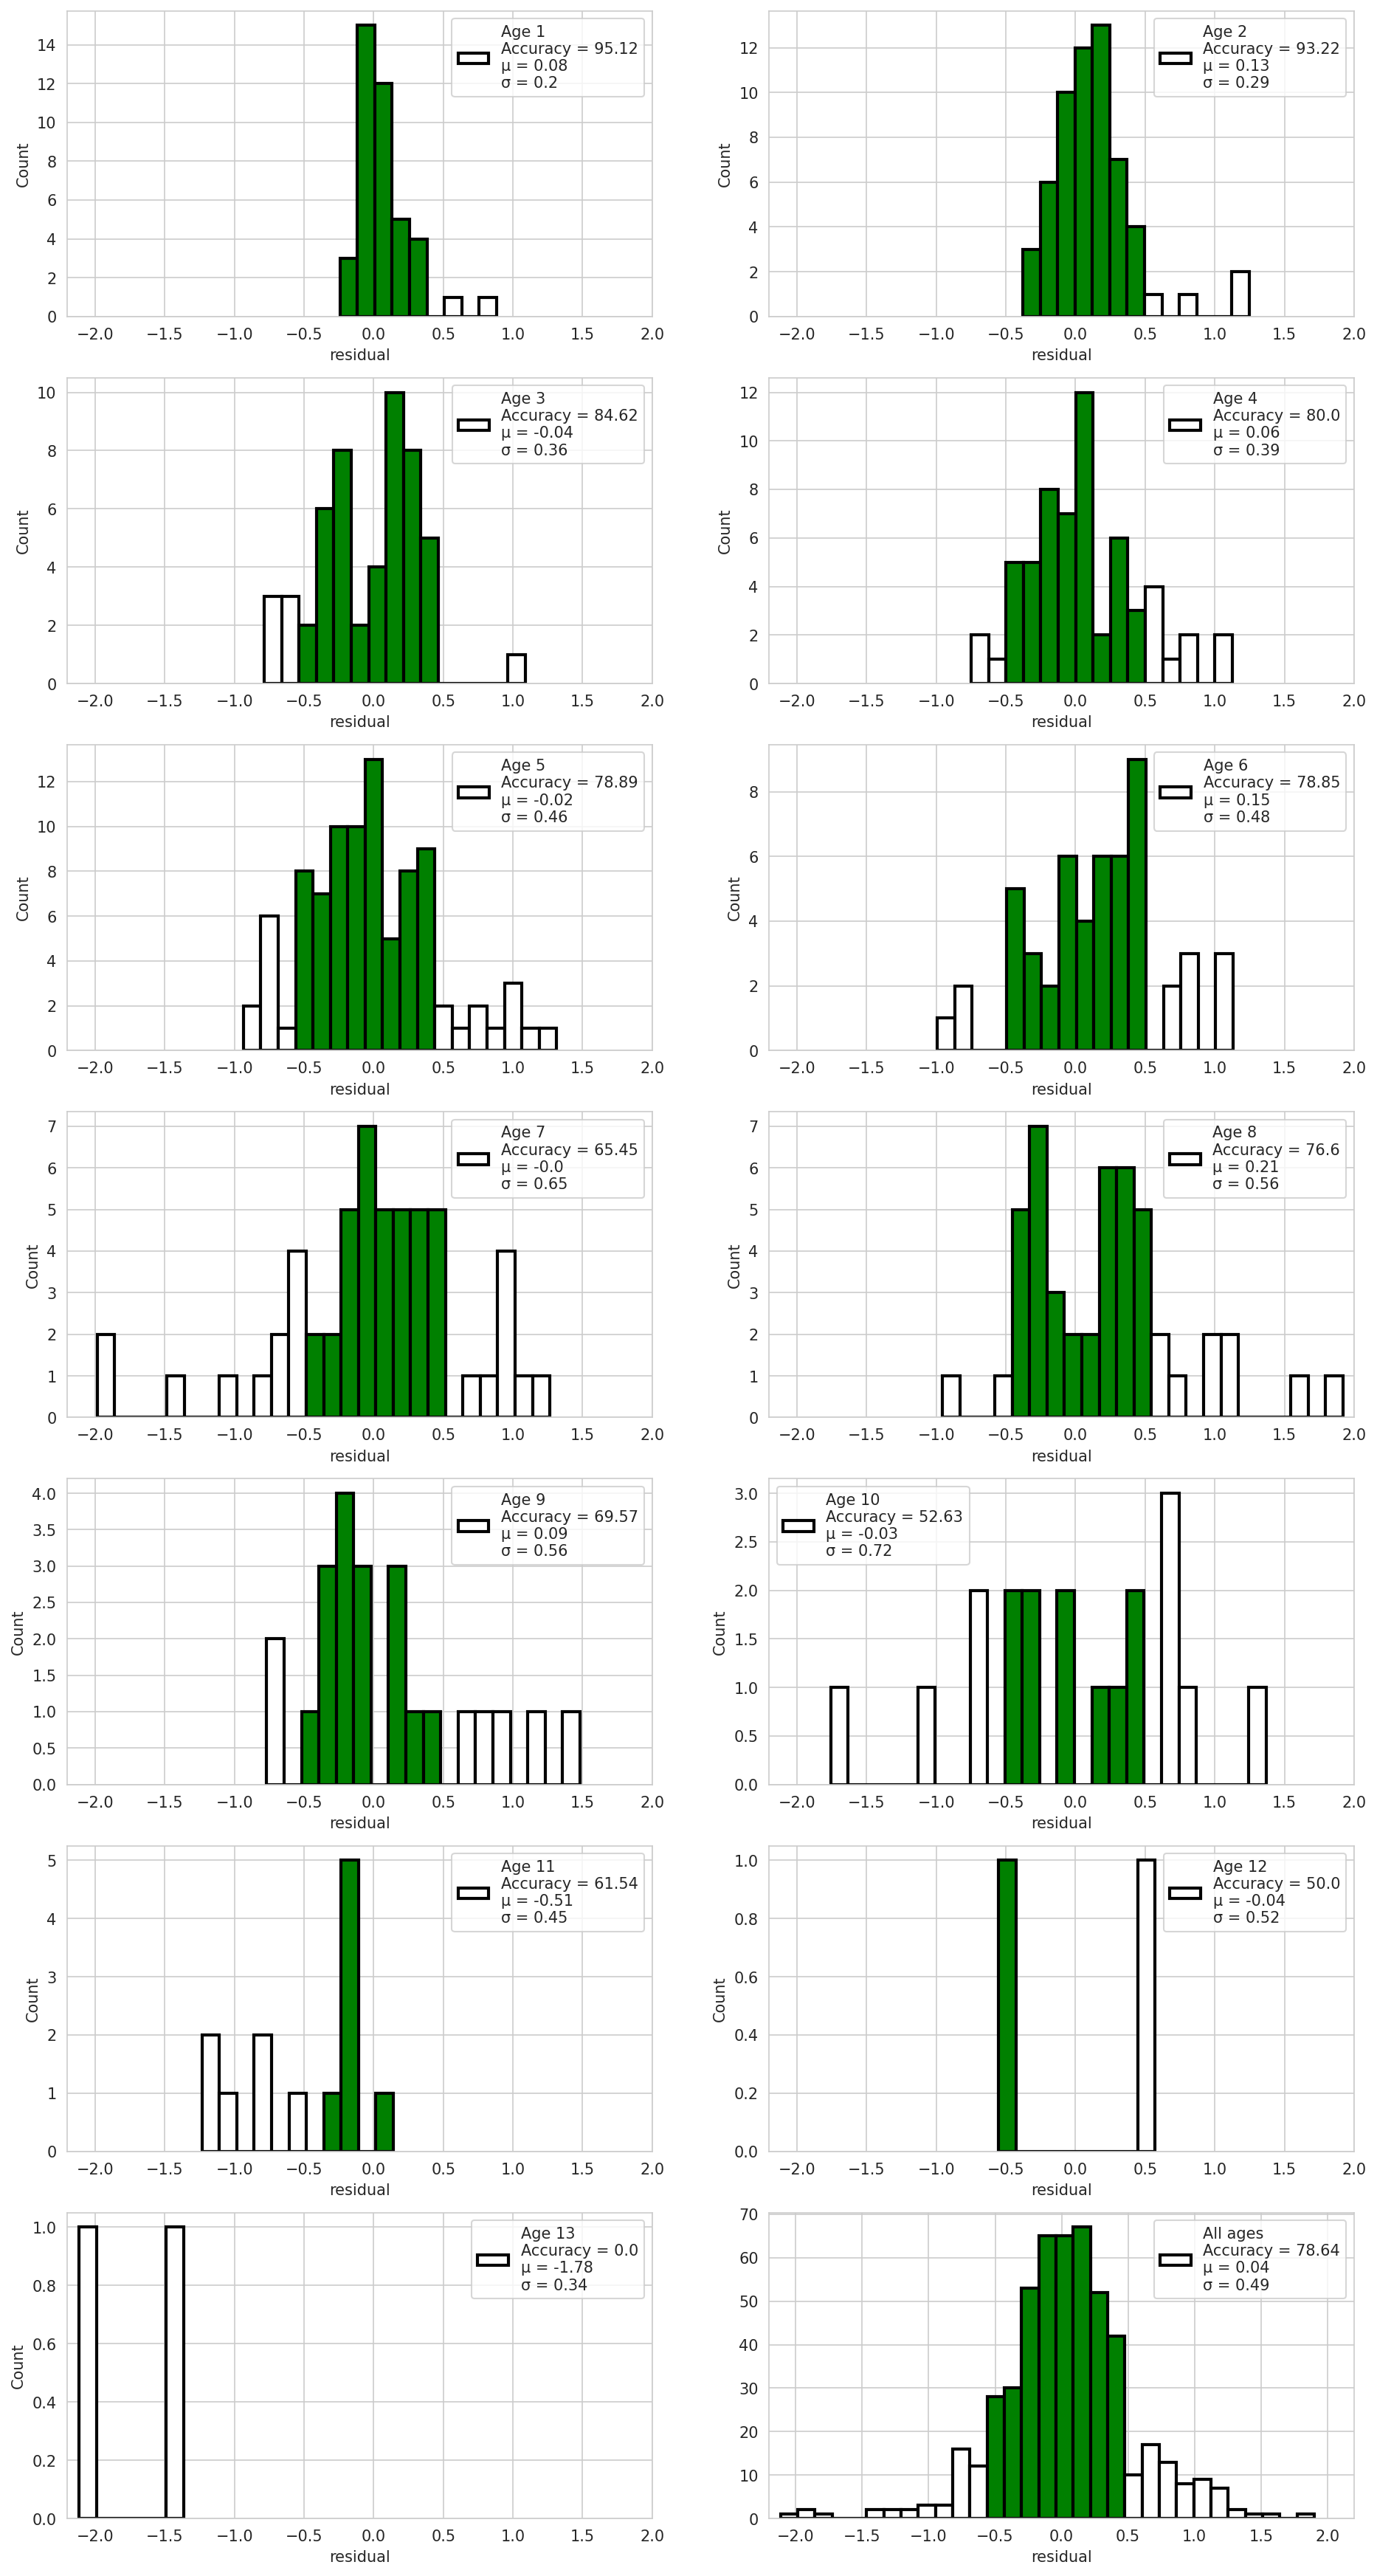
\includegraphics[scale=0.34]{results/eda/acc_by_age_dist_best_ensemble_hist2.png}
  \label{marker15}
\end{figure}

\end{document}
